\documentclass[11pt, a5paper]{memoir}

% I think I need to go back through and better clarify what the difference is between operators in the npcfs and numbers in the path integral. How do anti particles and incoming vs outgoing particles manifest themselves in both?
% paperwidth=6in, paperheight=9in, 
\usepackage[top=0.9in, bottom=1in, left=0.8in, right=0.8in]{geometry}
\usepackage[compat=1.1.0]{tikz-feynman}
\usepackage{imakeidx} % Index
\usepackage{amsmath}
\usepackage{amssymb}
\usepackage{tikz}
\usepackage{environ}
\usepackage{bm}
\usepackage{braket}
\usepackage{setspace}
\usepackage{makecell}
\usepackage{dsfont}
\usepackage{fancyhdr}
\usepackage{etoolbox}
\usepackage{ifthen}
\usepackage{siunitx}
\usepackage{slashed}
\usepackage[explicit,compact]{titlesec} % For changing the chapter layout
\usepackage[T1]{fontenc}
\usepackage{crimson}
\usepackage[hidelinks]{hyperref}

\newcounter{mycounter}
\NewEnviron{e}[1][]{\begin{equation}\BODY\end{equation}}
\NewEnviron{es}[1][]{\begin{equation}\begin{split}\BODY\end{split}\end{equation}}
\NewEnviron{ec}[1][]{\begin{equation}\begin{gathered}\BODY\end{gathered}\end{equation}} % Centered
\NewEnviron{problem}[1][]{
  \small
  \ifthenelse{\equal{\value{questioncounter}}{\string 1}}{\section*{Problems}}{}
  \noindent\textbf{\thechapter.\thequestioncounter{}\indent #1}. \BODY
  \stepcounter{questioncounter}
  \vspace{1em}  
}

\newcommand{\Schrodinger}[0]{{Schr{\"o}dinger} }
\newcommand{\jtd}[1]{\textbf{\color{teal}JTD: #1} }
\newcommand{\del}{\partial }
\newcommand{\parens}[1]{\left(#1\right) }
\newcommand{\brackets}[1]{\left[#1\right] }
\newcommand{\braces}[1]{\left\{#1\right\} }
\newcommand{\expp}[1]{\exp \left[ #1 \right] }
\newcommand{\eval}[1]{\left. #1 \right| }
\newcommand{\abs}[1]{\left| #1 \right| }
\newcommand{\tr}{\operatorname{tr}}
\newcommand{\ftve}[2]{\frac{d^{#1} #2}{(2\pi)^{#1}}}
% \renewcommand*{\thefootnote}{\fnsymbol{footnote}}
\renewcommand{\Re}{\operatorname{Re}}
\renewcommand{\Im}{\operatorname{Im}}
\newcommand{\Res}{\operatorname{Res}}
\newcommand{\emphi}[1]{\emph{#1}\index{#1}}

\makeatletter
\let\LaTeXStandardPart\part
\newcommand{\unstarredpart@@noopt}[1]{
  \unstarredpart@@opt[#1]{#1}
}

\newcommand{\unstarredpart@@opt}[2][]{
  \cleardoublepage% (For clearing content before!!!)
  \begingroup
  \let\newpage\relax
  \LaTeXStandardPart[#1]{#2}
  \endgroup
}
\newcommand{\starredpart}[1]{\LaTeXStandardPart*{#1}}
\newcommand{\unstarredpart}{\@ifnextchar[{\unstarredpart@@opt}{\unstarredpart@@noopt}}
\renewcommand{\part}{\@ifstar{\starredpart}{\unstarredpart}}
\def\Chaptername{}
\def\Sectionname{}
\newcounter{questioncounter}
\setcounter{tocdepth}{1}


\let\Chaptermark\chaptermark
\def\chaptermark#1{\def\Chaptername{#1}\Chaptermark{#1}}
\let\Sectionmark\sectionmark
\def\sectionmark#1{\def\Sectionname{#1}\Sectionmark{#1}}

\titleformat{\chapter}[block]
  {\bfseries \centering}{\Large Chapter \thechapter \\\vspace{1cm}}{1em}{\Large #1 \setcounter{questioncounter}{1}}
\titleformat{\section}[block]
  {\bfseries \centering \Large}{\thesection }{1em}{#1}
\titleformat{\subsection}[block]
  {\vspace{1em}\bfseries \centering \large}{}{1em}{#1}

\pagestyle{fancy}
\renewcommand{\headrulewidth}{0pt}
\fancyhead{} % clear all footer fields
\fancyhead[LE]{\textit{Chapter \thechapter \hspace{2em}\Chaptername}}
\fancyhead[RO]{\textit{\thesection \hspace{2em} \Sectionname}}
\fancyfoot{} % clear all footer fields
\fancyfoot[CE,CO]{\thepage}
\setlength{\headheight}{13.6pt}

\makeatletter
\DeclareMathSizes{\f@size}{10}{6}{6}
\makeatother

\tikzfeynmanset{
  momentum/arrow style=gray,
  with arrow/.style = {
  decoration={
    markings,
    mark=at position 0.5
         with {\arrow[xshift=2mm]{Stealth[width=2mm,length=2.5mm]}}
    },
  postaction=decorate}
}
\tikzset{snake it/.style={decorate, decoration=snake}}
\makeindex

\title{Perturbative Quantum Field Theory}

\author{Jack Dinsmore}

\begin{document}
\setcounter{questioncounter}{1}

\frontmatter
\maketitle
\clearpage

\linespread{1.12}\selectfont
\begin{vplace}[0.7]
  \begin{adjustwidth}{0.5in}{0.5in}
    \centering
    \small 
    I'm a PhD student studying physics at Stanford University. This is my work-in progress quantum field theory textbook, intended for people who are curious about the phenomena, intuition, and mathematical methods behind quantum field theory and particle physics. 
  
    \vspace{1cm}

    I am not an expert in quantum field theory. I was only a first year grad student at the time I started this book, and  my field is astrophysics. I'm writing this book as an exercise to help me remember and understand quantum field theory better because I think it's a particularly unique and beautiful branch of physics. I hope this book evokes the same fascination in QFT in others that it did in me, but please remember that it is by no means authoritative.
    
    \vspace{1cm}
  
    Copyright \copyright Jack Dinsmore 2023
  \end{adjustwidth}
\end{vplace}
\clearpage
\linespread{1.0}\selectfont

\tableofcontents
\clearpage
\linespread{1.12}\selectfont

\chapter{Abstract}

Quantum Field Theory, or QFT, is our most fundamental description of the universe. It combines the lessons of quantum mechanics with the laws of special relativity to create a theory --- the only theory --- consistent with both. Except for gravity, quantum field theory predicts every phenomenon yet observed, with only twenty or so free parameters to be determined by experiment. Below, we provide a short summary of QFT, with links to the chapters in which each topic is discussed. Reviews of relevant mathematical material are provided in appendices at the back of the book.

The need for QFT arose from a variety of sources. Theorists were bothered by the fact that quantum mechanics is inconsistent with relativity\footnote{For example, the \Schrodinger equation is not Lorentz invariant and allows particles to move faster than the speed of light}, while relativity is inconsistent with quantum mechanics\footnote{How can atoms be spacelike or timelike separated if they are fundamentally quantum mechanical wavefunctions with uncertain position?}. Experimentally, new particles such as the positron were starting to be discovered and a theory that could create, destroy, and propagate these particles was necessary.In chapter \ref{chap:intro}, we reconcile these difficulties by presenting QFT as a principle of least action theory. We define action as a hybrid between the quantum mechanical and relativistic actions, and we show that this action can create and destroy particles.

The left hand side of this principle of least action is an $n$ point correlation functions of particles ($n$PCFs), where $n$ is a positive integer. An $n$PCF may seem like an esoteric object at first, but we show that it is directly connected to scattering (chapter \ref{chap:scattering}). For example, the 4PCF encodes the probability for two particles to scatter off each other\footnote{Two incoming particles plus two outgoing particles equals four particles, hence a 4PCF.}. The 2PCF is special; it encodes many of the characteristic properties of a particle, including its mass, its ability to scatter with and decay into other particles, and even the energies of its bound states (chapter \ref{chap:spectrum}).

Now that the $n$PCFs are understood, we tackle the right hand side of the principle of least action: an integral of $e^{iS}$ over every path the $n$ particles in the $n$PCF could take, where $S$ is the action. The value of this integral depends on the action $S$ used, so we start a simple action for a simple particle: a scalar (chapter \ref{chap:spin-zero})\footnote{Scalars are also called spin zero particles, or scalar bosons. The Higgs particle is the only fundamental scalar, though other particles such as the pion can be approximately modeled as scalars.}. We solve for the $n$PCFs exactly with this action and interpret the results using our understanding of how $n$PCFs are related to scattering. This verifies that has the properties we expect a relativistic theory QFT to have, such as causality.

Next, we add a new term to the action which represents interactions between the particles. This renders the $n$PCFs impossible to compute exactly, but we use perturbation theory to find approximate answers as long as interactions are weak. The mathematics of this process are protracted but greatly simplified by the use of Feynman diagrams. After a few calculations, we are able to compute our first scattering amplitudes for an interacting theory. This process leads to a remarkable intuition which holds for any weakly interacting theory: all interactions come about by the creation of virtual particles, which are like a temporary excited quantum state used by the interacting particles to tunnel into another state. Just as an electron can escape a potential well by tunneling through an energy barrier in non-relativistic quantum mechanics, now a relativistic particle uses the relativistic equation $E=mc^2$ to create virtual particles as a means of tunneling through an energy barrier to a new external state.

We also show that a light scalar particle is able to carry information about the presence of other particles over long distances. To an observer who cannot see the light scalar particle, this may look like a long-range force. For a light enough scalar, we derive that this force is proportional to $1/r^2$, like Coulomb's force. However, we also demonstrate that it is unlikely that scalar particles can carry forces like this in Nature as it theories which have light enough scalars are rare.

Having treated the simplest case of a scalar particle, we consider fermions (chapter \ref{chap:spin-one-half})\footnote{Fermions are also called spin one-half particles. Most fundamental particles are fermions, including quarks as well as the electron, neutrino, and other leptons.}. Immediately, we notice that these fermions must behave differently from scalars because of the Pauli exclusion principle, which says that two fermions cannot exist in the same quantum state. but the spin statistics theorem allows us to encode this Pauli exclusion principle in the action, so we can derive $n$PCFs for fermions using the same techniques as with scalars while remaining consistent with the Pauli exclusion principle.

With these $n$PCFs, we propose a new model that binds the neutron to the proton in a nucleus.The model treats protons and neutrons as fermions and proposes a light scalar known as a pion to transfer force between them. We compute several predictions of this model which are consistent with experiment to first order, though experiments also tell us that protons, neutrons, and pions have substructure which this model does not contain. Emboldened, we suggest a similar model for the Coulomb force between a positron and an electron. However, this model cannot explain magnetic fields, so we reject it. \jtd{Symmetry breaking}

In order to pursue magnetic fields, we further consider vector particles (chapter \ref{chap:spin-one})\footnote{Vector particles are also called vector bosons or spin-one particles. All the standard model's force carriers --- the photon, gluon, and W and Z bosons --- are vector bosons.}. Like scalars, these particles are bosons so they do not obey the Pauli exclusion principle and can carry forces. However, a vector particle has too many degrees of freedom to be detectable in four dimensions. We propose the removal of one of these degrees of freedom by suggesting that the vector particle obeys some self-symmetry, in that a certain transformation of the vector field leaves the action invariant. This removes one physical degree of freedom from the particle, making it observable. It also limits the number of possible actions down to a very small number. We choose the simplest action, allow the vector particle to interact with a fermion, and we see that the vector particle has all the properties of a photon. This combined theory of the photon and electron is named Quantum Electrodynamics, or QED. We spend the rest of the chapter showing that it obeys Coulomb's force law, reproduces magnetism, and predicts that an electron has a magnetic dipole moment of about two which is consistent experiment. We also show that this theory does not suffer from the same rarity problems the photon to be massless.

We would like to compute the predictions of QED to see how well they hold. We start by computing the magnetic moment of the electron $g$ by computing the scattering probability of an electron off the magnetic field. Unfortunately, our results blow up to infinity\footnote{The infinity is due to the sheer number of ways momentum can be transferred from initial states to final states via virtual particles.}! Similarly, the predicted electron charge and mass and the photon energy of QED are all infinite. Two simple physical arguments forestall panic, however. Firstly, the true values are probably merely very large, not infinite, because our equations include interactions in which enormous amounts of momentum are transferred. QFT has not been tested in this regime energies and is probably wrong, so we shouldn't rely on our results for these interactions. Secondly all experiments measure differences between the quantities, and it is possible for a large number minus another large number to be smaller. In chapter \ref{chap:renormalization}, we simulate these arguments mathematically using a process called ``renormalization,'' by removing the infinite part of the equations for the $n$PCFs. This allows us to compute the magnetic moment of the electron and show that it is consistent with the experimental value.

We follow up this victory by using renormalization to compute other phenomena, such as electron-electron scattering probabilities, Compton scattering probabilities, and the Lamb shift in the spectrum of hydrogen. All of these predictions have been confirmed by experiment and marked a crucial step in the historical development of QFT. In the case of electron-electron scattering we notice another infinite prediction, this time arising from the fact that the photon can carry arbitrary amounts of momentum at low energy due to its massless nature. The answer is again that this infinity is canceled with another infinity, this time coming from the fact the same masslessness of the photon allows arbitrarily many very low energy photons to be created in a scattering process without violating energy conservation. When the probability that these photons appear is included, the infinity cancels out.

This concludes our discussion of QED, the theory of the electron and proton. But at the time that QED was wrapping up, a minefield of unrelated new particles were being discovered, demonstrating that QED was not the full story. In part \ref{part:non-abelian}, we discuss how these particles, called mesons, displayed properties with surprising symmetries among each other. We introduce group theory as a mathematical language to discuss these symmetries in chapter \ref{chap:mesons}, and identify these symmetries as the group SU(3). The exact same symmetries would appear if each meson were made of two of three smaller particles, which were named quarks in \jtd{date}. Further investigation shows that hadrons such as the proton and neutron can be made of the same quarks, but this time coming in triplets. We set ourselves the task of including these quarks into QED in a way which is consistent with experiment.

The first challenge is to explain why all the mesons appear to decay into other particles. QED provides no mechanism for light or electrons to cause this decay, so we require the existence of another vector particle called the W boson to cause these decays. \jtd{Z boson}. We say that the W and Z bosons together carry the weak force. However, the unique pattern of decays that the mesons show require that the W boson does not interact equally with all particles; it only interacts with particles of a certain spin, and it only allows some quarks to convert to others. In particular, the interactions of the up quark are identical to those of the down quark, and likewise for the strange and charm quarks and the up and down quarks. But this symmetry --- SU(2) in group theory language --- does not old fully because the quarks in each pair do not have the same masses. To solve this problem, we propose the existence of a new, scalar particle called the Higgs which could give rise to such a pattern of interactions and masses. This Higgs particle, discovered in 2012, was the last particle in the standard model to be observed.

A second experimental fact that quarks and electrons are attracted to each other electromagnetically. This implies that quarks are charged, but raises the problem that quarks should repel each other. If they do, then how can quarks group into pairs and triplets to make mesons and hadrons? Another new particle is required --- one that carries an attractive force stronger than both electromagnetism and the weak force. We name this particle and force the gluon and strong force respectively. The gluon is another vector boson like the photon and W and Z bosons, and it attracts quarks into mesons and hadrons in the observed way if the equivalent of the electric charge for the gluon can take one of three values. We usually refer to this gluon-charge as color charge, and the three values as red, green, and blue. Then we require an SU(3) symmetry between the three colors of quarks so that they have identical masses.

There is only one more problem to solve: why are quarks never observed by themselves? Unlike all other particles in the standard  model, the always condense into pairs or triplets. No Feynman diagram theory can replicate this behavior, which requires us to accept that gluons interact so strongly with quarks that we cannot use perturbation theory and Feynman diagrams to understand them. We argue that a non-perturbative theory, however, could cause the quarks to condense into mesons and hadrons via an analogy to gases which can condense into liquids under the laws of statistical mechanics.

With the discussion of the gluon concluded, we can now understand all the fundamental particles. However, the action for all these particles is obscenely long and seemingly arbitrary. The Higgs mechanism for the weak theory inspires us to write a simpler Lagrangian under a larger symmetry and use the Higgs particle to break the symmetry and create the masses we observe. This larger symmetry is simply the combination of the symmetries we have already discussed: U(1) for the photon's self-symmetry and the electromagnetic force, SU(2) for the weak force, and SU(3) for the strong force\footnote{This combination is named SU(3)$\times$SU(2)$\times$U(1), where $\times$ is pronounced ``cross''.}. The new action is much simpler and is almost always consistent with experiment. There are only a few vagueries to be cleared up, which we discuss in the final chapter.

Firstly, this action predicts that neutrinos are massless, which is not the case. It also predicts the existence of a fourth neutrino called the sterile neutrino which has not been detected. Possible solutions exist to both these problems but whether they are correct remains a mystery. Another problem for QFT at the current moment is that it does not predict the existence of a dark matter particle, though one could be added as a new particle which interacts only weakly with standard model particles, and therefore is very difficult to detect. This new particle could be another fermion, or a new kind of particle similar to a magnetic monopole called an axion.

Beyond the problem of whether the particle content of the standard model is correct, there is the question of verifying its predictions for hadrons. Due to the non-perturbative nature of gluons, it is much harder to estimate important properties such as hadron masses than it is to compute other QFT properties, but progress has been made in the field of Lattice QCD which numerically evaluates the $n$PCFs via the QFT principle of least action. With Lattice QCD, the experimental measurements of hadron masses have been confirmed among many other properties. Though there is some question of whether its predictions for the interaction strengths of hadrons are fully correct because the current prediction for the magnetic moment of the electron differs from the experimental value by $5\sigma$.

Many theorists are also concerned with the remaining arbitrarity of the standard model. Why are there exactly six quarks? Why are the particle masses what we observe them to be? Why do the electromagnetic, weak, and strong forces differ so much in strength? A similar question stems from the fact that the standard model action is missing a few terms which could be added without violating any known physical principles. Why are these terms missing?

Finally, many theorists are working to create a version of QFT which is includes gravity. Many candidate theories have been proposed, but no decisive deviations from the standard model have been observed beyond those mentioned above, so these theories cannot yet be tested.
\clearpage
\chapter{Notation}

\subsubsection*{Units}
In quantum mechanics, observable quantities have units of mass, length, time, and charge. This book collapses these four units down to one by defining Planck's reduced constant, the speed of light, and permittivity of free space to be $\hbar=c=\epsilon_0=1$. It's customary to keep mass as the remaining unit and define the other fundamental units in terms of mass:
\begin{e}
  \relax
  [\mathrm{length}] = [\mathrm{mass}]^{-1}, \qquad [\mathrm{time}] = [\mathrm{mass}]^{-1}, \qquad [\mathrm{charge}] = [\mathrm{mass}]^{0}.
  \label{eqn:natural-units}
\end{e}
in four spacetime dimensions. Such a unit system is called \emphi{natural units}\index{natural units}. It's also common just to quote the exponent of $[\mathrm{mass}]$, saying for example that length has dimension $-1$.

To convert a number from natural units back to a more standard unit system, one need only multiply by the correct combination of $\hbar$, $c$, and $\epsilon_0$. As an example, the fine-structure constant $\alpha = e^2 / (4\pi)$ is $\alpha = e^2 / (4\pi \epsilon_0 \hbar c)$. Other important dimensions are 
\begin{ec}
  \relax
  [\mathrm{Action}]=0,\qquad [\mathrm{Lagrangian}]=d,\qquad [\partial_\mu]=1,\\
  [G_\mathrm{Newton}] = -2, \qquad [G_\mathrm{Fermi}] = -2
\end{ec}
where $d$ is the dimension of spacetime.\index{Fermi constant}

\subsubsection*{Special Relativity}
We will use the mostly-minus form of the metric tensor for special relativity:

\begin{e}
  ds^2 = dt^2 - dx^2 - dy^2 - dz^2\qquad \mathrm{or} \qquad \eta_{\mu\nu} = \left(\begin{matrix}1&&&\\&-1&&\\&&-1&\\&&&-1\end{matrix}\right)
\end{e}
which is equivalent to $\eta_{\mu\nu} = \mathrm{diag}(1,-1,-1,-1)$. A result of this choice is that a timelike vector has positive norm:
\begin{e}
  \eta_{\mu\nu}p^\mu p^\nu = p\cdot p = p^\mu p_\mu = p^2 > 0.
\end{e}
If this momentum represents a particle, then the mass of the particle is defined by $p^2 = m^2$. This is known as the on-shell\index{on-shell} condition. When we refer to the spacial part of a four vector, we use boldface:
\begin{e}
  \bm p = (p_1, p_2, p_3)
\end{e}
so that we can also write a particle mass as
\begin{e}
  m^2 = p_0^2 - \bm p^2.
\end{e}
The energy-mass relation of special relativity, $E^2 = m^2 + p^2$, indicates that $|p_0|$ is the energy of the particle. We therefore often refer to $p_0$ as $E_p$ and require that $p_0 = E_p>0$.

\subsubsection*{Fourier Transforms}
Our normalization for the Fourier transform and its inverse is as follows:
\begin{e}
  f(k) = \int d^d x\, e^{-ik\cdot x} f(x) \qquad f(x) = \int \frac{d^d k}{(2\pi)^d}\, e^{ik\cdot x} f(k)
\end{e}
where $d$ is the number of space(time) dimensions used. To prove that the Fourier transform and inverse Fourier transform are indeed inverses, the following formula is useful:
\begin{e}
  (2\pi)^d \delta(k) = \int d^d x e^{ik \cdot x}.
\end{e}
\clearpage

\mainmatter

\chapter{Principles of Quantum Field Theory}
\label{chap:intro}

\subsection{Historical Introduction}

The first three decades of the 20th century marked an unparalleled advance in fundamental physics. Sparked by the observation of black body radiation --- specifically its exponential frequency cutoff which suppresses high-energy radiation --- Max Planck postulated in 1900 that the energy of light had to come in \emphi{quanta}. Inspired, Albert Einstein used this idea of light quanta to explain the photoelectric effect, and Niels Bohr and Ernest Rutherford generalized the idea of quanta by suggesting in 1913 that angular momentum was also quantized in order to explain atomic emission lines. With Louis de Broglie's proposal in 1924 that matter was also quantized, it became rare to find properties of nature that were \textit{not} quantized --- a statement made rigorous by the discovery of the \Schrodinger equation in 1926, and the foundation of quantum mechanics.

Independently, Maxwell's prediction and the following experimental confirmation that the speed of light be constant had initiated its own cascade of discoveries. In 1905, Einstein reshaped our definitions space and time by uniting them into one entity --- spacetime --- in order to apply Maxwell's equations of electromagnetism in moving reference frames. His new theory is now called special relativity. Ten years later, he unified special relativity with gravity to produce general relativity, which explained the slow precession of Mercury's orbit, and now explains much more exotic phenomena such as gravitational lensing, black holes, and the history of the universe.

Though these two theories of relativity and quantum mechanics were each incredibly successful, they were completely in conflict. The famous \Schrodinger equation, though in agreement with experiment, contains one time derivative and two position derivatives:\footnote{This is the first time we have used natural units, wherein $\hbar = c = 1$.}
\begin{e}
  i\partial_t \psi = \parens{-\frac{1}{2m}\partial_x^2}\psi.
  \label{eqn:shrodinger}
\end{e}
We've set potential energy equal to zero assuming that the particle is in vacuum. According to special relativity, a Lorentz boost to a new reference frame with velocity $v$ must introduce the substitutions $\del_t \rightarrow \del_t + v \del_x$ and $\del_x \rightarrow \del_x + v \del_t$. But that would introduce additional space and time derivatives so that the result is no longer the \Schrodinger equation. Thus, (\ref{eqn:shrodinger}) equation is inconsistent with relativity.

A few experimental anomalies had also begun to appear by the late 1920s. It was becoming increasingly apparent that electron spin, largely pioneered by Pauli, needed to be introduced to quantum mechanics. The spectrum of hydrogen, once the poster child of the quantization of angular momentum, was showing a small discrepancy with the theoretical prediction of $s$ orbital energy. Separately, Compton scattering experiments where high energy photons were scattered off electrons showed that light had important quantum mechanical properties which could not be understood with the \Schrodinger equation.

Paul Dirac thought that the solution to some of these problems might be the introduction of relativity to quantum mechanics. There were two examples of equations of motion already introduced to physics that were consistent with relativity: one was Maxwell's equations (in vacuum), written in terms of the vector potential $A^\mu$
\begin{e}
  \del_\mu \parens{\del^\mu A^\nu - \del^\nu A^\mu} = 0
  \label{eqn:maxwell}
\end{e}
and the other was the wave equation, also called the Klein-Gordon equation, written for a wavefunction $\phi$:
\begin{e}
  \del^\mu \del_\mu \phi^2 - m\phi^2 = 0.
  \label{eqn:klein-gordon}
\end{e}
Both of these equations are Lorentz invariant, though they are not good replacements for the \Schrodinger equation since they do not have the same non-relativistic limit. For the same reason, they also don't resolve the new experimental anomalies. Instead, Dirac created a new relativistic equation. Like the \Schrodinger equation, the Dirac equation is contains one derivative and consequentially reproduces the \Schrodinger equation in the non-relativistic limit. In order to contract away the index of this single derivative $\del_\mu$, the Pauli matrices $\sigma_1$, $\sigma_2$, and $\sigma_3$ had to be combined with the identity matrix into a four-vector $\sigma^\mu = (\mathds{1}, \sigma_1, \sigma_2, \sigma_3)$ which represents the spin operator.\footnote{(\ref{eqn:dirac}) only applies to massless particles, which is why $m$ is not present in the equation. It can be generalized to apply to massive particles such as electrons with some extra mathematical machinery, which is done in chapter \ref{chap:spin-one-half}.

The fact that spin and Lorentz invariance were resolved with the same blow in (\ref{eqn:dirac}) is no accident; spin, also known as intrinsic angular momentum, is only a valid particle property because it is conserved, and angular momentum is only conserved because physics is invariant under rotations. Lorentz invariance implies invariance under rotations, so any theory which is Lorentz invariance should also come with a complementary interpretation of conserved angular momentum, or spin.}
\begin{e}
  i\parens{\del_\mu \sigma^\mu} \psi = 0.
  \label{eqn:dirac}
\end{e}
This was the first fundamental theory to describe particle spin. It also allowed the anomalous energy of the $s$ orbitals to be understood as a relativistic correction (the Darwin term), and it predicted Compton scattering cross-sections, with its relativistic electrons.

However, the Dirac equation had one glaring flaw. It predicted the existence of a new particle of equal mass to the electron but with opposite charge --- a particle which somehow had never been seen despite the recent surge of particle physics experiments. Dirac wasn't so bold as to predict a new particle without experimental evidence, so he postulated that this particle was the proton, even though experiment had already shown that the proton was much more massive than the electron.

Four years later, it appeared Dirac should have stuck to his guns. The positron was discovered by Carl David Anderson and confirmed to have the same mass and opposite charge of the electron. The new particles didn't stop there; the neutron was discovered in the same year, and muon not long after in 1936. Together with these new particles was the ever-growing theory of nuclear decay, describing how protons, neutrons, and electrons conspired to turn into each other with fixed rates. No theory yet written allowed particles to change identity or split in such a way.

In order model decay, many physicists sought to embrace relativity more fully than Dirac's equation did by fundamentally changing our understanding of particles. Non-relativistic quantum mechanics models particles as described wavefunctions, which are in turn ruled by the \Schrodinger equation or Dirac equation. But wavefunctions, which are defined as a function valid at all positions for one unique time $t$, are not a Lorentz-invariant concept. Fields, such as the electric or magnetic fields, are Lorentz invariant because they are defined for a unique spacetime coordinate. Thus, the search for ``Quantum Field Theory,'' or QFT, began. Initially, progress was slowed by the temperamental behavior of energy; the vacuum energy predicted by the \Schrodinger became infinite in a relativistic version, as did other quantities such as particle masses. Some physicists began to suggest abandoning the new QFT framework altogether, but the occasional success kept many on the QFT track. For example, a new anomaly of the hydrogen $s$ orbital known as the Lamb shift was discovered in 1947 and explained by Hans Bethe using QFT, and a correction to the magnetic moment of the electron was derived in 1948 by Julian Schwinger and experimentally confirmed.

The theoretical troubles of QFT were redressed over the next decade through a number of procedures largely developed by Julian Schwinger, Richard Feynman, and Shinichiro Tomonaga, for which they one the 1965 Nobel Prize in Physics. Their theory, named Quantum Electrodynamics (QED), explains all the phenomena of classical mechanics, non-relativistic quantum mechanics, and special relativity, as well as confirming the new discoveries of the positron, the Lamb shift, and the electron's anomalous magnetic moment. As of the 2000s, its predictions have been confirmed to as many as 12 decimal places in multiple experiments. The theory also addressed several philosophical questions, such as the origin of particle spin and the definitions of fermions and bosons. The first part of this book is dedicated to understanding this incredibly successful theory and how to reproduce its major predictions.

\subsection{The Principle of Least Action}

The three fundamental theories before QFT (classical mechanics, relativity, and quantum mechanics) can all be framed as principle of least action theories. It seems reasonable to pursue such a principle for QFT.

In classical mechanics, action $S$ is defined as the integral of some function $L$ with dimensions of energy, known as the Lagrangian, with respect to time. The integral is computed over the path $C$ taken by a particle:
\begin{e}
  S = \int_C dt \, L.
  \label{eqn:classical-action}
\end{e}
We propose as a physical law that Nature choses the path $C$ such that the action is minimized. Thus, any small change to $C$ does not lower the action:
\begin{e}
  \delta S = 0.
  \label{eqn:least-action}
\end{e}
(\ref{eqn:least-action}) is known as the principle of least action. This principle of least action can be shown to reduce to Newton's second law $F=ma$.

The advantages of the action formulation are many. Firstly, it reduces all the properties of a physical theory to one variable: the Lagrangian. All a physicist need do to create a theory is write down a new form of $L$. Furthermore, writing a new Lagrangian is made easier by the fact that all the symmetries of $S$ are symmetries of the theory in general. For example, we have observed that physics is invariant under translation --- that is, that experiments done in different locations yield the same results. Thus, $S$ cannot depend explicitly on position. Other examples of symmetry are invariance under orientation and time translation. Relativity introduces Lorentz boosting as a symmetry, while QFT will introduce even more. All of these symmetries cut down so much on the number of forms $S$ can take that Lagrangians tend to be quite simple in practice. In classical mechanics, the Lagrangian is
\begin{e}
  L_\mathrm{Classical} = K - V
  \label{eqn:classical-lagrangian}
\end{e}
where $K$ and $V$ are kinetic and potential energy. All other terms are forbidden because they do not have the right units or the right symmetries.

In general relativity, the purpose of the Lagrangian is to dictate how the metric of spacetime $g_{\mu \nu}(x)$ interacts with matter. This requires us to change our thinking, since $g_{\mu \nu}(x)$ is a field and therefore fundamentally different from a particle path $\bm x(t)$ that one might solve for in classical mechanics. In the path case, $\bm x$ is a dynamical variable indicating the one location where the particle can be. In the field case, $x$ is instead a label indicating which part of the field we're solving for; the dynamical variable is $g_{\mu \nu}$.

This distinction fuels a change in our definition of action. Instead of an integral over a path, we add up the individual Lagrangians of every $g_{\mu \nu}$ value in spacetime:
\begin{e}
  S = \int d^4 x\, \sqrt{-g}\mathcal{L}(x)
\end{e}
where $\mathcal{L}(x)$ is called the \emphi{Lagrangian density}\footnote{The $\sqrt{-g}$ term is included in the volume element because to account for the possibility that the spacetime shrinks or expands in some regions. $g$ represents the determinant of the metric.} In the name of causality, we also introduce the principle of \emphi{locality}, which means that the physics of one point in spacetime cannot be instantaneously affected by a that of a distant point. Since $\mathcal{L}(x)$ encapsulates the physics at a point, it must only depend on $x$ and derivatives with respect to $x$ rather than some distant point $y$. This principle of locality means that information can only communicated across spacetime by means of waves, such as the electromagnetic waves of Maxwell's equations, which must move at the speed of light.

Putting together the notion of a Lagrangian density with the requirement of Lorentz invariance and the principle of locality, the general relativity Lagrangian density is
\begin{e}
  \mathcal{L}_\mathrm{GR} = \sqrt{-g} \parens{R - 2 \Lambda} + \mathcal{L}_\mathrm{Matter}.
\end{e}
Here, $R$ is the Ricci scalar (the simplest non-constant Lorentz-invariant scalar defined from the metric), and $\mathcal{L}_\mathrm{Matter}$ is the Lagrangian density of matter that happens to be present. $\Lambda$ is known as the cosmological constant which roughly represents the energy of the vacuum.

Since $g_{\mu \nu}$ is a field, the above Lagrangian is our first \emphi{field theory}. Another field theory is electromagnetism, whose Lagrangian is
\begin{e}
  \mathcal{L}_\mathrm{EM} = -\frac{1}{4}F_{\mu \nu} F^{\mu \nu}
\end{e}
where $F^{\mu \nu}$ is the Faraday tensor $F^{\mu \nu} = \del^\mu A^\nu - \del^\nu A^\mu$.
These field theories are still classical because they do not produce quantized particles., so covering the principle of least action for a quantum theory is the next step.

The success of quantum mechanics is largely due to the presence of the new constant $\hbar$, which has units of energy times time. $\hbar$ is necessary to quantize energy, angular momentum, and to write the \Schrodinger equation, but $\hbar$ poses a problem for the principle of least action. Action has the same units as $\hbar$, so the principle of least action is less justified. Why can't $\delta S = \hbar$? Or $\delta S = 2\hbar$? Furthermore, how do we deal with the fact that quantum particles have wavefunctions and don't exist at well-defined points?

Paul Dirac developed a simple solution to both these problems in 1933, which was later formalized by Richard Feynman. To compute the probability that a quantum particle could go from position $\ket{x(0)}$ at time $t=0$ to position $\ket{y(t)}$ at time $t$, one need only calculate
\begin{e}
  \braket{\bm x(t) | \bm y(0)} \propto \sum_{\mathrm{paths}} e^{-i S / \hbar}.
  \label{eqn:quantum-least-action}
\end{e}
and the probability is merely $|\braket{\bm x(t)\bm y(0)}|^2$. Here, $S$ is the classical action (\ref{eqn:classical-action}) of the Lagrangian integrated over a path, and the sum indicates a sum over all possible paths between point $\bm y$ at time $t=0$ to point $\bm x$ at time $t$. The proportionality merely indicates that this equation does not automatically normalize the probability; the user has to do this after computing $\braket{\bm x(t) | \bm y(0)}$.

Surprisingly, (\ref{eqn:quantum-least-action}) is almost equivalent to the classical principle of least action $\delta S = 0$. Consider a the classical path $C$, which contributes a term of $e^{iS}$ to $\braket{x(0)|y(t)}$, where $S$ is the classical action. A nearby path will have almost the same action, since by definition $\delta S = 0$ for a classical path When added, $e^{iS}$ values for both paths will have almost the same phase and will constructively interfere. But if we consider a path not close to the classical path, its neighbors will have dissimilar actions and will destructively interfere. Thus, the paths that contribute the most to $\braket{x(0)|y(t)}$ are those that lie near the classical path.\footnote{The rigorous version of this statement is known as the ``stationary phase approximation.''}

It is also easy to see how this definition might give rise to some quantum properties. If one shines an electron beam at two parallel slits, each electron may take one of two classical paths. The interference between the $e^{iS}$ values of these paths corresponds exactly to the interference pattern made by the electron on a screen behind the slits. To give another example, when computing decay rates of a quantum system such as an atom, one finds that the way to compute a decay rate is to add up the rate of every possible decay path equally, just as the magnitude $|e^{iS}|=1$ is equal for all paths.

\subsection{Quantum Field Theory Lagrangian}
As discussed in the abstract, the best way to guarantee a relativistic quantum theory is do away with the concept of wavefunctions and instead use fields, which automatically ensure that information is not transferred faster than the speed of light. So we create a field $\hat \phi(x)$ which is a quantum operator. It is defined so that the state $\phi(x)\ket{0}$ represents a single particle state with a particle existing at position $x$. In this field language, the $\braket{\bm x(t)|\bm y(0)}$ in (\ref{eqn:quantum-least-action}) is written as $\braket{0|\hat\phi(x)^\dagger \hat\phi(y)|0}$ where $x = (t,\bm x)$ and $y=(0, \bm y)$ are four-vectors.

To write an action for the operator $\hat \phi(x)$, we'll borrow the field theory Lagrangian of general relativity:
\begin{equation}
  S = \int d^4\, \mathcal{L}(x)
\end{equation}
where we have dropped the $\sqrt{-g}$ term because we will always work in Minkowski space in this book, where $g= -1$.

The last step is to write a principle of least action and we'll borrow the quantum idea of adding contributions from all paths. However, in the non-relativistic quantum case $\bm x$ was a dynamical variable, so the relevant paths to sum over were paths through space --- that is, through values of $\bm x$. Now the dynamical variable is the value of a field, so the path should be all the values that the field can take at all points. We'll define a shorthand for summing over these paths
\begin{e}
  \int_\mathrm{paths}\phi(\mathrm{all}\ x) = \prod_{x\ \in\ \mathrm{spacetime}}\int \phi(x) \equiv \int \mathcal{D}\phi
\end{e}
and use it to make our first QFT principle of least action:
\begin{e}
  \braket{0|\hat\phi(x)^\dagger\hat\phi(y)|0} \propto \int \mathcal{D}\phi\, \phi(x)^*\phi(y)e^{iS}.
\end{e}
The absence of hats in the right hand side is not an accident; the $\phi(x)$ in the integral is a number (not an operator) representing essentially the magnitude of the operator $\hat \phi(x)$. That way we can integrate over $\phi$ to produce a number for the expectation value of $\hat \phi(x)^\dagger \hat \phi(y)$ as expected, rather than an operator-valued equation.

Again, the proportionality is present because we have not yet normalized the wavefunction, but we can easily do this by dividing by $\braket{0|0}$. If we also generalize the result to arbitrarily many fields in the left hand side,
\begin{es}
  &\braket{0|\hat\phi(x_1)^\dagger\dots\hat\phi(x_n)^\dagger\hat\phi(y_1)\dots\hat\phi(y_n)|0} \\&=\frac{\int \mathcal{D}\phi\, \phi(x_1)^*\dots\phi(x_n)^*\phi(y_1)\dots\phi(y_n)e^{iS}}{\int \mathcal{D}\phi\, e^{iS}}
  \label{eqn:qft-least-action}
\end{es}

This law, due to Feynman, is the heart of QFT. It can be used to compute the outcome of scattering experiments and particle properties such as magnetic moments Along with the quantitative predictions, (\ref{eqn:qft-least-action}) gives deep insight as to the nature of particles, since it can be used to derive the spin-statistics theorem which explains why spin-1/2 particles obey the Pauli exclusion principle.

\subsubsection*{Low Dimensionality Terms Dominate}
Before we begin investigating this principle of least action, there are two crucial corollaries of the physics we have so far discussed. One is that the effect of complicated terms in a Lagrangian is suppressed, which can be seen with unit analysis. Since the action is unitless in a natural unit system, the Lagrangian must have units of 4. Consider a scattering experiment, where two particles $\phi$ with dimension 1 were collided with energy $E$. If $\mathcal{L}$ had a term like $\lambda \phi^6$, the constant $\lambda$ would need to have dimension $-2$ to satisfy unit analysis. Whenever this constant appeared in the scattering cross section, it would need to be accompanied with an energy to allow the units to work: $\lambda / E^{-2} = \lambda E^2$. This would be measurable at high energies but suppressed at low energies. ``High'' energies here should be compared to the mass energy of a particle, so that $E$ is high only for highly relativistic scenarios. Thus, these complicated terms do not influence our low-energy environment. Throughout this book, we will therefore limit ourselves to as simple Lagrangians as we can find.

\subsubsection*{Charge Parity Time Symmetry}
Another crucial result of the QFT principle of least action is the CPT theorem, which states that if the charge of every particle, the parity of the coordinate system, and the direction of time are all reversed, then the predictions of the QFT principle of least action are unchanged, no matter what the Lagrangian is. This theorem was not understood to be important until well into the development of QFT, but it aids in understanding many of QFT's quirks, including the presence of antiparticles. A proof is not given here, but can be understood from other sources after first gaining some familiarity with particles and spin.

The next part of this book is dedicated to understanding the $n$-point correlation functions, which are the left hand side of (\ref{eqn:qft-least-action}), while the second part focuses on evaluating the right hand side. The third and fourth parts focus mostly on which Lagrangian Nature plugs into (\ref{eqn:qft-least-action}).
\part{Non-Perturbative Techniques}
This part is devoted to understanding $n$-point correlation functions, which are the output of QFT predictions. These functions have two major uses: one is to compute scattering cross-sections and decay probabilities (chapter \ref{chap:scattering}) while another is to compute the spectrum of a quantum particle (chapter \ref{chap:spectrum}). In these two chapters we will introduce important tools, but save actual predictions for later parts, where we introduce new Lagrangians and use them to compute the $n$-point correlation functions.

\chapter{Scattering}
\label{chap:scattering}

As defined in chapter \ref{chap:intro}, the quantum state $\hat \phi(x)\ket{0}$ represents a $\phi$ particle created at spacetime position $x$. The Heisenberg uncertainty principle requires that this particle therefore have no definite momentum. If we wished, we could switch to the momentum basis by defining a new operator 
\begin{e}
  \hat \phi(k) = \int d^4 x \, e^{-ik\cdot x} \hat \phi(x)
\end{e}
which is the Fourier transform of $\hat \phi(x)$. Note that $k \cdot x$ is the dot product of four-vectors, or $k^0 x^0 - \bm k \cdot \bm x$. Under this definition, $\hat \phi(k)\ket{0}$ represents a particle with fixed momentum $k$, and this time with indefinite position.

This plane-wave configuration corresponds physically to a long beam of particles of fixed momentum, such as a laser. These beams are the incoming and outgoing states of a scattering experiment, which is the natural tool used to understand the quantum nature of particles. We will therefore use the momentum basis for most of this chapter.

\section{\texorpdfstring{$S$}{S} Matrix and Scattering Amplitudes}
Suppose a scattering experiment's incoming beam contains $n$ particles with four-momentum $p_1$ $p_2$, $p_3$, $\dots, p_n$. The above notation allows us to write this incoming state as 
\begin{e}
  \ket{\mathrm{in}} = \hat \phi(p_1)\cdots\hat \phi(p_n)\ket{0}.
\end{e}
and likewise we can name the outgoing state
\begin{e}
  \ket{\mathrm{out}} = \hat \phi(q_1)\cdots\hat \phi(q_m)\ket{0}.
\end{e}
Note that the number of incoming particles $n$ need not equal the number of outgoing particles because in a relativistic theory, particles can be converted to energy unlike in non-relativistic quantum mechanics.

The overlap between the input and output states is usually called the $S$ matrix, defined with an extra factor of $i$ due to convention.
\begin{e}
  iS = \braket{\mathrm{out}|\mathrm{in}} = \braket{0|\phi(q_m)^\dagger\cdots\hat \phi(q_1)^\dagger\hat \phi(p_1)\cdots\hat \phi(p_n)|0}.
\end{e}
The magnitude of the $S$ matrix is an observable quantity because the probability of a scattering event with these initial and final momenta is $|S|^2$. The right hand side is also important because it is an $(n+m)$PCF, which the QFT principle of least action tells us how to compute.

If no interactions occur, we expect no momentum transfer, so $n=m$ and $p_j = q_j$ for all $j$. In other words, $iS \propto \prod_i \delta(p_j - q_j)$. Even when interactions are possible, many particles will still not interact and will pass through the beam unchanged. We therefore define a new quantity $T$ such that
\begin{e}
  iS_{p \rightarrow q} = \prod_i \delta(p_j - q_j) + iT_{p\rightarrow q}
\end{e}
where the $T$-matrix is the ``off-diagonal'' part of the $S$-matrix, which quantifies the scattering interactions.

Even when interactions are present, $\sum_i p_i = \sum_j q_j$ always holds due to momentum and energy conservation. To extract this fact we make one more definition:
\begin{e}
  iT_{p \rightarrow q} = (2\pi)^4 \delta\parens{\sum_i p_i - \sum_j q_j}iM_{p\rightarrow q}
\end{e}
where $M$ is called the \emphi{scattering amplitude}\footnote{It's worth noting that $M$ is Lorentz invariant because the original definition of the $S$ matrix is invariant as long as the states $\ket{\mathrm{in}}$ and $\ket{\mathrm{out}}$ are invariant, which is ensured as long as the states are normalized correctly. The factors we subtracted off the $S$ matrix to form $M$ are also Lorentz invariant because they are delta functions of four-vectors}. $M$ is the interesting physical quantity behind scattering experiments; its value is set by the fundamental physics rather than mere conservation laws or unscattered particles. Most of the rest of this book will therefore compute the scattering amplitude and stop there.

There are some additional complexities which we have glossed over but will address later. One is that momentum is not the other measurable property of a particle. Other conserved quantities, such as fermion spin or photon polarization, can be observed and should therefore be included in the initial and final states. We neglected these additional quantities for the sake of clarity and will add them back in when fermions and photons are discussed.

The reader may also be curious about the properties of this $\hat \phi$ operator. It's definition and its action against $\ket{0}$ have been given, but other details such as the commutator $[\hat \phi(x), \hat \phi(y)]$ and the structure of the Hilbert space it belongs to have been omitted. This is because we will rarely use the $\hat \phi$ operators themselves. They were useful to derive the QFT principle of least action and to understand why $|S|^2$ is the probability of a scattering experiment, but now we can forget about the operators and think in terms of the $S$ matrix and scattering experiments. They will only appear again when we discuss Fermi's golden rule and second quantization in section \ref{sec:second-quantization}.


\section{Decay Widths and Cross Sections}

It's worth making the connection between scattering amplitudes and experiment more explicit. The connection is quite simple except for the fact that scattering amplitudes are Lorentz invariant and experiments, which are done at fixed velocities and orientations, are not. Scattering amplitudes and the outcome of scattering experiments can therefore differ by a energy-dependent coefficient, which we will work out by normalizing the incoming and outgoing plane waves.

Let's consider a single particle of mass $m$ scattering into $n$ final particles, with momentum $q_j$. A single-particle scattering event is also known as particle decay, and the measurable quantity is the decay width $\Gamma$ which is the probability of scattering per unit time in the rest frame of the particle. The lifetime $\tau$ of the particle is related to $\Gamma$ by $\tau = 1/\Gamma$.

Converting the momentum-space fields $\hat \phi(p)$ back to position-space via the inverse Fourier transform gives us
\begin{e}
  \hat \phi(x) = \int \frac{d^4 k}{(2\pi)^4}\, e^{-ik \cdot x}\delta(k^2 - m^2) \hat \phi(k).
\end{e}
The delta function can be inserted with no penalty because of the relativistic constraint that $k^2 = m^2$, where $m$ is the particle mass. This constraint is named the \emphi{on-shell constraint}, so called because the surface $k^2 = m^2$ looks like a hyperboloid of two sheets in $k$-space. That is, a ``shell''.

If we limit our focus to the incoming and outgoing beams, we can replace $\hat \phi(x)$ with the wavefunction $\psi(\bm x)$. This is because we already understand the state $\hat \phi(x)\ket{0}$ --- the single particle state --- in non-relativistic quantum mechanics by describing its wavefunction as a plane wave. During a scattering experiment, we cannot rely on plane wave knowledge from non-relativistic quantum mechanics and must instead rely on the principle of least action, which converts the operators to a path integral of functions $\phi$ rather than a single wavefunction. 

Performing this replacement,
\begin{e}
  \psi(t, \bm x) = \int \frac{d^4 k}{(2\pi)^4}\, e^{i\bm k \cdot \bm x}e^{-i k^0 t}\delta(k^2 - m^2) \psi(\bm k).
\end{e}
Since experiments measure the spatial part of momentum, we'll integrate out the $k_0$ component. The fact that
\begin{e}
  \int dx\, \delta(f(x)-f(z)) = \frac{2\pi}{|f'(z)|}\delta(x-z),
\end{e}
leads to
\begin{e}
  \psi(\bm x) = \int \frac{d^3 \bm k}{(2\pi)^3}\, e^{i\bm k \cdot \bm x} \frac{e^{-iE_{\bm k} t}}{\sqrt{2E_{\bm k}}}\psi(\bm k)
\end{e}
where $E_{\bm k} = k_0 = \sqrt{m^2 + \bm{k}^2}$ is the energy of the particle at momentum $\bm k$.

Wavefunctions must be normalized, meaning
\begin{e}
  1 = \int d^3\bm x\, |\psi(\bm x)|^2 = \int \frac{d^3 k}{(2\pi)^3}\, \frac{1}{2E_{\bm k}}|\psi(\bm k)|^2
\end{e}
The lesson to take from this is that the observed wavefunction $|\psi(\bm k)|^2$ differs from Lorentz invariant operators $\hat \phi(k)$ by a factor of $1/2E_{\bm k}$. Thus, the probability to decay into the exact state of $q_1,\dots, q_m$ per unit time is
\begin{e}
  d\Gamma = \brackets{\frac{1}{2 E_p}}\brackets{\prod_j\frac{d^3 q_j}{(2\pi)^3}\frac{1}{2 E_{q_j}}} \brackets{|M_{p\rightarrow q}|^2(2\pi)^4 \delta\parens{p - \sum_j q_j}}
  \label{eqn:diff-decay-rate}
\end{e}

The full decay rate integrates over all possible final states to give the true lifetime of the particle:
\begin{es}
  \Gamma &= \int d\Gamma\\
  &= \frac{1}{2 E_p}\int \frac{d^3 q_1}{(2\pi)^3 (2E_{q_1})}\dots\int \frac{d^3 q_m}{(2\pi)^3 (2E_{q_m})}|M_{p\rightarrow q}|^2 \delta\parens{p - \sum_j q_j}
  \label{eqn:total-decay-rate}
\end{es}

Similar techniques can be used to find the probability of interaction for multiple to multiple particle scattering; in this case, the probability is called a cross section $\sigma$. The differential cross section $d\sigma$ is very similar to the equation for $d\Gamma$, except that there may be additional coefficients due to the fact that multiple momenta $\bm p_i$ are now unknown. For example, for two incoming particles with velocity $v_1$ and $v_2$, the differential cross section is
\begin{es}
  d\sigma = &\frac{1}{|\bm v_1 - \bm v_2|}\parens{\prod_i\frac{d^3 p_i}{(2\pi)^3}\frac{1}{2 E_{\bm p_i}}}\parens{\prod_j\frac{d^3 q_j}{(2\pi)^3}\frac{1}{2 E_{\bm q_j}}}\\
  &\times|M_{p\rightarrow q}|^2(2\pi)^4 \delta\parens{\sum_u p_i - \sum_j q_j}.
  \label{eqn:diff-cross-section}
\end{es}

These cases of 1 and 2 particles cover most scattering events. To evaluate the total probability of scattering, $d\Gamma$ or $d\sigma$ may be integrated over all momenta. If identical particles $A$ and $B$ are present in the initial and final states, the states where $A$ and $B$ are switched should count only once. Thus, for $k$ types of $m_j$ identical particles, we should divide the cross section by $\prod_{j=1}^k m_j!$.
\chapter{Two Point Correlation Function Spectrum}
\label{chap:spectrum}

The $n$PCFs were connected to scattering in the previous chapter, but the 2PCF in particular has an intriguing property known as the K\"all\'en-Lehmann spectral representation which we will remark in this chapter. Namely, the 2PCF $\braket{\hat \psi(p)\hat\psi^\dagger(q)}$ summarizes all of the important properties of the particle $\psi$, including its mass, decay rate, bound states, and scattering.

Let's build intuition for $\braket{\hat \psi(p)\hat\psi^\dagger(q)}$ by treating it in a scattering scenario as an $S$-matrix element. It would represent the probability for a particle to scatter from momentum $p$ to momentum $q$, meaning $q=p$ by conservation of momentum. Also, due to Lorentz invariance, $\braket{\hat \psi(p)\hat\psi^\dagger(p)}$ cannot depend on the four-vector $p^\mu$. It can only depend on the Lorentz invariant quantity $p^2$ and constants --- that is, $\braket{\hat \psi(p)\hat\psi^\dagger(p)}$ is a function of one variable $p^2$.

We expect the on-shell constraint to force $p^2=m^2$, meaning that $\braket{\hat \psi(p)\hat\psi^\dagger(p)}$ should blow up at $p^2=m^2$ in order to suppress $p^2\neq m^2$ effects. To show this, we define the \emphi{spectral-density} $\rho(\mu^2)$ such that
\begin{e}
  \braket{\hat \psi(p)\hat\psi^\dagger(p)} = \int d(\mu^2) \rho(\mu^2) \frac{i}{p^2-\mu^2}
  \label{eqn:spectral-density}
\end{e}
and the on-shell constraint requires $\rho(\mu^2) = \delta(\mu^2-m^2)$. That is, the spectrum has a Dirac spike at $m^2$.

We have produced this equation only using our interpretation of $\braket{\hat \psi(p)\hat\psi^\dagger(q)}$ as an $S$ matrix element and requiring the on-shell constraint. In the next chapter, we will prove that (\ref{eqn:spectral-density}) is true via the QFT principle of least action in a non-interacting theory.

In the case of interactions, the story is complicated however. Interactions allow bound states between particles to exist, so that the $\psi$ and $\psi^\dagger$ particles might not need be interpreted as plane wave states but as constituent particles in the bound state. Then the corresponding pole in $\rho$ will be shifted by the binding energy of the bound state. For example, an electron and a positron can exist together in a bound state known as positronium, which has a ground state energy of $E=2m-\SI{6.8}{\electronvolt}$ where $m=\SI{511}{\kilo\electronvolt}$ is the mass of the electron.

Positronium would place an additional pole in $\rho(p^2)$ at $p^2 = E^2$, except for the fact that positronium decays usually into two gamma rays with a lifetime of $\tau = 0.12$ ns. This decay has the effect of blurring out the pole into a \emphi{Breit-Wigner} distribution 
\begin{e}
  \rho(p^2) \propto \frac{1}{(p^2 - E^2)^2 + E^2 \Gamma^2}
\end{e}
where $\Gamma = \frac{1}{\tau} = \frac{1}{\SI{0.12}{\nano\second}}$ is the decay width. When the $\psi$ particle itself is unstable, the $p^2=m^2$ pole is similarly broadened. When detecting particles in a collider, this Breit-Wigner distribution is observed and its peak used to define the mass of the particle.

\jtd{scattering}
\chapter{Lattice Quantum Field Theory}

The past few chapters dealt with connecting observables such as scattering amplitudes and particle creation to the $n$-point correlation functions. The most common way to actually evaluate these functions is to use the perturbative techniques discussed in the rest of this book, but in this chapter we briefly mention the alternative methods in case the perturbative approach should fail.



\part{Quantum Electrodynamics \& Abelian Gauge Theories}
\noindent Quantum Electrodynamics, or QED, is the theory of the electron and the photon, and can also be extended to approximately describe the proton. It is the first example of a successful quantum field theory and remains one the most accurate theory measured.

QED contains two types of particles: fermions and gauge bosons. This part will be dedicated to discussing both types of particle, as well as a simpler particle known as a scalar boson. The difference between these particles is codified in what \emphi{quantum numbers} they hold.

A quantum number is a quantity which is conserved as the particle propagates. From Newtonian mechanics, we are aware of momentum as a conserved property --- and therefore a quantum number --- that particles should have. However, quantum mechanics adds other possibilities such as spin for electrons, polarization for photons, helicity for massive particles, and more. Any particle theory must provide a complete description for the evolution of each of these quantum numbers.
\chapter{Spin Zero}
\label{chap:spin-zero}

Our particle will be the simplest kind of particle: a \emphi{scalar boson} or \emphi{spin-zero particle}, whose only quantum number is momentum. The standard model --- the complete theory of particle physics --- contains one of these scalars in the form of the Higgs particle, though there are additional particles such as mesons which can be approximated as scalars, as we will later discuss.

The first step in creating this scalar is to write a Lagrangian for a field $\phi$ defined at every spacetime point $x$. Let's assume for now that the field takes on real values. Symmetries place the following severe limit the terms this Lagrangian may contain:
\begin{enumerate}
  \item Translations symmetry forbids terms that contain coordinates like $x$ or $t$
  \item Lorentz symmetry forces forbids uncontracted spacetime indices
  \item The Hamiltonian (and Lagrangian) must have a minimum energy so the field does not fly off to infinity
  \item If $\phi$ were complex, the fact that action is real would forbid any complex-valued term, which includes any odd power of $\phi$ 
\end{enumerate}

Furthermore, in the low energy regime where we might expect $\phi$ to be small (few particles present) and $\del_\mu \phi$ to be small (low momentum), we should not include terms which involve too many powers of $\phi$. The exact cutoff for how many powers is ``too many'' will be discussed later.

Given the above constraints on the Lagrangian, the only available terms to the Lagrange density $\mathcal{L}$ are
$$\phi\del_\mu \del^\mu \phi,\qquad
(\del_\mu \phi)(\del^\mu \phi),\qquad
\phi^2,\qquad\phi^3,\qquad
\phi^4,$$
and higher order terms. However, the first two terms are identical. This is because the QFT principle of least action (\ref{eqn:qft-least-action}) only involves $\int d^4 x\mathcal{L}$ rather than $\mathcal{L}$ directly. When under an integral, integration by parts guarantees that $\phi\del_\mu \del^\mu \phi=-(\del_\mu \phi)(\del^\mu \phi)$. For this reason, we drop the first term with no loss of generality. We also usually drop the last term, but we will add it back in for a later section.

% To make our particle simple, let us consider the following question. What happens to a state $\ket \psi$ when we swap two $\phi$ particles? Since all $\phi$ particles are equivalent, this swap cannot represent a physical change in $\ket \psi$, so the new $\ket \psi$ can differ only by an overall phase.

This discussion leaves us with only one possible action at low order:
\begin{e}
  \mathcal{L} = -\frac{1}{2}(\del_\mu \phi)^2 - \frac{m^2}{2}\phi^2 + \frac{\lambda}{4!} \phi^4.
  \label{eqn:scalar-lagrangian}
\end{e}
The constants $m^2$ and $\lambda$ were inserted to preserve generality, but no constant was inserted before the first term because such a constant can always be set to $1/2$ by rescaling $\phi$. Each term in (\ref{eqn:scalar-lagrangian}) as an intuitive meaning which we will briefly describe now, and the later sections will elucidate them in much greater detail.

\begin{enumerate}
  \item $-\frac{1}{2}(\del_\mu \phi)^2$ is known as the \emphi{kinetic term}, defined to be negative because, as will be seen later, if it were positive the $n$-point correlation functions would all diverge. This term encapsulates the kinetic energy of the particle because derivatives of fields represent momentum in much the same way that the quantum mechanical definition of the momentum operator $\hat{\bm p}$ is $i\bm \nabla$. The presence of two derivatives is akin to the $\bm p^2$ of kinetic energy.
  \item $\frac{m^2}{2}\phi^2$ is known as the \emphi{mass term}. Since $\phi^2$ is positive for any nonzero phi and is larger than any other power of $\phi$, this term controls the amount of energy that a particle contains merely by existing, and thereby increasing the local value of $\phi$. This inherent energy is defined as its mass. These first two terms of the Lagrangian are very similar to the Hamiltonian quantum harmonic oscillator, which has energies of $E = m(n+\frac{1}{2})$, where $n$ is an integer. Thus, energy can only increase in integer multiples of mass, which is an intuitive result. We will see that the same result occurs in quantum field theory.
  \item $\frac{\lambda}{4!}\phi^4$ is an \emphi{interaction term}. Since it is proportional to the square of the mass term, it represents two-body interactions, whereas $\phi^5$ would represent three-body interactions, etc. The presence of this term ruins the harmonic oscillator-like spectrum of $E = m(n+\frac{1}{2})$ because it generates potential energy when two particles are present in the same system. This is reminiscent one of the $1/r$ Coulomb potential of a charged particle, and indeed we will see that $\lambda \phi^4$ produces a $1/r$ potential between two $\phi$ particles.
\end{enumerate}

Encouragement to pursue (\ref{eqn:scalar-lagrangian}) comes from the fact that, if we set $\lambda=0$ and treat $\mathcal{L}$ as $\phi$ as a classical field theory, it produces the equation of motion
\begin{e}
  \del^\mu \del_\mu \phi^2 - m\phi^2 = 0
\end{e}
which is the famous Klein-Gordon equation mentioned in the introduction (\ref{eqn:klein-gordon}). It was already known to satisfy the laws of special relativity, and if $m=0$, it reduces to the familiar wave equation. The scalar Lagrangian (\ref{eqn:scalar-lagrangian}) is therefore a largely familiar beast.

\section{Solving the Scalar Path Integral Without Interactions}
\label{sec:scalar-free-path-integral}

In this section, we will solve for $n$-point correlation functions $\braket{\hat\phi(x_1)\cdots\hat\phi(x_n)}$ using the QFT principle of least action (\ref{eqn:qft-least-action}). We neglect the $\phi^4$ term by setting $\lambda=0$ in this section, but we will restore $\lambda$ in the following section. As such, the result of this section will be correlation functions for a non-interacting scalar theory.

Even with $\lambda=0$, evaluating the path integral is an intricate process that requires several new mathematical techniques. We introduce these techniques in this section, which ends with a formula for the $n$PCFs of non-interacting scalar theory. The physical meaning of this formula is discussed in the following section.

Plugging the scalar Lagrangian into (\ref{eqn:qft-least-action}),
\begin{e}
  \braket{0|\hat\phi(x_1)\cdots\hat\phi(x_n)|0} = \frac{\int \mathcal{D}\phi\, \phi(x_1)\cdots\phi(x_n)e^{-\frac{i}{2}\int d^4 x\brackets{-(\del_\mu\phi)^2 - m\phi^2}}}{{\int \mathcal{D}\phi\,e^{-\frac{i}{2}\int d^4 x\brackets{-(\del_\mu\phi)^2 - m\phi^2}}}}.
  \label{eqn:npcf-scalar}
\end{e}
The $\phi$ fields in the exponent are functions of $x$, but the $(x)$ has been suppressed for clarity.

It appears that if we can calculate the numerator for any $x_1 \dots x_n$, then we can calculate the denominator too and therefore any $n$PCF. We'll start with the case where $n=0$:
\begin{e}
  \int \mathcal{D}\phi\, e^{-\frac{i}{2}\int d^4 x\brackets{-(\del_\mu\phi)^2 - m\phi^2}}
\end{e}
Note that both terms in the exponent are quadratic in $\phi$. We can therefore separate the $\phi$s as follows:
\begin{e}
  \int \mathcal{D}\phi\, e^{-\frac{i}{2}\int d^4 x\, \phi^* \brackets{-\del^2 - m}\phi}.
  \label{eqn:gaussian-scalar}
\end{e}

(\ref{eqn:gaussian-scalar}) is a Gaussian integral because the exponent is quadratic in $\phi$. This makes it one of the only path integrals which can be solved analytically with perfect accuracy, and we will therefore spend considerable time on it. The next subsection is dedicated to evaluating it, while the following generalizes the result to $n \neq 0$. Following this, we will return to computing $n$PCFs.

\subsection{Infinite Dimensional Gaussian Integrals}
The Gaussianity of (\ref{eqn:gaussian-scalar}) can be seen more clearly if we consider a one-dimensional spacetime, broken up into a lattice with $N$ sites ans spacing $a$. In this case, $\phi(x_i)$ becomes $\phi_i$, $\int d^4x$ becomes $\sum_i a^4$ and $\del^2 \phi(x_i)$ becomes $(\phi_{i-1} + \phi_{i+1} - 2\phi_i) / a^2$. Furthermore, the path integral breaks down as an integral over each $\phi_i$, so that the entire function becomes
\begin{e}
  \prod_i^N\int d\phi_i\, e^{-\frac{i}{2}\sum_{jk}\, \phi_j^*M_{jk}\phi_k} = \prod_i^N\int d\phi_i\, e^{-\frac{i}{2}\bm \phi^\dagger M\bm \phi}
  \label{eqn:gaussian-scalar-matrix-form}
\end{e}
where
\begin{e}
  M_{ij} = -ma^4\delta_{ij} + a^2(\delta_{i,j+1} + \delta_{i,j-1} - 2\delta_{ij})
\end{e}
is a matrix. In the second equality (\ref{eqn:gaussian-scalar-matrix-form}), we have switched to matrix notation, where $\bm \phi$ is a vector of $\phi_i$. Inspection reveals that $M$ is Hermitian and therefore can be diagonalized as $M = U^\dagger \Lambda U$, where $U$ is a unitary matrix and $\Lambda$ is a diagonal matrix of eigenvalues $\lambda_i$. Thus, the path integral becomes
\begin{e}
  \int d^N\bm\phi\, e^{-\frac{i}{2}(U\bm \phi)^\dagger \Lambda (U\bm\phi)}
  = \int d^N\bm\phi\, e^{-\frac{i}{2}\phi^\dagger \Lambda \bm\phi} = \prod_i^N\brackets{\int d\phi_i\, e^{-\frac{i}{2}\phi_i^* \lambda_i \phi_i}}.
\end{e}
In the first equality we changed variables $\bm \phi \rightarrow U \bm \phi$, but since $\det U = 1$, doing so does not change the value of the integral. In the second equality we took advantage of the fact that $\Lambda$ is diagonal to integrate each component separately, leaving us with $N$ single-variable Gaussian integrals. It's a common fact that 
\begin{e}
  \int dx\, e^{-\alpha x^2}=\sqrt{\pi\alpha^{-1}}\qquad \mathrm{whenever}\qquad \Re \alpha > 0.
  \label{eqn:gaussian-1d}
\end{e}
Here, $\alpha = i\lambda_i/2$, and since $M$ is Hermitian, $\lambda$ is real and $\alpha$ is purely imaginary. We are therefore stuck on the edge of the validity of (\ref{eqn:gaussian-1d}). A common choice is to add a small imaginary number $i\epsilon$ to every eigenvalue so that $\Re \alpha$ is always slightly positive. Then our integral becomes
\begin{e}
  \prod_i^N\int d\phi_i\, e^{-\frac{i}{2}\sum_{jk}\, \phi_j^*M_{jk}\phi_k} = \frac{\pi^{N/2}}{\prod_i^N\sqrt{\lambda_i}} = \frac{\pi^{N/2}}{\sqrt{\det M}}.
\end{e}
The next step is to remove the discretization we performed at the beginning, by dividing spacetime into a lattice. This involves sending $N \rightarrow \infty$ and also changing $\det M$ such that the value of the above integral may become infinite. This is worrying, but not catastrophic, since the $n$PCFs of (\ref{eqn:npcf-scalar}) are all \textit{ratios} of gaussian integrals. If the $\pi^{N/2}/\sqrt{\det M}$ is common to both the numerator and the denominator, it will cancel out regardless of whether it is infinite.

The next step is therefore to generalize our Gaussian integral result to $n\neq 0$ so that we can confirm this cancellation in the $n$PCFs.


\subsection{Wick's Theorem}
\label{sec:wicks-theorem}

The last barrier preventing us from evaluating the properties of non-interacting scalar theory is the integral
\begin{e}
  \int \mathcal{D}\phi\, \phi(x_1)\dots\phi(x_n)e^{-\frac{i}{2}\int d^4 x\, \phi^* \brackets{-\del^2 - m}\phi}.
  \label{eqn:n-point-gaussian-integral}
\end{e}
We'll use a trick to solve this problem. First, we'll discretize spacetime as we did in the previous section:
\begin{e}
  \prod_i^N \int d\phi_i\, \phi_{j_1}\dots\phi_{j_n} e^{-i\, \bm\phi^\dagger M\bm \phi}.
\end{e}
where $\phi_{j_1}$ is the discretized $\phi(x_1)$. This integral can be solved more easily via the \emphi{generating function}
\begin{e}
  Z(\bm J) = \prod_i^N \int d\phi_i\, e^{-i\, \bm\phi^\dagger M\bm \phi + \bm J \cdot \bm \phi}
  \label{eqn:generating-function}
\end{e}
where $\bm J$ is an arbitrary vector. This function exists only to be differentiated, since
\begin{e}
  \eval{\frac{d^2Z}{dJ_{j_1}dJ_{j_2}}}_{\bm J = 0} = \prod_i^N \int d\phi_i\, \phi_{j_1}\phi_{j_2}e^{-i\, \bm\phi^\dagger M\bm \phi}
  \label{eqn:2pcf-to-gen-func}
\end{e}
which can be seen by explicitly differentiating (\ref{eqn:generating-function}). This derivative is clearly useful, since it is the integral need for a 2PCF. We therefore go about finding $Z(\bm J)$ via the same method as in the previous section:
\begin{es}
  Z(\bm J) &= \int d \bm \phi\, e^{-i\brackets{(U\bm\phi)^\dagger \Lambda(U\bm \phi) + \bm (U\bm J)^\dagger (U\bm \phi)}}\\
  &= \prod_i \brackets{\int d \phi_i\, e^{-i\brackets{\phi^*_i \lambda_i \phi_i + (U\bm J)_i^* \phi_i}}}\\
  &= \prod_i \brackets{\int d \phi_i\, e^{-i\, \abs{\phi_i\sqrt{\lambda_i} + \frac{(U\bm J)_i^*}{2\sqrt{\lambda_i}}}^2}e^{i\frac{|U\bm J|_i^2}{4\lambda_i}}}\\
  &= \prod_i \brackets{\sqrt{\frac{\pi}{\lambda_i}} e^{i\frac{|U\bm J|_i^2}{4\lambda_i}}}\\
  &= \frac{\pi^{N/2}}{\det M}e^{\frac{i}{4}\sum_i\Lambda^{-1}_i|U\bm J|_i^2} = \frac{\pi^{N/2}}{\det M}e^{\frac{i}{4}\bm J^\dagger U^\dagger \Lambda^{-1}U \bm J}\\
  &= \frac{\pi^{N/2}}{\det M}e^{\frac{i}{4}\bm J^\dagger M^{-1} \bm J}
  \label{eqn:partition-calculation}
\end{es}
where the first equality is true by diagonalizing the Hermitian matrix $M$, the second by substitution of variables, the third by completing the square, the fourth by substitution of variables again and evaluating the Gaussian integral, and the rest by rearranging the equation. This calculation revealed two crucial properties: (1) that $Z(\bm J)$ has the same infinite prefactor that the original Gaussian integral in the last section had, and (2) this prefactor is multiplied by a simple term containing $M^{-1}$. This term is simple enough that its derivative can be easily computed:
\begin{e}
  \eval{\frac{d^2Z}{dJ_{j_1}dJ_{j_2}}}_{\bm J = 0} = Z(0)M_{j_1j_2}^{-1}.
  \label{eqn:2pcf-wick}
\end{e}

Higher derivatives are also simple: two more derivatives multiplies the above by$M_{j_3j_4}^{-1}$. However, since derivatives commute, $Z(0)M_{j_1j_2}^{-1}M_{j_3j_4}^{-1}$ cannot be the only term. The value of the integral must be symmetric under all permutations of the indices. Therefore,
\begin{e}
  \eval{\frac{d^2Z}{dJ_{j_1}dJ_{j_2}dJ_{j_3}dJ_{j_4}}}_{\bm J = 0} = Z(0)\parens{M_{j_1j_2}^{-1}M_{j_3j_4}^{-1} + M_{j_1j_3}^{-1}M_{j_2j_4}^{-1} + M_{j_1j_4}^{-1}M_{j_2j_3}^{-1}}.
\end{e}

For $n$-many derivatives with $n$ even, there are $(n)!$ terms where each term represents one possible way to pair all the indices up. This rule for evaluating Gaussian integrals is called \emphi{Wick's theorem}.\footnote{Problem 1 is to prove this fact by induction.} If $n$ is odd, there are no ways to pair up the indices and the value of the Gaussian integral is zero. This can also be seen by noticing that the Gaussian is an even function, and an odd number of derivatives applied to an even function is an odd function which will take the value zero at $\bm J = 0$.

Remembering the connection between $Z$ and the PCFs, as in (\ref{eqn:2pcf-to-gen-func}), Wick's theorem states that 

\begin{e}
  \braket{0|\hat\phi(x_{j_1})\cdots\hat\phi(x_{j_{2n}})|0} = \sum_{\mathrm{pairs}\ (a,b)_i\ \mathrm{of\ indices}}M_{a_1b_1}^{-1}M_{a_2b_2}^{-1}\dots M_{a_nb_n}^{-1}.
  \label{eqn:wick-discrete}
\end{e}

We have successfully computed our first $n$PCF! The next section is devoted to returning to a continuous, four-dimensional spacetime, after which we will discuss the consequences of this $n$PCF.

\subsection{Continuous Spacetime Gaussian Integrals}
When spacetime is continuous, the matrix $M$ used profusely in the preceding sections does not make sense, meaning that the $M^{-1}$ of Wick's theorem is not defined. For scalar the free theory, we had $\mathcal{L} = \phi^*(-\del^2 - m^2) \phi / 2$, so the analog of the matrix $M$ will be the differential operator $O_x = (-\del^2 - m^2)/2$, where the subscript $x$ indicates that $O$ contains derivatives with respect to $x$. The analog of $M^{-1}$ is the function $G(x,y)$ which satisfies
\begin{e}
  O_x G(x, y) = \delta(x-y).
\end{e}
This is analogous to the definition of a matrix inverse, which is that 
\begin{e}
  M_{ij} M^{-1}_{jk} = \delta_{ik}.
\end{e}
The function $G(x, y)$ is called the Green's function for operator $O$ and must be computed for each $O$ that may appear. Computing a Green's function for an arbitrary operator is generally difficult, but our operator $O_x = (-\del^2 - m^2)$ has translation symmetry, which makes its Green's function easier to compute. Translation symmetry is manifested in the fact that $O_x$ not a function of $x$, but we could have also guessed it would appear from the fact that the Lagrangian density from which $O_x$ is derived had to be translation invariant. This symmetry requires that $G$ must also be translation invariant, so that $G(x,y) = G(x-y_0,y-y_0)$ for any $y_0$. Choosing $y_0=y$ allows us to write $G(0, x-y)$, or $G(x-y)$ if we drop the first argument. Thus, the new definition of the Green's function can be simplified to
\begin{e}
  O_z G(z) = \delta(z)
  \label{eqn:greens-function-translated}
\end{e}
for $z=x-y$.

Translational symmetry allows us to solve for $G_x$ via the Fourier transform. Let's define the Fourier transform of $G(z)$ as
\begin{e}
  G(k) = \int d^4 z\, e^{-ik\cdot z} G(z), \qquad G(z) = \int \ftve{4}{k} e^{ik\cdot z} G(k), .
\end{e}
We must also transform $O_x$ such that it can operate on $G(k)$. Constants such as $m$ are unaffected by a Fourier transform, but derivatives such as $\del_\mu$ do transform:
\begin{e}
  \del_\mu f(x) = \int \ftve{4}{k} \del_\mu e^{ik\cdot x}f(k) = \int \ftve{4}{k} ik_\mu e^{ik\cdot x}f(k).
\end{e}
These two substitutions for $G(x)$ and $\del_\mu$ transform (\ref{eqn:greens-function-translated}) to
\begin{e}
  \int \ftve{4}{k}\parens{k^2 - m^2}G(k) = \delta(z).
  \label{eqn:scalar-greens-partway}
\end{e}
A property of the $\delta$ function is 
\begin{e}
  \delta(z) = \int \ftve{4}{k} e^{ik\cdot z}.
\end{e}
Substituting this property into (\ref{eqn:scalar-greens-partway}) causes the $k$ integral to appear on both sides of the equation. Removing it, we get
\begin{e}
  (k^2 - m^2) G(k) = 1 \implies G(k) = \frac{1}{k^2 - m^2}.
  \label{eqn:scalar-propagator-momentum}
\end{e}

This concludes our calculation of the Green's function. The analog of Wick's theorem (\ref{eqn:wick-discrete}) for Green's functions is 
\begin{e}
  \braket{0|\hat\phi(x_{1})\cdots\hat\phi(x_{2n})|0} = \sum_{\mathrm{pairs}\ (a,b)_i\ \mathrm{of\ indices}}G(x_{a_1}-x_{b_1})\dots G(x_{a_n}-x_{b_n}).
  \label{eqn:wicks-theorem}
\end{e}
and $n$PCFs with $n$ odd are zero.

\subsection{Putting the Pieces Together}

In order to use our momentum-space Green's function (\ref{eqn:scalar-propagator-momentum}) we must Fourier transform the $n$PCF:
\begin{es}
  \braket{0|\hat\phi(k_{1})\cdots\hat\phi(k_{2n})|0} =& \int d^4x_1\dots d^4x_{2n}\,\parens{e^{ik_1\cdot x_1}\dots e^{ik_{2n}\cdot x_{2n}}}\\
  &\times\braket{0|\hat\phi(x_{1})\cdots\hat\phi(x_{2n})|0}\\
  =&\int d^4x_1\dots d^4x_{2n}\,\parens{e^{ik_1\cdot x_1}\dots e^{ik_{2n}\cdot x_{2n}}}\\
  &\times\sum_{\mathrm{pairs}\ (a,b)_i}G(x_{a_1}-x_{b_1})\dots G(x_{a_n}-x_{b_n})\\
  =&\sum_{\mathrm{pairs}\ (a,b)_i}\int d^4x_1\dots d^4x_{2n}\,\parens{e^{ik_1\cdot x_1}\dots e^{ik_{2n}\cdot x_{2n}}}\\
  &\times G(x_{a_1}-x_{b_1})\dots G(x_{a_n}-x_{b_n})
\end{es}
where the second equality came from applying Wick's theorem and the third commuted the sum over pairs to the front of the equation. We can now perform a unitary change of variables. For each Wick pairs of indices $(a,b)_i$, we define $y_i=(x_{a_i}+x_{b_i})/2$ and $z_i=x_{a_i}-x_{b_i}$, so that $d^4 x_{a_i}d^4x_{b_i} = d^4 y_id^4z_i$. The advantage of this transformation is that $G(x_{a_i}-x_{b_i})$ is now merely $G(z_i)$ and does not depend on $y_i$. The exponents also transform:
\begin{e}
  e^{ik_{a_i}\cdot x_{a_i}}e^{ik_{b_i}\cdot x_{b_i}} = e^{ip_i\cdot y_i} e^{i\ell_i \cdot z_i}
\end{e}
where $p_i = k_{a_i} + k_{b_i}$ and $\ell_i = (k_{a_i} - k_{b_i})/2$. The result is
\begin{es}
  \braket{0|\hat\phi(k_{1})\cdots\hat\phi(k_{2n})|0} &=\sum_{\mathrm{pairs}\ (a,b)_i}\prod_{i=1}^{n}\int d^4y_i d^4z_i\,e^{ip_i\cdot y_i} e^{i\ell_i \cdot z_i}G(z_i)\\
  &=\sum_{\mathrm{pairs}\ (a,b)_i}\prod_{i=1}^{n}(2\pi)^4\delta(p_i)G(\ell_i).
  \label{eqn:separable-gaussian-lagrangian}
\end{es}
The $\delta(p_i)$ term is nonzero only when $k_{a_i} = -k_{b_i}$, in which case $\ell_i = (k_{a_i}-k_{a_i})/2 = k_{a_i}$. Thus,
\begin{e}
  \braket{0|\hat\phi(k_{1})\cdots\hat\phi(k_{2n})|0} =\sum_{\mathrm{pairs}\ (a,b)_i}\prod_{i=1}^{n}(2\pi)^4\delta(k_{a_i} + k_{b_i})G(k_{a_i}).
  \label{eqn:momentum-npcf}
\end{e}
This result is actually valid for any quadratic Lagrangian, even ones which are not the free scalar lagrangian. Plugging in the Green's function for a scalar field,
\begin{e}
  \braket{0|\hat\phi(k_{1})\cdots\hat\phi(k_{2n})|0} =\sum_{\mathrm{pairs}\ (a,b)_i}\prod_{i=1}^{n}(2\pi)^4\frac{\delta(k_{a_i} + k_{b_i})}{k_{a_i}^2 - m^2}.
  \label{eqn:scalar-theory-npcf}
\end{e}
This is our first ever $n$PCF, computed exactly assuming the QFT principle of least action (\ref{eqn:qft-least-action}) and the scalar Lagrange density (\ref{eqn:scalar-lagrangian}). It depends only on the mass of the $\phi$ particle $m$ (included in the form of $G(k)$) and the $k$ values chosen to evaluate the $n$PCF at. In the next section, we will interpret the physical implications of this $n$PCF formula and show that it has both quantum mechanical and relativistic properties, confirming our hope that the QFT principle of least action would lead to a relativistic quantum theory. We will also discuss the spectrum of the 2PCF using the framework discussed in chapter \ref{chap:spectrum}, showing that the 2PCF indeed contains arbitrarily many particles of mass $m$.


\section{The Spin Zero Free Theory Is Quantum Mechanical and Relativistic}
The $n$PCFs of (\ref{eqn:scalar-theory-npcf}) have several crucial properties which are necessary for a relativistic quantum theory, which we enumerate below.

\paragraph*{Mass Energy Equivalence}
(\ref{eqn:scalar-theory-npcf}) enforces the relativistic $k^2 = m^2$ constraint due to the $k^2 - m^2$ in the denominator of the Green's function. This causes the $n$PCFs to be much greatest near $k^2 = m^2$ --- that is, the probability for a particle with momentum $k$ to be produced is greatest for $k^2 = m^2$ and much smaller elsewhere.

\paragraph*{Quantized Amplitude}
The $n$PCFs also show that a field $\hat \phi(k)$ at a given momentum $k$ cannot be arbitrarily rescaled. Since $m$ is constant and $k^2 = m^2$ as discussed above, there is no freedom to choose an arbitrary amplitude for $\phi$ and obey the (\ref{eqn:scalar-theory-npcf}). That is, the amplitude of $\phi$ is quantized. This is unlike a classical field theory such as electromagnetism, where the $\bm E$ field may take on whatever amplitude it wishes. But in any quantum mechanical theory, we expect the properties of particles to be quantized, with values such as field amplitude taking on only discrete values.

\paragraph*{No Scattering in Free Theory}
Chapter \ref{chap:scattering} outline a toolkit to use $n$PCFs to compute scattering cross-sections. It interpreted $\braket{0|\hat\phi(p_1)\hat\phi(p_n)\cdots\hat\phi(-q_1)\hat\phi(-q_m)|0}$ as the amplitude of scattering $n$ particles from momentum $p_i$ to $m$ particles of momentum $q_i$. (\ref{eqn:scalar-theory-npcf}) shows that this amplitude is zero except when the momentum can be paired up as $p_i = q_i$. Each pair adds the same factor to the correlation function due to the quantization of amplitude. This $p_i = q_i$ requirement shows that the free theory $n$PCFs do not allow particles to change momentum, even when other particles are present. This is equivalent to requiring no interactions, which is the definition of a free theory.

\paragraph*{Mass Spectrum of a Particle}
In chapter \ref{chap:spectrum}, we discussed the 2PCF in particular and showed that it is expected to have a pole at $k^2 = m^2$ where $m$ is the mass of any particle in the theory. We also showed that branch cuts where the 2PCF is infinite represent interaction cross-sections. Our 2PCF contains a pole at $k^2 = m^2$, where $m$ is the mass of the $\phi$ particle, exactly as expected. This is the only pole and there are no branch cuts, indicating again that this theory contains no interactions.

\paragraph*{Causality}
A founding principle of relativity is that information cannot be translated faster than the speed of light. If (\ref{eqn:scalar-theory-npcf}) is to be taken seriously as a theory of physics, we should expect $\hat\phi(x)$ to be uncorrelated with $\hat\phi(y)$ as long as $x$ and $y$ are spacelike-separated. Thus,
\begin{e}
  \braket{0|\hat\phi(x)\hat\phi(y)|0} = 0\qquad \mathrm{whenever} \qquad |\bm x - \bm y| > |x_0 - y_0|.
\end{e}
To check this, we will Fourier transform the 2PCF
$$
\braket{0|\hat\phi(k)\hat\phi(-k)|0} =(2\pi)^4\frac{\delta(0)}{k^2 - m^2}
$$
back into position space and check this fact. If we translate to $y=0$ and rotate until $x^\mu = (t,x,0,0)$, then
\begin{es}
  \braket{0|\hat\phi(x)\hat\phi(0)|0} &=\int \ftve{4}{k}e^{ik\cdot x}\frac{(2\pi)^4}{k^2 - m^2} \\
  &=\int d^3 \bm k\int dk^0 \, \frac{e^{-ik_0t + ik_1x}}{k_0^2 - \bm k^2- m^2}.
  \label{eqn:2pcf-integral-halfway}
\end{es}
The integrand contains a pole at $k_0^2 = \bm k^2 + m^2$, making the Fourier transform undefined. However, if we add a small $i\epsilon$ term into the denominator where $\epsilon>0$ is small, we can move the pole off the real axis and out of the way of the integration without changing the value of $G(k)$ very much. Defining $E^2 = \bm k^2 + m^2 > 0$, we must now solve\footnote{$E^2 = \bm k^2 + m^2$ is actually the energy of a particle with mass $m$ and momentum $\bm k$, but we will not need this fact.

Furthermore, in this equation we redefine $\epsilon$ on the right hand side to absorb its coefficients, which is allowed since $\epsilon$ is assumed to be small enough that it remains small even when multiplied by a finite number.}
\begin{e}
  I = \int dk^0 \, \frac{e^{-ik_0t}}{k_0^2 - E^2 - i \epsilon} = \int dk^0 \, \frac{e^{-ik_0t}}{2E}\parens{\frac{1}{k_0 - E + i \epsilon} - \frac{1}{k_0 + E - i\epsilon}}.
\end{e}
This integral is performed over $z\in(-\infty, \infty)$, but we can always add more to the contour of integration (even extending it into the complex plane) as long as the value of the integrand on that contour is zero. For $t>0$, $e^{-ik_0 t}$ is small whenever $\Im k^0 \ll 0$ and for $t>0$ the condition is $\Im z \gg 0$. We therefore choose to extend the contour in a large arc around the complex plane, below the real axis for $t>0$ and above it for $t<0$ (Figure \ref{fig:epsilon-complex-plane}). Since this new contour is closed, we may use the Residue Theorem (see chapter \ref{chap:complex-analysis}) to evaluate it, picking up the $-E$ pole when closing the curve above the real line, and the $+E$ pole when closing the curve below the real line. Thus,
\begin{e}
  I = \begin{cases}
    \pi i\frac{e^{-itE}}{E}& \mathrm{for} \ t>0\\
    -\pi i\frac{e^{itE}}{E}& \mathrm{for} \ t<0\\
  \end{cases}
\end{e}
The only difference between the $t>0$ and $t<0$ cases is an overall sign, which we ignore.

\begin{figure}
  \centering
  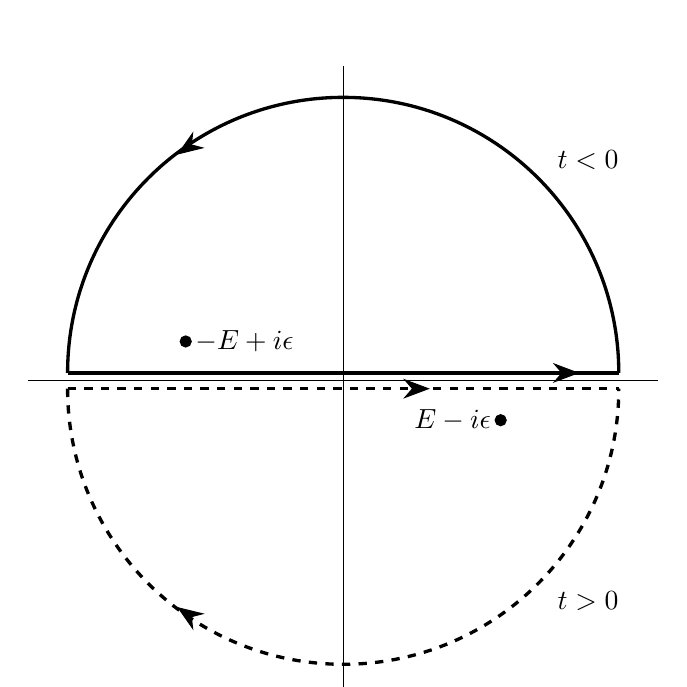
\begin{tikzpicture}
    \draw[very thick] (-3.5,0.1) -- (3.5,0.1);
    \draw [-{Stealth[scale=2]}] (2.9,0.1) -- (3,0.1);
    \draw [-{Stealth[scale=2]}] (1,-0.1) -- (1.1,-0.1);
    \draw (2.6,2.8) node[anchor=west]{$t<0$};
    \draw[very thick,dashed] (-3.5,-0.1) -- (3.5,-0.1);
    \draw (2.6,-2.8) node[anchor=west]{$t>0$};
    \draw (0,-4) -- (0,4);
    \draw (-4,0) -- (4,0);
    \draw[very thick] (3.5,0.1) arc (0:180:3.5);
    \draw[very thick,dashed] (-3.5,-0.1) arc (180:360:3.5);
    \draw [-{Stealth[scale=2]}] (-2.06,2.9065) -- (-2.11,2.8723);
    \draw [-{Stealth[scale=2]}] (-2.06,-2.9065) -- (-2.11,-2.8723);
    \filldraw (2,-0.5) circle (2pt) node[anchor=east]{$E-i\epsilon$};
    \filldraw (-2,0.5) circle (2pt) node[anchor=west]{$-E+i\epsilon$};
  \end{tikzpicture}
  \caption{The contour to be used for $\int dk^0\, \frac{e^{-ik_0t}}{k_0^2-A^2-i\epsilon}$ depending on whether $t>0$ or $t<0$.}
  \label{fig:epsilon-complex-plane}
\end{figure}

We can now use $I$ to solve (\ref{eqn:2pcf-integral-halfway}). Dropping proportionality constants which do not matter for this demonstration, and assuming $x>0$ and $t>0$,
\begin{es}
  \braket{0|\hat\phi(x)\hat\phi(0)|0} &\propto\int d^3 \bm k\, \frac{e^{i(xk_1 - t\sqrt{\bm k^2+ m^2})}}{\sqrt{\bm k^2+ m^2}}\\
  &=\int dk_2 dk_3\int dk_1\, \frac{e^{i(xk_1 - t\sqrt{k_1^2+ F^2})}}{\sqrt{k_1^2+F^2}}
\end{es}
where in the second line we defined $F^2 = k_2^2 + k_3^2 + m^2$. We now work on the $k_1$ integral in a similar fashion to the $k_0$ integral. Again, we have poles when the denominator is zero, at $k_1^2 = F^2$, or $k_1 = \pm iF$. But this time there is also a branch cut for all $k_1^2 + F^2 < 0$ due to the difficulty of defining the square root operator on negative real values. The complex plane of this function is depicted in Figure \ref{fig:k1-complex-plane}.

\begin{figure}
  \centering
  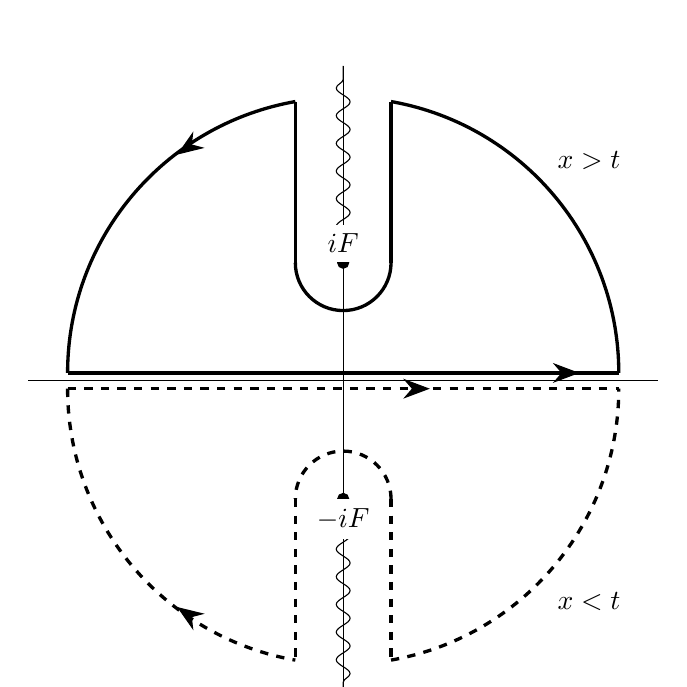
\begin{tikzpicture}
    \draw[very thick] (-3.5,0.1) -- (3.5,0.1);
    \draw [-{Stealth[scale=2]}] (2.9,0.1) -- (3,0.1);
    \draw [-{Stealth[scale=2]}] (1,-0.1) -- (1.1,-0.1);
    \draw (2.6,2.8) node[anchor=west]{$x>t$};
    \draw[very thick,dashed] (-3.5,-0.1) -- (3.5,-0.1);
    \draw (2.6,-2.8) node[anchor=west]{$x<t$};
    \draw (0,-4) -- (0,4);
    \draw (-4,0) -- (4,0);
    \draw[very thick] (3.5,0.1) arc (0:80:3.5);
    \draw[very thick] (-0.6077,3.5468) arc (100:180:3.5);
    \draw[very thick,dashed] (-3.5,-0.1) arc (180:260:3.5);
    \draw[very thick,dashed] (0.6077,-3.5468) arc (280:360:3.5);
    \draw[very thick] (-0.6077,1.5) arc (180:360:0.6077);
    \draw[very thick,dashed] (0.6077,-1.5) arc (0:180:0.6077);
    \draw[very thick] (-0.6077,1.5) -- (-0.6077, 3.5468);
    \draw[very thick] (0.6077,1.5) -- (0.6077, 3.5468);
    \draw[very thick,dashed] (0.6077,-1.5) -- (0.6077, -3.5468);
    \draw[very thick,dashed] (-0.6077,-1.5) -- (-0.6077, -3.5468);

    \path [draw=black,snake it](0,-1.5) -- (0,-4);
    \path [draw=black,snake it](0,1.5) -- (0,4);

    \draw [-{Stealth[scale=2]}] (-2.06,2.9065) -- (-2.11,2.8723);
    \draw [-{Stealth[scale=2]}] (-2.06,-2.9065) -- (-2.11,-2.8723);
    \filldraw (0,1.5) circle (2pt) node[anchor=south, fill=white]{$iF$};
    \filldraw (0,-1.5) circle (2pt) node[anchor=north, fill=white]{$-iF$};
  \end{tikzpicture}
  \caption{The contour to be used for $\int dk_1\, \frac{e^{i(xk_1 - t\sqrt{k_1^2+ F^2})}}{\sqrt{k_1^2+F^2}}$, with the branch cut.}
  \label{fig:k1-complex-plane}
\end{figure}

To work out whether to close the contour above or below the real line, we substitute $k_1 = Re^{i\theta}$ into the exponent, leaving a real part of $-R\sin\theta(x - t)$. We close the contour in the region where this real part is small, which is above the real line for $x>t$ and below it for $x<t$. However, we must avoid the branch cut by looping the contour around it, which adds nonzero values where the contour nears the origin. The scale of this added amount is controlled by the value of the integrand near the end of the branch cut, where the integrand is largest. For $x>t$, this occurs for $k_1 = i(F - \delta)$ with $\delta$ small, and the integrand is
\begin{e}
  \sim\frac{e^{-xF}}{\sqrt{2F\delta}}.
\end{e}
Meanwhile, for $x<t$, the integrand near $k_1 = -i(F - \delta)$ is considerably larger:
\begin{e}
  \sim\frac{e^{xF}}{\sqrt{2F\delta}}.
\end{e}
It follows that the 2PCF is nonzero for $x<t$, which is inside the lightcone. But when the lightcone and correlations are forbidden by causality, the 2PCF decays exponentially. This is reminiscent of how a wavefunction decreases exponentially in a region where potential energy is greater than the energy of the particle in non-relativistic quantum mechanics, or of how a light wave exponentially decays in a medium which cannot support its frequency. Thus, the QFT principle of least action not only obeys causality, but does so in a manner similar to both quantum mechanical and classical field theories.

The exponential decrease outside the lightcone came from our choice to add $i\epsilon$ to the denominator of the Green's function. This shifted the $\pm E$ poles above and below the real line as shown in Figure \ref{fig:epsilon-complex-plane}. If we had shifted the poles in another way, we would not have gotten the cancellation we achieved, and the 2PCF would not have fallen outside the light cone. This choice of pole-shifting was made by Richard Feynman and is known as the \emphi{Feynman Propagator}, and we will nearly always use it in the future.

Due to the success of the QFT principle of least action in this free scalar field case, we are inspired to continue on to the $\lambda \neq 0$ case of an interacting theory, which contains a vast variety of novel phenomena.


\section{Solving the Spin Zero Path Integral With Interactions}

One of the key results of the previous section was that for a non-interacting theory where the Lagrangian density is Gaussian, particles cannot transfer momenta and cannot scatter. The proof of this is (\ref{eqn:separable-gaussian-lagrangian}), where we separated an $2n$PCF attained by Wick's theorem into $n$ multiplied factors, each of which enforced momentum conservation.

However, real particles scatter, so to make a true particle theory we will have to break the chain of logic that led us to the no-scattering conclusion. The solution is to add a small, non-quadratic term to the Lagrangian density, which adds small additional terms to the $2n$PCF which are not separable. These small terms allow a small amount of momentum transfer between the $n$ particles, causing scattering. This is the motivation for us associating the $\frac{\lambda}{4!}\phi^4$ term in $\mathcal{L}$ with scattering. In this section, we'll compute the effect of this new term on the momentum-space $n$PCFs.

Our strategy will be to apply the momentum-transferring $\phi^4$ term as a perturbation to the Gaussian free theory discussed above. In other words, we'll write
\begin{ec}
  S = S_0 + \lambda S_1,\\
  \qquad S_0 = \int d^4 x\, \parens{\frac{1}{2}(\del_\mu \phi)^2 - \frac{1}{2}m^2 \phi^2},\qquad S_1 = -\int d^4x\, \frac{1}{4!}\phi^4
  \label{eqn:perturbation-actions}
\end{ec}
Our goal will be to produce a power series in $\lambda$ for $n$PCFs, of which the zeroth order term is (\ref{eqn:scalar-theory-npcf}) and the following terms are small momentum-mixing terms under the assumption that $\lambda \ll 1$. To do this, we start with the QFT principle of least action:
\begin{e}
  \braket{0|\hat\phi(x_1)\cdots\hat\phi(x_n)|0} = \frac{\int \mathcal{D}\phi\, \phi(x_1)\cdots\phi(x_n)e^{iS_0 + i\lambda S_1}}{\int \mathcal{D}\phi\,e^{iS_0 + i\lambda S_1}}.
\end{e}
Obtaining a power series in $\lambda$ is just as simple as expanding the exponent as a power series:
\begin{e}
  \braket{0|\hat\phi(x_1)\cdots\hat\phi(x_n)|0} = \frac{\int \mathcal{D}\phi\, \phi(x_1)\cdots\phi(x_n)e^{iS_0}\parens{1 + i\lambda S_1 - \frac{\lambda^2}{2} S_1^2 + \dots}}{\int \mathcal{D}\phi\,e^{iS_0}\parens{1 + i\lambda S_1 - \frac{\lambda^2}{2} S_1^2 + \dots}}.
  \label{eqn:interacting-scalar-partway}
\end{e}
Now that only the quadratic term $S_0$ remains in the exponent of the integrand, (\ref{eqn:interacting-scalar-partway}) can be completely solved to arbitrary order with Wick's theorem! For example, when $S_1$ as defined in (\ref{eqn:perturbation-actions}) is substituted into the above equation, the numerator expands to
\begin{ec}
  \int \mathcal{D}\phi\, \phi(x_1)\cdots\phi(x_n)e^{iS_0} \\- \frac{i\lambda}{4!} \int d^4 x \int \mathcal{D}\phi\, \phi(x_1)\cdots\phi(x_n)e^{iS_0}\phi^*(x)\phi(x)\phi^*(x)\phi(x) + \mathcal{O}(\lambda^2).
  \label{eqn:first-order-npcf}
\end{ec}
Both of these terms are Gaussian correlation functions. The first line is the same $n$PCF we found for the non-interacting theory, confirming our expectation that adding the small $\phi^4$ perturbation did not change the first-order structure of the theory. The second is an $n+4$PCFs which will allow these $n$ particles to interact and exchange momentum.

To see this momentum exchange clearly, we will switch to the momentum basis. Fortunately, the hard work of determining how $n$PCFs Fourier transform was done in (\ref{eqn:scalar-theory-npcf}), which reduced a momentum-space $n$PCF to products of Greens functions evaluated on Wick contractions of $\phi$s. The only trickiness introduced by interactions is the fact that the $\phi(x)$s that come from the perturbation $S_1$ are integrated over, as in the second line of (\ref{eqn:first-order-npcf}). This position integral becomes
\begin{es}
  \int d^4 x \braket{\hat \phi(x)^4} &= \int d^4 x \int \ftve{4}{k_1}\dots \ftve{4}{k_4}e^{ik_1\cdot x}\dots e^{ik_4\cdot x}\braket{\hat \phi(k_1)\dots \phi(k_4)}\\
  &= \int d^4 x \int \ftve{4}{k_1}\dots \ftve{4}{k_4}e^{i(k_1+\dots+k_4)\cdot x}\braket{\hat \phi(k_1)\dots \phi(k_4)}\\
  &= \int \ftve{4}{k_1}\dots \ftve{4}{k_4}\delta(k_1+\dots+k_4)\braket{\hat \phi(k_1)\dots \phi(k_4)}.
  \label{eqn:momentum-conservation-at-vertex}
\end{es}
In other words, when some of the $x$ values of an $n$PCF are the same in position space, then the corresponding $k$ values in the momentum space have to sum to zero. This mathematical fact looks similar to momentum conservation, and in fact we'll see in the next section that (\ref{eqn:momentum-conservation-at-vertex}) does enforce momentum conservation in scattering events.

In principle, we have now computed an interacting theory $n$PCF. (\ref{eqn:interacting-scalar-partway}) describes how to use perturbation theory to write an interacting $n$PCF in terms of non-interacting $m$PCFs We computed these $m$PCFs in (\ref{eqn:scalar-theory-npcf}) using Wick's theorem, and (\ref{eqn:momentum-conservation-at-vertex}) describes how to integrate over the $\phi$ values present in the perturbing action $S_1$. Actually using these formulas however is a complicated and error-prone task. Fortunately, there is a graphical technique to isolate the Wick pairs and reduce these three equations to one simple form. This technique is called a Feynman diagram, introduced by Richard Feynman in the 1960s, and is widely used across high energy physics.


\subsection{Feynman Diagrams}

To compute an $n$PCF in momentum space, (\ref{eqn:scalar-theory-npcf}) dictates that we must contract the $\hat \phi$ operators into pairs. The goal of a Feynman diagram is to do this visually. Let's represent every point in spacetime as a vertex in a graph, and Wick contractions are represented as edges (called propagators) between the vertices. In an interacting theory, some of the vertices come from the original $n$PCF to be computed. These vertices were denoted as $k_i$ and are called \emphi{external vertices}. Others, called \emphi{internal vertices}, come from the perturbation $S_1$ and will be integrated over. Because each external vertex only has one $\phi$ operator attached to it, they will only connect to one edge. Each internal vertex will connect to four edges because every $S_1$ term contains four $\phi$s each, due to the $\phi^4$ of the Lagrangian.

After the propagators are drawn in according to these rules, we can assign momentum values to the $\phi$ terms. Each Wick contraction consists of two operators $\phi(k_1)\phi(k_2)$ which may have different momenta. However, (\ref{eqn:scalar-theory-npcf}) showed that if $k_1 \neq k_2$, then the entire diagram will evaluate to zero. Thus, we can assume that $k_1 = k_2 = k$. As shorthand, we assign a momentum of $k$ to the propagator that represents this Wick contraction.

% \begin{figure}
%   \centering
%   \begin{tikzpicture}
%     \draw (-4.5,0) node {$\mathcal{O}(\lambda)=$};
%     \filldraw[black] (-3,0) circle (2pt);
%     \draw (-2.4,0.2) node[anchor=south] {$p$};
%     \draw[-stealth] (-2.8,0.1) -> (-2.2,0.1);
%     \draw (-1.6,0.2) node[anchor=south] {$q$};
%     \draw[-stealth] (-1.8,0.1) -> (-1.2,0.1);
%     \filldraw[black] (-1,0) circle (2pt);
%     \draw (-2,0) circle (2pt);
%     \draw (-3,0) -- (-1,0);
%     \draw[black] (-2,-0.3) circle (0.3);
%     \draw[black] (-2,1.4) node[anchor=north] {(1)};
%     \draw (-2,-0.8) node[anchor=north] {$k$};
%     \draw[-stealth] (-2.3,-0.7) -> (-1.7,-0.7);

%     \draw[black] (0,0) node {$+$};

%     \filldraw[black] (1,0) circle (2pt);
%     \filldraw[black] (3,0) circle (2pt);
%     \draw[-stealth] (0.9,0.3) -> (1.4,0.8);
%     \draw (1.2,0.6) node[anchor=east] {$p$};
%     \draw[-stealth] (2.6,0.8) -> (3.1,0.3);
%     \draw (2.8,0.6) node[anchor=west] {$q$};
%     \draw (2,0) circle (2pt);
%     \draw (1,0) arc (165:15:1.05);
%     \draw[black] (2,-0.3) circle (0.3);
%     \draw[black] (2,0.3) circle (0.3);
%     \draw[black] (2,1.4) node[anchor=north] {(2)};
%     \draw[-stealth] (1.6,0.5) -> (1.6,0.0);
%     \draw[black] (1.7,0) node[anchor=north east] {$k_1$};
%     \draw[-stealth] (2.4,-0.5) -> (2.4,0.0);
%     \draw[black] (2.4,0) node[anchor=north west] {$k_2$};
%   \end{tikzpicture}
%   \caption{Feynman diagrams for a $2$PCF in the interacting scalar theory. Each line is a Wick pair and each vertex is a point in spacetime.}
%   \label{fig:feynman-construction}
% \end{figure}


\begin{figure}
  \centering
  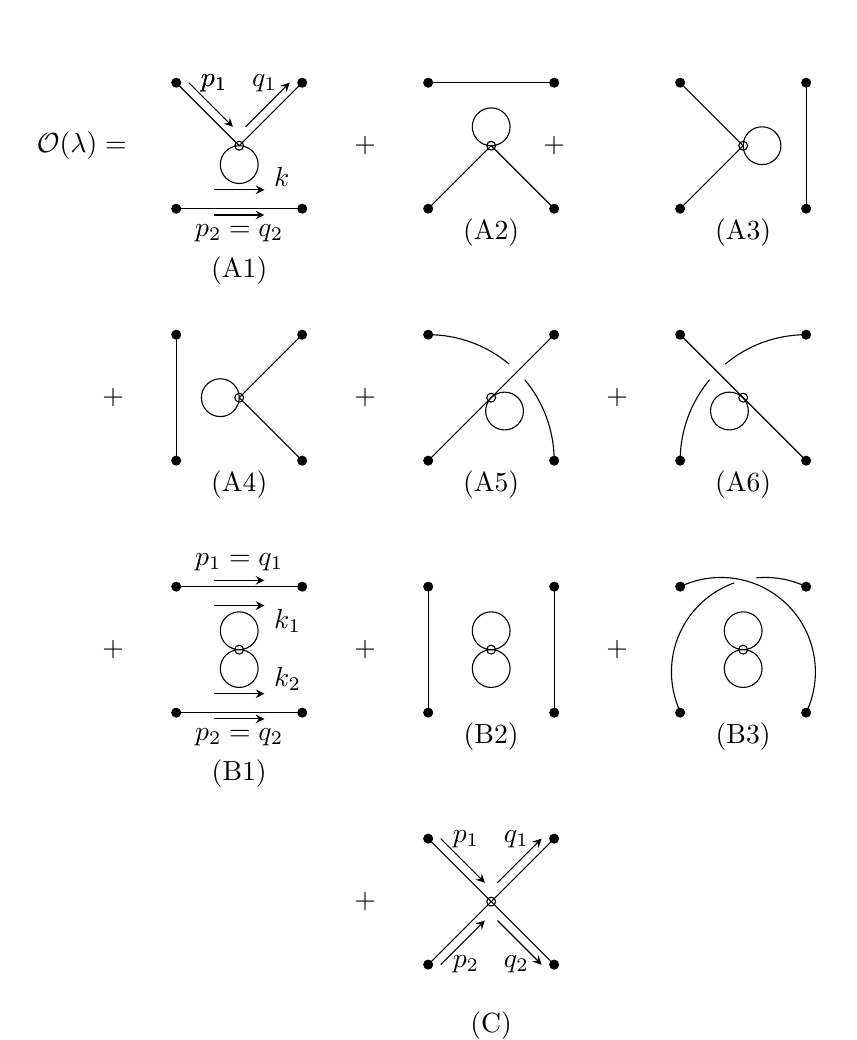
\begin{tikzpicture}[scale=0.8]
    \draw (-4.5,0) node {$\mathcal{O}(\lambda)=$};
    \filldraw (-3,1) circle (2pt);
    \filldraw (-1,1) circle (2pt);
    \filldraw (-1,-1) circle (2pt);
    \filldraw (-3,-1) circle (2pt);
    \draw (-2,0) circle (2pt);
    \draw (-2, -1.6) node[anchor=north] {(A1)};
    \draw (-3,1) -- (-2,0);
    \draw (-1,1) -- (-2,0);
    \draw (-1,-1) -- (-3,-1);
    \draw (-2, -0.3) circle (0.3);
    \draw[-stealth] (-2.8,1) -- (-2.1,0.3);
    \draw[stealth-] (-1.2,1) -- (-1.9,0.3);
    \draw (-1.6,0.7) node[anchor=south] {$q_1$};
    \draw (-2.4,0.7) node[anchor=south] {$p_1$};
    \draw[-stealth] (-2.4,-1.1) -- (-1.6,-1.1);
    \draw (-2,-1.1) node[anchor=north] {$p_2=q_2$};
    \draw (-2.4,0.7) node[anchor=south] {$p_1$};
    \draw[-stealth] (-2.4,-0.7) -- (-1.6,-0.7);
    \draw (-1.6,-0.8) node[anchor=south west] {$k$};
    
    \draw (0,0) node {$+$};

    \filldraw (3,1) circle (2pt);
    \filldraw (1,1) circle (2pt);
    \filldraw (1,-1) circle (2pt);
    \filldraw (3,-1) circle (2pt);
    \draw (2,0) circle (2pt);
    \draw (2, -1) node[anchor=north] {(A2)};
    \draw (3,-1) -- (2,0);
    \draw (1,-1) -- (2,0);
    \draw (1,1) -- (3,1);
    \draw (2, 0.3) circle (0.3);

    \draw (3,0) node {$+$};

    \filldraw (7,1) circle (2pt);
    \filldraw (5,1) circle (2pt);
    \filldraw (5,-1) circle (2pt);
    \filldraw (7,-1) circle (2pt);
    \draw (6,0) circle (2pt);
    \draw (6, -1) node[anchor=north] {(A3)};
    \draw (5,-1) -- (6,0);
    \draw (5,1) -- (6,0);
    \draw (7,1) -- (7,-1);
    \draw (6.3, 0) circle (0.3);

    \draw (-4,-4) node {$+$};

    \filldraw (-3,-3) circle (2pt);
    \filldraw (-1,-3) circle (2pt);
    \filldraw (-1,-5) circle (2pt);
    \filldraw (-3,-5) circle (2pt);
    \draw (-2,-4) circle (2pt);
    \draw (-2, -5) node[anchor=north] {(A4)};
    \draw (-1,-5) -- (-2,-4);
    \draw (-1,-3) -- (-2,-4);
    \draw (-3,-3) -- (-3,-5);
    \draw (-2.3, -4) circle (0.3);

    \draw (0,-4) node {$+$};

    \filldraw (1,-3) circle (2pt);
    \filldraw (3,-3) circle (2pt);
    \filldraw (3,-5) circle (2pt);
    \filldraw (1,-5) circle (2pt);
    \draw (2,-4) circle (2pt);
    \draw (2, -5) node[anchor=north] {(A5)};
    \draw (3,-3) -- (1,-5);
    \draw (2.212, -4.212) circle (0.3);
    \draw (3,-5) arc (0:40:2);
    \draw (2.28557521937,-3.46791111376) arc (50:90:2);

    \draw (4,-4) node {$+$};

    \filldraw (5,-3) circle (2pt);
    \filldraw (7,-3) circle (2pt);
    \filldraw (7,-5) circle (2pt);
    \filldraw (5,-5) circle (2pt);
    \draw (6,-4) circle (2pt);
    \draw (6, -5) node[anchor=north] {(A6)};
    \draw (5,-3) -- (7,-5);
    \draw (5.782, -4.212) circle (0.3);
    \draw (7,-3) arc (90:130:2);
    \draw (5.46791111376,-3.71442478063) arc (140:180:2);

    \draw (-4,-8) node {$+$};

    \filldraw (-3,-7) circle (2pt);
    \filldraw (-1,-7) circle (2pt);
    \filldraw (-1,-9) circle (2pt);
    \filldraw (-3,-9) circle (2pt);
    \draw (-2,-8) circle (2pt);
    \draw (-2, -9.6) node[anchor=north] {(B1)};
    \draw (-1,-7) -- (-3,-7);
    \draw (-1,-9) -- (-3,-9);
    \draw (-2, -8.3) circle (0.3);
    \draw (-2, -7.7) circle (0.3);
    \draw[-stealth] (-2.4, -6.9) -- (-1.6, -6.9);
    \draw[-stealth] (-2.4, -7.3) -- (-1.6, -7.3);
    \draw[-stealth] (-2.4, -8.7) -- (-1.6, -8.7);
    \draw[-stealth] (-2.4, -9.1) -- (-1.6, -9.1);
    \draw (-2,-6.9) node[anchor=south] {$p_1=q_1$};
    \draw (-1.6,-7.2) node[anchor=north west] {$k_1$};
    \draw (-1.6,-8.8) node[anchor=south west] {$k_2$};
    \draw (-2,-9.1) node[anchor=north] {$p_2=q_2$};

    \draw (0,-8) node {$+$};

    \filldraw (3,-7) circle (2pt);
    \filldraw (1,-7) circle (2pt);
    \filldraw (1,-9) circle (2pt);
    \filldraw (3,-9) circle (2pt);
    \draw (2,-8) circle (2pt);
    \draw (2, -9) node[anchor=north] {(B2)};
    \draw (1,-7) -- (1,-9);
    \draw (3,-7) -- (3,-9);
    \draw (2, -8.3) circle (0.3);
    \draw (2, -7.7) circle (0.3);

    \draw (4,-8) node {$+$};

    \filldraw (7,-7) circle (2pt);
    \filldraw (5,-7) circle (2pt);
    \filldraw (5,-9) circle (2pt);
    \filldraw (7,-9) circle (2pt);
    \draw (6,-8) circle (2pt);
    \draw (6, -9) node[anchor=north] {(B3)};
    \draw (6, -8.3) circle (0.3);
    \draw (6, -7.7) circle (0.3);
    \draw (7, -9) arc (-25.5287793655:115.528779366:1.5);
    \draw (7, -7) arc (64.4712206345:95.633022225:1.5);
    \draw (5.85754508895, -6.94075745063) arc (109.633022225:205.528779366:1.5);

    \draw (0,-12) node {$+$};

    \filldraw (1,-11) circle (2pt);
    \filldraw (3,-11) circle (2pt);
    \filldraw (3,-13) circle (2pt);
    \filldraw (1,-13) circle (2pt);
    \draw (2,-12) circle (2pt);
    \draw (2, -13.6) node[anchor=north] {(C)};
    \draw (3,-11) -- (1,-13);
    \draw (3,-13) -- (1,-11);
    \draw[stealth-] (2.8,-11) -- (2.1,-11.7);
    \draw[-stealth] (1.2,-11) -- (1.9,-11.7);
    \draw[stealth-] (2.8,-13) -- (2.1,-12.3);
    \draw[-stealth] (1.2,-13) -- (1.9,-12.3);
    \draw (1.6,-11.3) node[anchor=south] {$p_1$};
    \draw (2.4,-11.3) node[anchor=south] {$q_1$};
    \draw (1.6,-12.7) node[anchor=north] {$p_2$};
    \draw (2.4,-12.7) node[anchor=north] {$q_2$};

  \end{tikzpicture}
  \caption{Feynman diagrams for a $4$PCF $\braket{\hat \phi(p_1)\hat \phi(p_2) \hat \phi(q_1) \hat \phi(q_2)}$ in the interacting scalar theory. Each line is a Wick pair and each vertex is a point in spacetime.}
  \label{fig:feynman-construction}
\end{figure}

For a 4PCF in the scalar interacting theory there are four external vertices. There is one internal vertex to first order in $\lambda$. Following the rules for drawing edges, there are ten ways of pairing the $\phi$s to evaluate the numerator of (\ref{eqn:interacting-scalar-partway}) which are shown in Figure \ref{fig:feynman-construction}. Diagrams A1-A6 are similar, as are B1-B3, so we will only calculate one diagram from each of these classes. For this reason, only the momenta of this diagram are labeled. The direction in which momentum is chosen to flow is a matter of preference.

To calculate the 4PCF $\braket{\hat \phi(p_1)\hat \phi(p_2) \hat \phi(q_1) \hat \phi(q_2)}$ from a diagram, we follow (\ref{eqn:scalar-theory-npcf}) by writing $G(k)$ for every propagator with momentum $k$. For internal vertices, (\ref{eqn:momentum-conservation-at-vertex}) tells us to enforce momentum conservation by integrating over all momenta subject to the constraint that the total momentum of all the propagators connected to an internal vertex is zero. Thus diagram A1 diagrams evaluates to 
\begin{es}
  \mathrm{(A1)} &\propto G(p_1) G(q_1)G(p_2)\delta(p_2-q_2) \int \ftve{4}{k} \delta(p_1 - q_1 + k - k)G(k)\\
   &\propto G(p_1) G(q_1) \delta(p_1 - q_1)\delta(p_2-q_2)\int \ftve{4}{k} G(k).\\
  \label{eqn:scattering-diagram-a}
\end{es}
The proportionality statements acknowledge that we are focusing on the structure of the Green's functions and have not yet put in the correct powers of $\lambda$ or other coefficients that might appear.

The first delta function in line 1 is the delta function of (\ref{eqn:scalar-theory-npcf}), enforcing that momentum does not change along a propagator. The second delta function is the delta function of  (\ref{eqn:momentum-conservation-at-vertex}), enforcing that momentum cannot change at a vertex. For this diagram, these constraints together enforce that momentum of each must be conserved, and the double $\delta$-function in the above equation falls out to prevent the momenta from being mixed. That is, the free theory did not lead to momentum mixing in this case. It only changed the value of the 4PCF by some value $\int \ftve{4}{k} G(k)$ which we have not computed yet.

We can compute the diagrams (B1) and (C) in a similar way:
\begin{es}
  \mathrm{(B1)} &\propto G(p_1)\delta(p_1-q_1) G(p_2)\delta(p_2-q_2)\int \ftve{4}{k_1}\ftve{4}{k_2}G(k_1)G(k_2)\\
  \mathrm{(C)} &\propto G(p_1)G(p_2)G(q_1)G(q_2)\delta(p_1+p_2+q_1+q_2).
  \label{eqn:scattering-diagrams-b-c}
\end{es}

Diagram (B1) is like A1 in that it conserves momentum for each pair of particles. However, Diagram (C) allows the much-heralded momentum mixing. Even if $p_1$, $p_2$, $q_1$, and $q_2$ are all different, (C) will be nonzero as long as the momenta sum to zero. This diagram (and only this diagram) is the leading order contribution to $\phi\phi\rightarrow\phi\phi$ scattering, and we will use it a great deal throughout the rest of this chapter.

We have now verified that this $\phi^4$ theory allows particles to interact. Before moving on to quantify this interaction by computing scattering cross sections, it's worth covering two more details. The first is to replace the above two proportionality statements with actual equations. The second is to work out the denominator of (\ref{eqn:interacting-scalar-partway}) and divide the sum of the (A), (B), and (C) diagrams by that to have a full equation for the interacting theory $n$PCF.

\subsection{Symmetry Factor and Feynman Rules}
All of the diagrams drawn in figure \ref{fig:feynman-construction} were first order, since they contained only one power of $S_1$ and therefore only one power of $\lambda$. If we had written the diagrams of order $\lambda^2$, they would have had two internal vertices (one for each $S_1$). Thus, every diagram should be multiplied by the constant $i\lambda$ for every internal vertex.

Another potential worry is the possibility of under-counting. $S_1$ contains four $\phi$s, which can each be contracted with another $\phi$ in the $n$PCF. Contracting with the first $\phi$ and contracting with the second represent different contractions and should be added individually. But this is not reflected in our Feynman diagram, where we draw a contraction with any one of the $\phi$s as a propagator running into the internal vertex and make no note of which $\phi$ it was contracted with. Another source of error enters when we compute second order diagrams: these involve two identical $S_1$ values connected in different ways to the exterior vertices. We should double each diagram to reflect the fact that the two $S_1$ values could be swapped without changing the diagram structure. There are more numerical factors we haven't taken care of as well, which are all represented in table \ref{tab:symmetry-factor}.

\begin{table}
  \centering
  \bgroup
  \small
  \def\arraystretch{3}
  \begin{tabular}{c|c}
    \hline \hline
    Contribution & Source\\ \hline
    $\displaystyle \frac{(-i\lambda)^n}{n!}$ & Taylor series expansion of $e^{-iS_1}$\\
    $\displaystyle \frac{1}{4!}$ & Definition of the interacting term in the Lagrangian\\
    $n!$ & The number of ways to swap internal vertices\\
    $\displaystyle \frac{1}{(\mathrm{identical\ vertices})!}$ & \makecell{In the above row, we should not have swapped \\vertices which were already identical in the diagram}\\
    $4!$ & \makecell{The number of ways to connect 4 $\phi$s to 4 incoming\\ propagators for each internal vertex}\\
    $\displaystyle \frac{1}{2^{\mathrm{reversible\ propagators}}}$ & \makecell{In the above row, we should not have \\swapped propagators that both came \\from and led to the same vertex}\\
    \hline \hline
  \end{tabular}
  \caption{Factors we should multiply each Feynman diagram by due to expansion coefficients, over- or under-counting, and other sources. Here, $n$ represents the number of internal vertices.}
  \egroup
  \label{tab:symmetry-factor}
\end{table}

To get the total correction to each diagram, we multiply every entry in the left hand column of table \ref{tab:symmetry-factor}. Most of the entries cancel, but to keep track of those that don't, we define the \emphi{symmetry factor}
\begin{e}
  S_f = (1+\mathrm{identical\ vertices})!(1+\mathrm{reversible\ propagators})!
  \label{eqn:symmetry-factor}
\end{e}
where identical vertices are internal vertices which are connected to the same vertices as each other, and reversible propagators are those that lead to and out of the same internal vertex.
in which case we should multiply each diagram by the factor $(-i\lambda)^n / S_f$.

As an example, in figure \ref{fig:feynman-construction}, all the A diagrams have symmetry factor 2 due to the reversible propagator with momentum $k$. The B diagrams have symmetry factor 4 because they have two reversible propagators, and the C diagram has symmetry factor 1 because there are no reversible propagators or identical vertices.

The definition of the symmetry factor allows us to write down the value of any diagram exactly by following the following rules, called the \emphi{Feynman rules}:
\begin{enumerate}
  \item The edge \raisebox{0.2em}{\begin{tikzpicture}[scale=0.8]
    \draw (-0.7,0) -- (0.7,0);
    \draw[-stealth] (-0.3,0.1) -- (0.3,0.1);
    \draw (-0,0.1) node[anchor=south]{$k$};
  \end{tikzpicture}} contributes $G(k)$
  \item A vertex \raisebox{-2.3em}{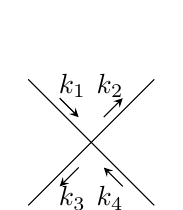
\begin{tikzpicture}[scale=0.8]
    \draw (-1,1) -- (1,-1);
    \draw (-1,-1) -- (1,1);
    \draw[-stealth] (-0.5,0.7) -- (-0.2,0.4);
    \draw (-0.3,0.55) node[anchor=south]{$k_1$};
    \draw[stealth-] (0.5,0.7) -- (0.2,0.4);
    \draw (0.3,0.55) node[anchor=south]{$k_2$};
    \draw[stealth-] (-0.5,-0.7) -- (-0.2,-0.4);
    \draw (-0.3,-0.55) node[anchor=north]{$k_3$};
    \draw[-stealth] (0.5,-0.7) -- (0.2,-0.4);
    \draw (0.3,-0.55) node[anchor=north]{$k_4$};
  \end{tikzpicture}} contributes $-i\lambda \delta(k_1 - k_2 - k_3 + k_4)$
  \item Every internal propagator $k$ is integrated over $\int \ftve{4}{k}$
  \item Diagrams with exchangeable vertices or reversible edges contribute a symmetry factor $S_f$.
\end{enumerate}

Once the diagrams are computed, they may be added and the sum divided by the denominator of (\ref{eqn:interacting-scalar-partway}), discussed in the next section, to get the $n$PCF

% \begin{figure}
%   \centering
%   \begin{tikzpicture}[scale=0.8]
%     \draw (-6.8,0) node {$\mathcal{O}(\lambda^2)=$};
%     \draw[black] (-5,0) node[anchor=east] {$x_1$};
%     \draw[black] (-3,0) node[anchor=west] {$x_2$};
%     \draw (-5,0) -- (-3,0);
%     \draw[black] (-3.7,-0.3) circle (0.3);
%     \draw[black] (-4.3,0.3) circle (0.3);

%     \draw (-2,0) node {$+$};

%     \draw[black] (-1,0) node[anchor=east] {$x_1$};
%     \draw[black] (1,0) node[anchor=west] {$x_2$};
%     \draw (-1,0) -- (1,0);
%     \draw[black] (0,-0.3) circle (0.3);
%     \draw[black] (0,-0.9) circle (0.3);
    
%     \draw (2,0) node {$+$};

%     \draw[black] (3,0) node[anchor=east] {$x_1$};
%     \draw[black] (5,0) node[anchor=west] {$x_2$};
%     \draw[black] (4,0) circle (0.5);
%     \draw (3,0) -- (5,0);

%     \draw (-6,-3) node {$+$};

%     \draw[black] (-5,-3) node[anchor=east] {$x_1$};
%     \draw[black] (-3,-3) node[anchor=west] {$x_2$};
%     \draw[black] (-3.6,-3) circle (0.3);
%     \draw[black] (-3.6,-3.6) circle (0.3);
%     \draw[black] (-4.4,-3) circle (0.3);
%     \draw[black] (-4.4,-3.6) circle (0.3);
%     \draw (-5,-3) arc (165:15:1.05);
   
%     \draw (-2,-3) node {$+$};

%     \draw[black] (-1,-3) node[anchor=east] {$x_1$};
%     \draw[black] (1,-3) node[anchor=west] {$x_2$};
%     \draw[black] (-0.6,-3.4) circle (0.3);
%     \draw[black] (-0,-3.4) circle (0.3);
%     \draw[black] (0.6,-3.4) circle (0.3);
%     \draw (-1,-3) arc (165:15:1.05);

%     \draw (2,-3) node {$+$};

%     \draw[black] (3,-3) node[anchor=east] {$x_1$};
%     \draw[black] (5,-3) node[anchor=west] {$x_2$};
%     \draw[black] (4,-3.4) circle (0.5);
%     \draw[black] (3.5,-3.4) -- (4.5, -3.4);
%     \draw (3,-3) arc (165:15:1.05);

%     \draw (-2,-6) node {$+$};

%     \draw[black] (-1,-6) node[anchor=east] {$x_1$};
%     \draw[black] (1,-6) node[anchor=west] {$x_2$};
%     \draw[black] (-0.3,-6.4) circle (0.3);
%     \draw[black] (0.3,-6.4) circle (0.3);
%     \draw[black] (0,-5.53) circle (0.3);
%     \draw (-1,-6) arc (165:15:1.05);
%   \end{tikzpicture}
%   \caption{Second order Feynman diagrams for the $\phi^4$ theory.}
%   \label{fig:feynman-second-order}
% \end{figure}


\subsection{The Denominator: Vacuum Diagram Cancellation}
This section deals with the denominator of (\ref{eqn:interacting-scalar-partway}):
$$\int \mathcal{D}\phi e^{-i S_0}e^{-iS_1}$$
which we must divide the sum of all Feynman diagrams by to get an $n$PCF. This factor came from requiring the $n$PCF to be normalized. Fortunately, this integral will cancel perfectly with terms in the numerator.

To see how, consider the diagrammatic expansion of this denominator. It is essentially a 0PCF, if such a thing exists. For scalar field theory, the zeroth order term is 1 and the the first order diagram is
\begin{center}
  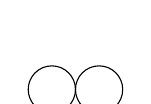
\begin{tikzpicture}
    \draw (-0.3,0) circle(0.3);
    \draw (0.3,0) circle(0.3);
  \end{tikzpicture}
\end{center}
where we have left out the circle to indicate the internal vertex (this is often done since any intersection of propagators is clearly a vertex).

This kind of diagram which is unconnected to external vertices called a \emphi{vacuum diagram}. You may recognize it diagram as a part of all the (B) diagrams in figure \ref{fig:feynman-construction}. In fact, the vacuum diagrams in the denominator will cancel with all of the diagrams in the numerator like (B) that have vacuum sub-diagrams. The mathematical explanation for this fact is that for every diagram like (A) or (C) that has no vacuum sub-diagrams, you can just multiply by a vacuum sub-diagram to get a diagram like (B), where both are combined. The reverse of this statement is that to divide by the vacuum diagrams, we need to remove all the diagrams like (B) that have vacuum sub-diagrams.

There is also physical intuition for removing by diagrams like (B) that have vacuum sub-diagrams. The vacuum diagrams have no external vertices, and external vertices generally represent particles. Thus, vacuum diagrams represent some change in energy of the vacuum, hence the name. Changes to the vacuum energy are generally undetectable, since we can only measure energy differences between systems and the vacuum is always present. For this reason, we should not count diagrams like (B) that measure the energy of the vacuum.\footnote{This is fortunate for us, since the vacuum diagrams can be infinite. The internal vertices come with integrals over momenta due to the Feynman rules, but the lack of external vertices gives fewer delta functions. For many internal vertices, the diagrams can blow up.}

Now that we know not to draw diagrams with vacuum sub-diagrams, we can fully compute any $n$PCF in the interacting theory with the Feynman rules. Our first and primary application for this newfound power will be to compute scattering amplitudes, which the next section is devoted to.

\section{Spin Zero Scattering}
\label{sec:spin-zero-scattering}
In this section, we'll compute scattering amplitudes for $\phi\phi \rightarrow \phi\phi$ and $\phi \rightarrow \phi\phi\phi$ to get used to $\phi^4$ theory and to practice with the Feynman rules. We'll follow up with a theory of two scalar particles and compute the probability of decay between the two.

Chapter \ref{chap:scattering} informed us that the scattering probability is the square of the $S$ matrix, where the $S$ matrix entry for $m$ particles with momenta $p_i$ scattering to $n$ particles with momenta $-q_i$is given by the $(m+n)$PCF for momenta $p_i$ and $q_i$. We noted however that the $S$ matrix is mostly zero; only when the incoming total momentum equals the outgoing momentum can scattering occur. This appeared in our calculation in the previous section of the 4PCF as well: every diagram in (\ref{eqn:scattering-diagram-a}) and (\ref{eqn:scattering-diagrams-b-c}) was multiplied by $\delta(p_1 + p_2 + q_1 + q_2)$.

We stripped off this delta function part by defining the scattering amplitude $-iM$ as the part of the $S$ matrix with $p_1 + p_2 + q_1 + q_2=0$, but excluding the no-scattering, diagonal entries where $p_1 = p_2$ and $q_1 = q_2$. The (A) diagrams for the 4PCF shown in figure \ref{fig:feynman-construction} had delta functions $\delta(p_1 - p_2)$ and $\delta(q_1-q_2)$, revealing these to be no-scattering diagrams. The only diagram that represents actual $\phi\phi\rightarrow\phi\phi$ scattering to first order is diagram C.

To extract a scattering amplitude from $C$, we must divide the corresponding $n$PCF by the propagator for each incoming and outgoing field, as \jtd{Equation number} dictates. The motivation for this was that we are not interested in the way the particles move before or after they interact, which is represented by the propagators connected to the external legs. We are interested in the actual interaction, which occurs in the middle of diagram (C). Once this division is complete, we get our first ever scattering amplitude:
\begin{e}
  -iM_{\phi\phi \rightarrow \phi \phi} = -i\lambda + \mathcal{O}(\lambda^2).
\end{e}
This equation is very simple, perhaps disappointingly so. Let's calculate the second-order contributions to the scattering amplitude to see if they are more interesting.

The first step is to draw new second-order diagrams. Many of these diagrams will look like this:
\begin{center}
  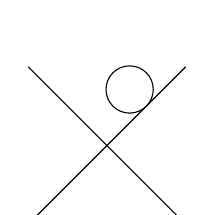
\begin{tikzpicture}
    \draw (-1,1)--(1,-1);
    \draw (-1,-1)--(1,1);
    \draw (0.28786796564, 0.71213203435) circle (0.3);
  \end{tikzpicture}
\end{center}
but these diagrams actually do not contribute to the scattering amplitude. Recall that the point of dividing by $G(p)$ for every external propagator $p$ was to account for the motion of a particle before it interacts. The loop in the above diagram represents particle activity after it has interacted with the rest of the diagram. This loop represents self-interaction and is interesting in its own right. In fact, we'll study it in section \ref{sec:scalar-mass}. However, it still represents a particle propagating on its own and we must divide it out. Therefore, this diagram is just the same $-i\lambda$ first-order diagram we computed above.

This is an example of a generalized rule for calculating scattering amplitudes: the only diagrams that contribute to amplitudes are \emphi{truncated}. The definition of truncated is as follows:
\begin{center}
  \textit{In a truncated diagram, no internal propagators can be cut that sever exactly one external vertex from the diagram.}
\end{center}
An internal propagator is one that does not connect directly to an external vertex. The above diagram was not truncated because the propagator between the central vertex and the loop could have been cut, and this would have severed the upper right external vertex from the diagram. However, the following diagrams \textit{are} truncated, and do contribute to the matrix amplitude:
\begin{e}
  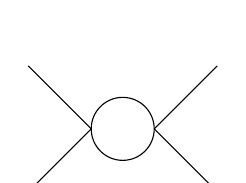
\begin{tikzpicture}[scale=0.8]
    \draw (-1,1)--(0,0);
    \draw (-1,-1)--(0,0);
    \draw (2,1)--(1,0);
    \draw (2,-1)--(1,0);
    \draw(0.5,0) circle (0.5);
  \end{tikzpicture}
  \qquad
  \raisebox{-1.1em}{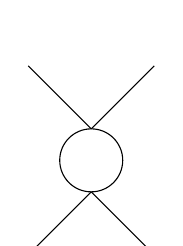
\begin{tikzpicture}[scale=0.8]
    \draw (1,-1)--(0,0);
    \draw (-1,-1)--(0,0);
    \draw (1,2)--(0,1);
    \draw (-1,2)--(0,1);
    \draw(0,0.5) circle (0.5);
  \end{tikzpicture}}
  \qquad
  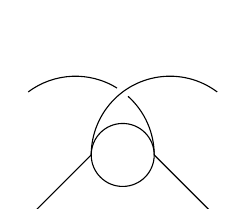
\begin{tikzpicture}[scale=0.8]
    \draw (-1,-1)--(0,0);
    \draw (2,-1)--(1,0);
    \draw (0.5,0) circle (0.5);
    \draw (2,1) arc (53.1301023542:180:1.25);
    \draw (1,0) arc (0:48.1301023542:1.25);
    \draw (0.40999028082,1.06156150515) arc (58.1301023542:126.869897646:1.25);
  \end{tikzpicture}.
  \label{eqn:scalar-second-order-2-2-diagrams}
\end{e}
\jtd{Put in momentum arrows}

These represent the first non-trivial effect of QFT we have seen. Everything we have done so far has confirmed classical expectations, from $M=\lambda$ above to momentum conservation. These diagrams are fundamentally quantum and relativistic phenomena and represent a a true prediction of QFT. Let's compute them using the Feynman rules. Two propagators in each diagram are identical and can be exchanged, so they have symmetry factors of 2. Thus,
\begin{es}
  \mathrm{Left} = -\frac{\lambda^2}{2}\int \ftve{4}{k} \frac{1}{k^2-m^2}\frac{1}{(k - p_1- p_2)^2-m^2}\\
  \mathrm{Center} = -\frac{\lambda^2}{2}\int \ftve{4}{k} \frac{1}{k^2-m^2}\frac{1}{(k - p_1- q_1)^2-m^2}\\
  \mathrm{Right} = -\frac{\lambda^2}{2}\int \ftve{4}{k} \frac{1}{k^2-m^2}\frac{1}{(k - p_1- q_2)^2-m^2}.
  \label{eqn:scalar-second-order-2-2-diagrams-values}
\end{es}
where we have removed the external propagators in the spirit of truncation. It's common to deal with these diagrams by defining \emphi{Mandelstam variables}, which are a reparametrization for any two-to-two-particle interaction:
\begin{e}
  s = (p_1 + p_2)^2\qquad t = (p_1 - q_1)^2 \qquad u = (p_1 - q_2)^2.
  \label{eqn:mandelstam}
\end{e}
There are three variables because momentum conservation makes a fourth one obsolete. They have the interpretation that $s$ is the incoming momentum, equivalently the energy in the center of mass frame, and $t$ and $u$ represent the amount of momentum transfer. Calculation will reveal that each diagram is sensitive only to $s$, $t$, or $u$ respectively, so all three diagrams can be added up as follows:
\begin{e}
  -iM = -i\lambda - \lambda^2\parens{V(s) + V(t) + V(u)} + \mathcal{O}(\lambda^3)
  \label{eqn:2-2-scalar-amplitude}
\end{e}
where
\begin{e}
  V(s) = \frac{1}{2}\int \ftve{4}{k} \frac{1}{k^2-m^2} \frac{1}{(k - p_1 - p_2)^2-m^2}.
  \label{eqn:2-2-scalar-v}
\end{e}
This integral may strike you as a bit peculiar. Let's pretend for a moment that $k^2$ is the Euclidean norm $k_0^2 + \bm k^2$ rather than the Minkowski norm $k_0^2 - \bm k^2$. Then we could switch to spherical coordinates and $d^4 k$ would become $k^3 dk$ times a radial volume element $d\Omega$. For large $k$, this $k^3$ cancels with the integrand, which goes like $k^{-4}$, leading to an overall trend of $\int^\infty dk /k$. This integral is divergent.

The techniques for handling this divergence took a great deal of time to be developed historically. They necessitate a change in thinking which we will discuss in chapter \ref{chap:renormalization}, so we'll postpone this particular integral until then. In three spacetime dimensions (two spatial dimensions), the integral trends to $\int^\infty dk /k^2$ which is a perfectly reasonable number. Figure \ref{fig:2-2-scalar-v-3d} shows the plot of $V(s)$ in three dimensions.\footnote{You might reasonably object to us computing predictions for an unphysical universe, like one with only three spacetime dimensions, in a book about the phenomena of this universe. However, many of the phenomena we'll see are qualitatively similar between dimensions, and the characteristics of dimension four specifically will be covered later.}

\begin{figure}
  \centering
  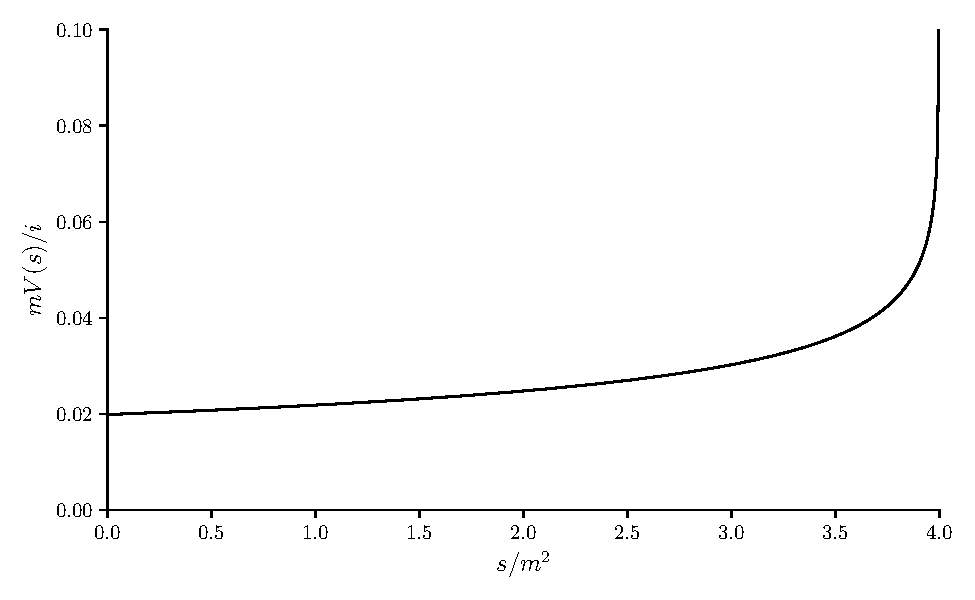
\includegraphics[width=\linewidth]{figs/2-2-scalar-v-3d.pdf}
  \caption{$mV(s)/i$, the unitless second order component of the scattering amplitude. This is computed for two scalar particles in 3 spacetime dimensions of center-of-mass energy $s$.}
  \label{fig:2-2-scalar-v-3d}
\end{figure}

Something immediately apparent about Figure \ref{fig:2-2-scalar-v-3d} is that the values are small. Multiplied by a small number $\lambda^2$ as \ref{eqn:2-2-scalar-amplitude} requires, and this $V(s)$ correction will be tiny except near the maximum value of $s=4m^2$, where the function blows up. This is the hyper-relativistic limit, where the particles are colliding at enormous speeds. In this limit, the quantum corrections introduced by the second-order diagrams can become arbitrarily large. (\ref{eqn:2-2-scalar-v}) is actually analytical computable:
\begin{e}
  V(s) = \frac{i}{16\pi \sqrt{s}}\ln \parens{\frac{m +\sqrt{s/4}}{m -\sqrt{s/4}}}.
\end{e}
We will discuss how to arrive at this value for the integral in chapter \ref{chap:renormalization}.

Taking the limit as $s\rightarrow 4$ reveals that $V(s)$ blows up and scattering becomes extremely intense. This is a QFT correction to the classical expectation that $M = \lambda$; i.e., scattering amplitude is independent of energy.

\subsection{Intuition for Feynman Diagrams}

In the derivation of this chapter, each propagator in a Feynman diagram represents a Wick contraction, but there is an intuitive picture for Feynman diagrams beyond the mathematical structure of Wick's theorem. We already know an external propagator --- a particle that links to an external vertex --- represents a particle entering the scattering experiment. Why not view \textit{every} propagator as a particle? Then the $\phi^4$ term of the Lagrangian, which corresponds to four propagators meeting at a vertex $x$ in a diagram, really does represent an interaction at $x$. A diagram with a loop, such as those in (\ref{eqn:scalar-second-order-2-2-diagrams}), represent two particles colliding, only for the outgoing particles to collide with each other again. If one collision is rare, then this secondary collision should be rarer than one collision only, which explains why these diagrams are small. On the other hand, if a collision is common, we might expect every particle pair to collide not just once or twice but many times, in which case we would have to draw infinitely many diagrams. It is at this point that QFT is no longer perturbative, and alternative methods to Feynman diagrams must be taken to compute scattering amplitudes.

There is a small problem with this picture, however. The two internal propagators in (\ref{eqn:scalar-second-order-2-2-diagrams}) are not real particles in a key sense: they are not on-shell. This can be seen in (\ref{eqn:scalar-second-order-2-2-diagrams-values}): we integrate $k$ over all four-dimensional space without requiring $k^2=m^2$. Instead, we call these internal propagators \emphi{virtual particles}, which interact like normal particles except that they can be off-shell (meaning that $k^2$ needn't equal $m^2$) and are never observed.

These virtual particles could have been predicted even before we saw the QFT principle of least action. One of the major results of special relativity was that mass is a form of energy, and a result of quantum mechanics is that a quantum particle may tunnel through a high-energy barrier in order to reach a low energy final state. Any theory of quantum mechanics and relativity, such as QFT, should combine these two well-understood phenomena. What better way to combine them than to allow particles to ``tunnel'' into an unphysical, perhaps higher-energy state before reaching a final state? The loop propagators represent this higher-energy state, and are unphysical in the same way that the electron should not classically exist in a high-energy barrier in quantum mechanics. Nevertheless, a particle can pass through the high-energy state in order to attain a different final state.

We could even have predicted that virtual particles can be off-shell by another example of hybrid quantum mechanical and relativistic reasoning: the energy-time uncertainty principle predicts that quantum states with a short lifetime have uncertain energies. In a relativistic context, the equivalent statement is that particles with a short lifetime have uncertain mass. Virtual particles are never observed, so they have effectively zero lifetime and infinitely uncertain mass, preventing the enforcement of the on-shell constraint.

We'll often treat any diagram with a loop, such as those of (\ref{eqn:scalar-second-order-2-2-diagrams}), as a ``quantum correction'' --- a small correction quantum mechanics imposes on a classical theory. The loop brings all the quantum effects mentioned in the previous paragraphs into the picture; it is comprised of virtual particles and the $\int d^4 k$ represents the fact that these virtual particles are off-shell. Figure \ref{fig:2-2-scalar-v-3d} for the second-order $\phi\phi \rightarrow \phi\phi$ amplitude was our first example of a quantum corrections, but more will appear such as mass, energy, magnetic and electric dipole moment corrections.

The diagrams without loops, often called \emphi{tree-level diagrams}, generally represent the properties of a classical theory that could be attained by merely minimizing the action via the Euler-Lagrange equations. For example, a tree-level diagram delivered us $M_{\phi\phi\rightarrow \phi\phi} = \lambda$ as classical thinking would suggest.


\section{Complex Scalar Theory}
So far, we've considered only real scalar fields where $\phi^* = \phi$, but one may well ask if complex scalar fields exist. After all, the fermions in Nature can all take on complex values, and the only fundamental scalar particle in Nature (the Higgs) is complex. Fortunately for us, generalizing the above results to a complex field will be mathematically easy. However, it will bring up a critical new physics concept which we will need to understand: the antiparticle.

\subsection{Antiparticles}

The Lagrangian of a complex scalar field is nearly the same as that of a real field. The only differences are coefficients to the term and the presence of complex conjugates:
\begin{e}
  \mathcal{L} = -|\del_\mu \phi|^2 - m^2 |\phi|^2 + \lambda |\phi|^4.
  \label{eqn:complex-scalar-lagrangian}
\end{e}
The reason why the coefficients have changed is so that the counting arguments of table \ref{tab:symmetry-factor} which allow computation of the symmetry factor still apply even though now $\phi^* \neq \phi$.

Immediately, we suspect that $\phi^*$ may be the antiparticle of $\phi$. This is because, as mentioned in chapter \ref{chap:intro}, an antiparticle is the mirror image of a particle under charge reversal. Charge reversal is manifested in complex conjugation for reasons that we will eventually see in chapter \ref{chap:spin-one}, so that charge reversal takes $\phi$ to $\phi^*$. Thus, $\phi^*$ is the antiparticle of $\phi$.

The antiparticle explanation may not be fully satisfying, however, since (\ref{eqn:complex-scalar-lagrangian}) still looks like the Lagrangian of only one particle. Let's therefore break up the $\phi$ field into components. Just as a complex number $z=(a+ib)\sqrt{2}$ can be broken into two real components (the $\sqrt{2}$ is for normalization), the complex field $\phi = (\phi_a + i\phi_b)/\sqrt{2}$ can be broken into real fields $\phi_a$ and $\phi_b$. Plugging these into the Lagrangian, we get
\begin{es}
  \mathcal{L} =& -\frac{1}{2}(\del_\mu \phi_a)^2- \frac{m^2}{2} \phi_a^2 + \frac{\lambda}{4} \phi_a^4\\
  &-\frac{1}{2}(\del_\mu \phi_b)^2 - \frac{m^2}{2} \phi_b^2  + \frac{\lambda}{4} \phi_b^4\\
  &+ \frac{\lambda}{2}\phi_a^2 \phi_b^2.
  \label{eqn:complex-scalar-components}
\end{es}
We can now see that the complex scalar Lagrangian is just two real fields with the same mass $m$, same self-interaction $\lambda$, and an $a-b$ interaction term which is the last line. These properties were required for (\ref{eqn:complex-scalar-lagrangian}) to be written so simply.

The complex scalar Lagrangian (\ref{eqn:complex-scalar-lagrangian}) looks elegant, but when broken into its components it seems oddly contrived. Why should the real and imaginary parts have the same mass and interaction strengths? Why should they interact with each other in the exact way shown by (\ref{eqn:complex-scalar-components})? These constraints are imposed by CPT symmetry. A particle's antiparticle must have the same mass and interactions. Mathematically speaking, they obey a \emphi{symmetry}, in that swapping $\phi_a$ and $\phi_b$ does not change the Lagrangian.

In fact, the symmetry is even deeper than this; any (normalized) linear combination of the two fields is also indistinguishable from $\phi_a$ and $\phi_b$. For example, if we define $\chi_a = (3\phi_a + 4i\phi_b)/5$and $\chi_b = (4\phi_a - 3i\phi_b)/5$, we could rewrite (\ref{eqn:complex-scalar-components}) in terms of $\chi_a$ and $\chi_b$ and we would get the exact same form, just with $\phi$ swapped out for $\chi$. If it weren't for the odd $\frac{\lambda}{2}\phi_a^2\phi_b^2$ interaction term, this would not be true. \jtd{Unitary group too}

This particular symmetry is called SO(2), or \emphi{the Special Orthogonal Group of Order 2}. The name is motivated by the kinds of linear combinations which do not change the Lagrangian; ``special'' indicates that the new linear combinations $\chi$ must remain normalized, ``orthogonal'' indicates that the two fields $\chi_a$ and $\chi_b$ must have the same product as the original $\phi_a\phi_b$, ``group'' indicates that any linear combination that satisfies these two properties is allowed as a symmetry of the Lagrangian, and ``order 2'' means that the linear combination acts on two fields $\phi_a$ and $\phi_b$. This is our first example of a \emphi{continuous symmetry} because the set of available linear combinations is continuous. Nature adores continuous symmetries. The Standard Model which is the best known description of the fundamental particles has three of these symmetries, as will be discussed in the next part of this book.

You might wonder where $\phi$'s antiparticle was for the real scalar field case. For real scalars, the particle is its own antiparticle. This also occurs for some Standard Model particles, such as the photon.

\subsection{Feynman Rules for Complex Scalars}

Now that we have shown that a complex scalar contains an antiparticle, it is time to discuss the Feynman rules of the new theory. Fortunately, we do not have to repeat the many pages of derivations necessary for the real field theory. The Lagrangian is essentially the same, so the Green's function of a complex scalar field is identical to that of a real field. Wick's theorem and its application to the free theory and the interacting theory did not rely on anything other than that the perturbation $\lambda$ is small. Thus, we can skip straight to the rules for how to draw Feynman diagrams.

The new Lagrangian restricts diagrams slightly. The $\phi^4$ term became $\phi^*\phi \phi^*\phi$, meaning that only two antiparticles and two particles can meet at a vertex, not three and one, for instance. We'll have to enforce this in Feynman diagrams with a graphical rule. Suppose we draw an arrow on a propagator, where the arrow points one way for a particle and another way for an antiparticle. Then the $\phi^*\phi \phi^*\phi$ term means every vertex must have two arrows leading in and two leading out. (Since $\phi$ and $\overline \phi$ have opposite charge, you can think of these arrows as charge arrows.) Thus, the Feynman rules are 

\begin{enumerate}
  \item The edge \raisebox{0.2em}{\begin{tikzpicture}[scale=0.8]
    \draw (-0.7,0) -- (0.7,0);
    \draw[-{Latex[length=3mm]}] (-0.3,0) -- (0.15,0);
    \draw (-0,0.1) node[anchor=south]{$k$};
  \end{tikzpicture}} contributes $G(k)$
  \item A vertex \raisebox{-2.3em}{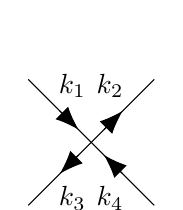
\begin{tikzpicture}[scale=0.8]
    \draw (-1,1) -- (1,-1);
    \draw (-1,-1) -- (1,1);
    \draw[-{Latex[length=3mm]}] (-0.5,0.5) -- (-0.2,0.2);
    \draw (-0.3,0.55) node[anchor=south]{$k_1$};
    \draw[{Latex[length=3mm]}-] (0.5,0.5) -- (0.2,0.2);
    \draw (0.3,0.55) node[anchor=south]{$k_2$};
    \draw[{Latex[length=3mm]}-] (-0.5,-0.5) -- (-0.2,-0.2);
    \draw (-0.3,-0.55) node[anchor=north]{$k_3$};
    \draw[-{Latex[length=3mm]}] (0.5,-0.5) -- (0.2,-0.2);
    \draw (0.3,-0.55) node[anchor=north]{$k_4$};
  \end{tikzpicture}} contributes $-i\lambda \delta(k_1 - k_2 - k_3 + k_4)$
  \item Every internal propagator $k$ is integrated over $\int \ftve{4}{k}$
  \item Diagrams with exchangeable vertices or reversible edges contribute a symmetry factor $S_f$.\footnote{You might recall that the definition of $S_f$ derived from a counting problem for how much each diagram should be weighted by, and that problem depended on $\phi$ being real. The coefficients of the new Lagrangian (\ref{eqn:complex-scalar-lagrangian}) have been carefully chosen so that the definition of the symmetry factor is the same, so we don't have to worry about redoing that argument.}
\end{enumerate}
We stopped drawing the momentum arrows in the diagrams to reverse clutter. There's no harm in just defining momentum to point in the same direction as the charge arrows.

As an example, here are the diagrams of (\ref{eqn:scalar-second-order-2-2-diagrams}) for a complex scalar field, representing $\phi \overline\phi \rightarrow \phi \overline\phi$ scattering:

\begin{e}
  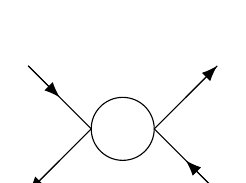
\begin{tikzpicture}[scale=0.8]
    \draw (-1,1)--(0,0);
    \draw[-{Latex[length=2mm]}](-1,1)--(-0.5,0.5);
    \draw (-1,-1)--(0,0);
    \draw[{Latex[length=2mm]}-](-1,-1)--(-0.5,-0.5);
    \draw (2,1)--(1,0);
    \draw[{Latex[length=2mm]}-](2,1)--(1.5,0.5);
    \draw (2,-1)--(1,0);
    \draw[-{Latex[length=2mm]}](2,-1)--(1.5,-0.5);
    \draw(0.5,0) circle (0.5);
  \end{tikzpicture}
  \qquad
  \raisebox{-1.1em}{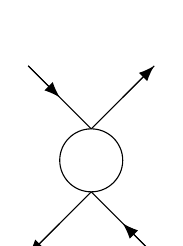
\begin{tikzpicture}[scale=0.8]
    \draw (1,-1)--(0,0);
    \draw[-{Latex[length=2mm]}](1,-1)--(0.5,-0.5);
    \draw (-1,-1)--(0,0);
    \draw[{Latex[length=2mm]}-](-1,-1)--(-0.5,-0.5);
    \draw (1,2)--(0,1);
    \draw[{Latex[length=2mm]}-](1,2)--(0.5,1.5);
    \draw (-1,2)--(0,1);
    \draw[-{Latex[length=2mm]}](-1,2)--(-0.5,1.5);
    \draw(0,0.5) circle (0.5);
  \end{tikzpicture}}
  \qquad
  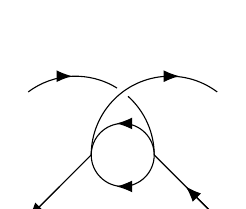
\begin{tikzpicture}[scale=0.8]
    \draw (-1,-1)--(0,0);
    \draw[{Latex[length=2mm]}-](-1,-1)--(-0.5,-0.5);
    \draw (2,-1)--(1,0);
    \draw[-{Latex[length=2mm]}](2,-1)--(1.5,-0.5);
    \draw (0.5,0) circle (0.5);
    \draw (2,1) arc (53.1301023542:180:1.25);
    \draw[-{Latex[length=2mm]}](-0.4,1.25)--(-0.3,1.25);
    \draw[{Latex[length=2mm]}-](1.4,1.25)--(1.3,1.25);
    \draw (1,0) arc (0:48.1301023542:1.25);
    \draw (0.40999028082,1.06156150515) arc (58.1301023542:126.869897646:1.25);
    \draw[{Latex[length=2mm]}-](0.4,-0.5)--(0.5,-0.5);
    \draw[{Latex[length=2mm]}-](0.4,0.5)--(0.5,0.5);
  \end{tikzpicture}.
\end{e}

There are similar diagrams for $\phi\phi \rightarrow \phi \phi$ scattering:

\begin{e}
  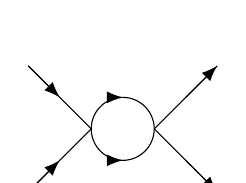
\begin{tikzpicture}[scale=0.8]
    \draw (-1,1)--(0,0);
    \draw[-{Latex[length=2mm]}](-1,1)--(-0.5,0.5);
    \draw (-1,-1)--(0,0);
    \draw[-{Latex[length=2mm]}](-1,-1)--(-0.5,-0.5);
    \draw (2,1)--(1,0);
    \draw[{Latex[length=2mm]}-](2,1)--(1.5,0.5);
    \draw (2,-1)--(1,0);
    \draw[{Latex[length=2mm]}-](2,-1)--(1.5,-0.5);
    \draw(0.5,0) circle (0.5);
    \draw[-{Latex[length=2mm]}](0.4,-0.5)--(0.5,-0.5);
    \draw[-{Latex[length=2mm]}](0.4,0.5)--(0.5,0.5);
  \end{tikzpicture}
  \qquad
  \raisebox{-1.1em}{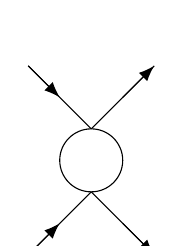
\begin{tikzpicture}[scale=0.8]
    \draw (1,-1)--(0,0);
    \draw[{Latex[length=2mm]}-](1,-1)--(0.5,-0.5);
    \draw (-1,-1)--(0,0);
    \draw[-{Latex[length=2mm]}](-1,-1)--(-0.5,-0.5);
    \draw (1,2)--(0,1);
    \draw[{Latex[length=2mm]}-](1,2)--(0.5,1.5);
    \draw (-1,2)--(0,1);
    \draw[-{Latex[length=2mm]}](-1,2)--(-0.5,1.5);
    \draw(0,0.5) circle (0.5);
  \end{tikzpicture}}
  \qquad
  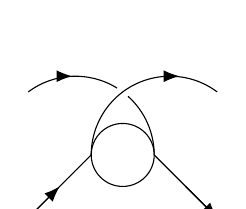
\begin{tikzpicture}[scale=0.8]
    \draw (-1,-1)--(0,0);
    \draw[-{Latex[length=2mm]}](-1,-1)--(-0.5,-0.5);
    \draw (2,-1)--(1,0);
    \draw[{Latex[length=2mm]}-](2,-1)--(1.5,-0.5);
    \draw (0.5,0) circle (0.5);
    \draw (2,1) arc (53.1301023542:180:1.25);
    \draw[-{Latex[length=2mm]}](-0.4,1.25)--(-0.3,1.25);
    \draw[{Latex[length=2mm]}-](1.4,1.25)--(1.3,1.25);
    \draw (1,0) arc (0:48.1301023542:1.25);
    \draw (0.40999028082,1.06156150515) arc (58.1301023542:126.869897646:1.25);
  \end{tikzpicture}.
\end{e}
When a loop is drawn without charge arrows, the charge arrows can go either way so long as they are antiparallel. This does \textit{not} count as a reversible edge in the symmetry factor sense; a symmetry factor represents that we have overcounted a diagram, whereas if a loop can run either of two directions we are undercounting the diagrams. Thus, we should double each diagram where the loop can run either day, not half it.

Thus, a difference between complex scalar scattering and real scalar scattering is that the quantum corrections to complex scattering is more intense. Contributions from both particles and antiparticles can occur, increasing the total interaction strength. The exception is in some channels which forbid particle-antiparticle interactions. For example, for $\phi \phi \rightarrow \phi\phi$, the $s$ channel is not amplified because only $\phi$ particles may mediate that interaction. In $\phi \overline\phi \rightarrow \phi\overline\phi$, the $u$ channel is not amplified.

One of the most famous properties of matter and antimatter is that they explode on contact with each other. Electrons and positrons annihilate to two or three photons, as do neutral pions. Charged pions decay to muons and neutrinos, et cetera. In the next section,  we'll introduce a real scalar field as a photon-like particle and compute amplitudes for a complex scalar field to decay in this theory.

\section{Scalar Decay}
Let's create a theory with two particles: a complex scalar $\phi$ and a real scalar $\chi$ and an interaction between them of $\phi \phi^* \chi$. This corresponds to a Lagrangian of
\begin{e}
  \mathcal{L} = -|\del_\mu \phi|^2 - m_\phi|\phi|^2 - \frac{1}{2}(\del_\mu \chi)^2 - \frac{1}{2}m_\chi\chi^2 - g \phi\phi^* \chi.
\end{e}
In order to draw Feynman diagrams for a system with two particles, we need two types of lines --- a dashed line for $\chi$ and a solid line for $\phi$. The Feynman rules are as you might guess; the $\phi$ and $\chi$ propagators are still $G(k)$, momentum conservation is still applied at every vertex, and internal propagators are still integrated over. The only difference comes from the new interaction terms, which allows vertices connecting two $\phi$ particles to one $\chi$ particle
\begin{center}
  \feynmandiagram [horizontal=b to a, scale=0.8] {
    i1 -- [fermion] b -- [fermion] i2,
    a -- [scalar] b,
  };
\end{center}
which contributes an amplitude of $-ig$. Note that there is no charge arrow on the dashed $\chi$ line because $\chi$ is real and therefore uncharged.

Many interesting phenomena can be studied in this theory, but in this section we will only focus on one: the decay of $\chi$ into two $\phi$ particles. Due to energy conservation, this decay can only occur if $m_\chi > 2m_\phi$, so we assume this inequality.

The leading order interaction for decay is just the above Feynman diagram with some added labels
\begin{center}
  \feynmandiagram [vertical=b to a, scale=0.8] {
    i1 -- [fermion, momentum=$q$] b -- [fermion, momentum=$q$] i2,
    a -- [scalar, momentum=$0$] b,
  };
\end{center}
We've also rotated the diagram because, when drawing diagrams for scattering experiments, it is traditional to put the initial state at the bottom and the final state at the top so that time flows upwards as in embedding diagrams in relativity. We assumed that the $\chi$ particle is at rest, which we can always undo by boosting into a different reference frame if needed. The only truncated next order diagram is
\begin{center}
  \feynmandiagram [vertical=b to a, scale=0.8] {
    i1 -- [fermion] p1 -- [fermion, momentum=$q-k$] b -- [fermion, momentum=$q-k$] p2 -- [fermion] i2,
    a -- [scalar] b,
    p1 -- [scalar, momentum'=$k$] p2,
  };
\end{center}
Together, these diagrams produce a decay amplitude of 
\begin{e}
  iM = -ig + (-ig)^3\int \ftve{4}{k} \frac{1}{k^2-m_\chi^2}\frac{1}{[(q-k)^2-m_\phi^2]^2}
\end{e}
which yields a decay rate given by (\ref{eqn:total-decay-rate}). For the rest of this discussion, we'll neglect the second order term and just use $M=-g$.

Energy conservation gives $2q^0 = m_\chi$ and the on-shell constraint dictates that $(q^0)^2 - \bm q^2 = m_\phi^2$, so the momentum of the outgoing particles is $\bm q^2 = m_\phi^2 - m_\chi^2 / 4$. Thus, the three-dimensional integral over outgoing momenta is actually a two-dimensional integral on a sphere, and the spherical symmetry of this decay problem implies that the value is $4\pi$ times the integrand. Thus,
\begin{e}
  \Gamma = \frac{|M_{p\rightarrow q}|^2}{(2\pi)^5 m_\chi^3}\parens{m_\phi^2 - \frac{m_\chi^2}{4}}
\end{e}
It's more interesting to compute the unitless constant $\Gamma m_\chi^2$ --- physically, the probability to decay within one Compton wavelength of the particle, as a function of the ratio of $\mu = 2m_\phi / m_\chi < 1$. This is
\begin{e}
  m_\chi \Gamma = \frac{1-\mu^2}{4(2\pi)^5}g^2
\end{e}

One can see that as the decay products get lighter and $\mu$ gets smaller, the lifetime of $\chi$ becomes shorter. This is intuitively what we expect of our first every decay width calculation. Decay is the relativistic version of quantum tunneling into a new state, and quantum tunneling is generally more likely to happen if the potential energy of the end state is lower. Here, the mass energy of the end state is proportional to $\mu$, so we expect the lifetime to decrease with $\mu$. 

Another intuitive fact is that, for $\mu = 0$, $\Gamma$ reaches a finite value. This is something we should have expected because many particles in Nature, such as the pion, decay into massless photons. Yet the neutral pion has a relatively long lifetime of seconds, corresponding to a travel distance of 25 nanometers when moving at the speed of light (many particles live even shorter lives). Ignoring the fact that photons are not complex scalar particles, it would be concerning if our current calculations predicted zero lifetime for such decays.

If $m_\chi < m_\phi$, this decay is energetically forbidden, and completely new physics arises from the same Lagrangian which is discussed in the next section.

\section{Coulomb Potential for Scalars}
\label{sec:scalar-coulomb}
One of the foundational assumptions of QFT was that the theory is local, meaning that every particle is influenced only by its immediate environment. This might seem obviously incorrect at first because of long-range forces like Coulomb's law, which allow distant objects to affect one another. But in electromagnetism we explained these forces via a field which propagates information between objects by the means of waves, and in QFT we graduate those waves to particles. In this section we use the same Lagrangian as in the previous to demonstrate a long-range force carrier.

As an experiment to look for forces, we could scatter a complex scalar $\phi$ particle off of an equally charged $\phi$ particle and measure the cross section. The light, real scalar $\chi$ will carry the force between the two particles. The leading order diagram for this interaction is
\begin{center}
  \feynmandiagram [horizontal=b to a] {
    i1 -- [fermion, momentum'=$p_1$] b -- [fermion, momentum'=$q_1$] i2,
    j1 -- [fermion, momentum=$p_2$] a -- [fermion, momentum=$q_2$] j2,
    b -- [scalar, momentum=$p_1 - q_1$] a,
  };
\end{center}
If the outgoing particles were distinguishable then there would be a second diagram wherein the particles are swapped, but in this case the outgoing particles are equally charged and are indistinguishable. Setting $m_\chi=0$, the scattering amplitude is
\begin{e}
  iM = \frac{-ig^2}{(p_1 - q_1)^2}
\end{e}
which is just a constant times the Green's function for the one internal propagator.

We can use this scattering amplitude to compute the equivalent of the potential between the particles if we make a few approximations. Firstly, we'll work in the non-relativistic limit, where the energies of all particles is approximately their masses, in which case $p_1 - q_1$ has zero temporal component. The second approximation is to compare this amplitude with that predicted by non-relativistic quantum mechanics under the Born approximation, as discussed in appendix \ref{app:quantum}. That amplitude is $M(\bm p_1 - \bm q_1) = -V(\bm p_1 - \bm q_1)$ where $V$ is the Fourier transform of the potential between particles. Plugging in our amplitude calculation, we have
\begin{e}
  V(\bm x) = -g^2\int \ftve{3}{\bm \ell}\frac{e^{i\bm \ell \cdot \bm x}}{\bm \ell^2}
\end{e}
where $\bm \ell = \bm p_1 - \bm p_2$. By inspection, the integral cannot depend on the orientation of $\bm x$, so we write $\bm x = r \hat{\bm z}$ and switch to spherical coordinates:
\begin{es}
  V(r) &= -\frac{g^2}{4\pi^2} \int_{-1}^1 d\cos\theta \, \int_0^\infty d\ell \, e^{i\ell r \cos \theta}\\
  &= -\frac{g^2}{8\pi^2}\int_{-1}^1 d\cos\theta \, \int_{-\infty}^\infty d\ell \, e^{i\ell r \cos \theta}\\
  &= -\frac{g^2}{4\pi}\int_{-1}^1 d\cos\theta \, \delta(r \cos \theta)\\
  &= -\frac{g^2}{4\pi r}\\
\end{es}
The second line came about by recognizing that the real part of the integrand was symmetric under $\ell \rightarrow -\ell$, so we could extend the $\ell$ integral. The third line applied the theorem connecting the integral of an oscillating exponent to the delta function. The last line came from the fact that $\delta(f(x)) = \delta(x)/f'(x)$.

If we interpret the $g$ as the ``charge'' of the scalar particle, then the result is the Coulomb potential! In case the QFT principle of least action were still in doubt, this is an excellent sign that the theory is pointing us in the right direction. The only strangeness is that the sign is wrong; these like-charged particles are attracted to each other whereas in electromagnetism they would be repelled. This is a result of our choice to use scalar particles. In the next two chapters we will introduce new particles which are capable of flipping this sign to become more electromagnetism-like.

Another motivation for us to pursue more particles to describe electromagnetism is that this theory contains no magnetic field. There aren't enough degrees of freedom in the particles provided to store the direction of an additional field, and adding new ``magnetic field particles'' would not be able to interact so as to guarantee Maxwell's equations. We will need a particle capable of encoding the direction of the magnetic field within its quantum state.


\section{Massless Scalars are Rare}
\label{sec:scalar-mass}
One final problem with the Coulomb-like potential derived in the previous section is that massless scalars are unlikely to occur. To see why, recall from chapter \ref{chap:spectrum} that the 2PCF of a particle contains a pole at the particle's mass. We can compute the 2PCF of the $\chi$ particle using the Lagrangian above to see where its pole is. The first two orders of Feynman diagrams are 
\begin{center}
  \feynmandiagram [horizontal=b to a] {
    b -- [scalar, momentum'=$p$] a
  };
  \qquad
  \feynmandiagram [layered layout, horizontal=b to c] {
    a -- [scalar, momentum=\(p\)] b
    -- [fermion, half left, looseness=1.5, momentum=\(k\)] c
    -- [fermion, half left, looseness=1.5, momentum=\(k-p\)] b,
    c -- [scalar, momentum=\(p\)] d,
  };
\end{center}
which correspond to a 2PCF of
\begin{e}
  \int d(\mu^2)\, \rho(\mu^2) \frac{1}{p^2-\mu^2} =  \frac{1}{p^2}\brackets{1 + \frac{\Sigma}{p^2}}.
\end{e}
where we used the definition of $\rho$ from (\ref{eqn:spectral-density}), and
\begin{e}
  \Sigma = (-ig)^2\int \ftve{4}{k}\frac{1}{k^2 - m_\phi^2}\frac{1}{(p-k)^2 - m_\phi^2}.
\end{e}
Note that the external legs are included because we are computing a 2PCF, not a scattering amplitude.

We could have continued adding loops, leading to diagrams such as 
\begin{center}
  \feynmandiagram [layered layout, horizontal=b to c, scale=0.8] {
    a -- [scalar] b
    -- [fermion, half left, looseness=1.5] c
    -- [fermion, half left, looseness=1.5] b,
    c -- [scalar] d
    -- [fermion, half left, looseness=1.5] e
    -- [fermion, half left, looseness=1.5] d,
    e -- [scalar] f
    -- [fermion, half left, looseness=1.5] g
    -- [fermion, half left, looseness=1.5] f,
    g -- [scalar] h,
  };
  $\cdots$
\end{center}
Adding together all the contributions from all numbers of loops gives
\begin{es}
  \int d(\mu^2)\, \rho(\mu^2) \frac{1}{p^2-\mu^2} &=  \frac{1}{p^2}\brackets{1 + \frac{\Sigma}{p^2} + \frac{\Sigma^2}{p^4} + \cdots}\\ = \frac{1}{p^2}\frac{1}{1 - \Sigma/p^2} &= \frac{1}{p^2 - \Sigma}.
\end{es}
Surprisingly, the loops move the spike in the spectral density $\rho(\mu^2)$ from zero to $\mu^2 = \Sigma$, in violation of our expectation that the mass of the $\chi$ particle should be $m_\chi$, which is zero\footnote{We have implicitly assumed that $\Sigma \neq 0$. This assumption is correct, but we will not have the mathematical tools to evaluate $\Sigma$ until chapter \ref{chap:renormalization}.}.

This fact leaves an interesting question. If the spike in the spectral density $\rho$ need not equal the particle mass in the Lagrangian, which should we interpret as mass? It is tempting to continue to quote the $m_\chi$ in the Lagrangian as the mass of the particle because it is an intuitive quantity, but this number is not actually observable while the spike in the spectral density is. As we mentioned earlier in this chapter, the spike also plays the key role of ensuring that any particle's momentum always obeys the relativistic $p^2 = m^2$ constraint. The square of the 2PCF gives the probability of a state being observed, so if the 2PCF blows up for $p^2$ equal to a certain amount it makes sense to define that amount as the mass.

This realization --- one might say betrayal --- that the Lagrangian mass is not the true mass of the particle has a physical explanation, which also explains why we only noticed the difference between the Lagrangian mass and the spectral mass (the true mass) when we looked at a loop diagram. When a $\chi$ particle is moving through space, this loop represents the creation of virtual $\phi$-anti$\phi$ pairs that immediately annihilate. This happens at all times at all points in space and is an inevitable prediction of a quantum theory that allows tunneling. We never observe these virtual particles, but their presence temporarily increase the rest energy of the $\chi$ particle and is responsible for the shift in the spike of $\rho(\mu^2)$. Thus, when we observe the $\chi$ particle we also observe the shadow of the $\phi$ particles it is coupled to.

One might be suspicious of this rather hand-wavy argument, but some experiments confirm that this particle-antiparticle creation and annihilation is exactly what is happening. Specifically, when measurements are made in an extremely small volume or extremely close to another particle, these particle-antiparticle pairs have less room to form and are suppressed. The Lagrangian mass being exposed a little, and the observed properties of particles start to change. For example, when an electron is put very close to a proton, the charge of both appears to increase a little and this results in a small shift in the energy of the $s$ orbitals of hydrogen known as the Lamb shift. Another example is that when you put two plates very close to each other, the particle-antiparticle pairs that occur naturally in a vacuum are suppressed between them, and the pressure of these pairs outside the plates forces them together in a phenomenon known as the Casimir effect. The mathematical description for these effects will be given in chapter \ref{chap:renormalization}.

This mass shift is why the title of this section is that massless scalars are rare. In order for $\chi$ to be observed as massless --- that is, the spike of its spectrum is at zero --- its $m_\chi$ value in the Lagrangian must be ``fine tuned'' such that the loop diagram and all higher order loop diagrams cancel exactly with $m_\chi$ and move the spike of the spectrum to zero. Historically, a theory that requires parameters to be finely tuned to reproduce observations has been ill-trusted because it suggests the existence of some unexplained structure to the universe. Fortunately, we do not observe any massless scalars in Nature, so there is no fine tuning problem. The only massless particles are vector bosons, which we will see in chapter \ref{chap:spin-one} cannot be made massive by loop diagrams.




\begin{problem}[Wick's Theorem]
  In section \ref{sec:wicks-theorem}, we explained Wick's theorem, which is that 
  $\frac{d^nZ}{d J_{j_1}\dots dJ_{j_n}}$ is equal the sum of $M^{-1}_{ab}$, where $a, b$ are pairs of $j_1,\dots j_n$. This was shown for $n=2$ in (\ref{eqn:2pcf-wick}). Prove via induction that this fact holds for $n>2$.
\end{problem}

\begin{problem}[Momentum Conservation]
  In this question, we'll determine why momentum conservation came so naturally out of the QFT principle of least action.
  \begin{enumerate}
    \item Show that all Feynman diagrams, of any order and with any number of external vertices, conserve momentum in that if the external momenta do not sum to zero, then the $n$PCF is zero.
    \item \jtd{Connect this to the real-ness of the Lagrangian via Fourier transform logic}
    \item Show that the operator $e^{iH}$ is unitary if and only if $H$ is Hermitian. Since the integrand of the QFT principle of least action is $e^{i\mathcal{L}}$, where $\mathcal{L}$ is real, the conservation of momentum structure we got is just the requirement that $e^{i\mathcal{L}}$ be unitary. Unitarity is a property of non-relativistic quantum mechanics that was necessary for the probability to detect a particle not to change over time. The QFT principle of least action is written to preserve unitarity in the sense of momentum conservation, even though this theory can create and destroy particles.
  \end{enumerate}
\end{problem}

\begin{problem}[Symmetry Factors]
  \jtd{Evaluate some diagrams and find some symmetry factors}
\end{problem}

\begin{problem}[New Lagrangians]
  Suppose we designed a new scalar theory in which $\phi$ were real. This allows us to write a cubic term in the Lagrangian instead of a quartic term:
  $$\mathcal{L} = \frac{1}{2}(\del_\mu \phi)^2 - m^2 \phi^2 + \frac{g}{3!}\phi^3.$$
  Write out the Feynman rules for this theory. What would be the Feynman rules of the Lagrangian
  $$\mathcal{L} = \frac{1}{2}(\del_\mu \phi)^2 - m^2 \phi^2 + \frac{g'}{4}\phi^2(\del_\mu \phi)^2?$$
  Hint: this question requires very little math.
\end{problem}

\begin{problem}[Coulomb potentials]
  Using the same Lagrangian as section \ref{sec:scalar-coulomb}, determine whether oppositely charged $\phi$ particles repel or attract.
\end{problem}

\begin{problem}[Coulomb potentials]
  Section \ref{sec:scalar-coulomb} showed that scalar particles reproduce Coulomb's force.
  \begin{enumerate}
    \item Convince yourself that the reason why Coulomb's force was reproduced was that the diagram we were using evaluated to a single particle propagator, and that the form of this propagator came from the kinetic term in the Lagrangian
    \item The Coulomb potential is sometimes justified via Gauss's law, that $\nabla^2 V(x) \propto \rho(x)$. Like the Lagrangian, this is a local equation. Argue that it is unsurprising that the Lagrangian kinetic term and Gauss's law should have both led to the same conclusion.
  \end{enumerate}
\end{problem}
\chapter{Spin One Half}
\label{chap:spin-one-half}

\noindent This chapter deals with extending QFT to cover particles with spin, also known as \emphi{fermions}. Spin is covered in non-relativistic quantum mechanics, though its properties seem sometimes mysterious and arbitrary. In particular, the fact that fermions obey the Pauli exclusion principle and bosons do not cannot be explained in non-relativistic quantum mechanics. This explanation is provided by relativity in QFT in the form of the spin-statistics theorem, which we explain in this chapter. Before arriving at this key result, however, we discuss spin in a generalized sense (section \ref{sec:non-rel-spin}) and show that when relativity is taken into account, spin implies the existence of antiparticles (section \ref{sec:clifford}).

Let's start with a simple definition: spin is the intrinsic angular momentum of a particle. In order to store a particle's spin state in QFT we'll need to graduate our scalar field particle operator $\hat \phi$ to a vector of operators $\hat \psi = (\hat \psi_0, \hat \psi_1,\dots)^T$. This vector is called a \emphi{spinor}.

The next section uses the definition of spin as intrinsic angular momentum to dictate how many entries the spinor must have and what operators can act on it. Our discussion will start with the non-relativistic case, where we do not consider boosts, and then we will add boosts to see how they change the discussion. Following this, we'll describe how to similarly graduate the $\psi$ in the path integral of the QFT principle of least action to a spinor. With this complete, we will repeat the analysis of the previous chapter and derive Feynman rules for fermions. Finally, we will use these new fermions to understand electrons, the Coulomb potential, and atomic nuclei.

\section{Spinors and Spin Operators}
\label{sec:non-rel-spin}

Spin is a quantum state, and in any quantum theory, a quantum state is acted on by operators. It will require the description of new mathematical tools which come from the field of group theory, but by the end we will have a complete description of any particle with spin.

To measure the spin of a spinor $\psi$, we act on $\psi$ with a vector of operators $\bm S$. In order to be interpreted as an angular momentum vector, $\bm S$ must satisfy the defining feature of angular momentum: 

\begin{center}
  \textit{Angular momentum generates rotations.}
\end{center}

The notion of a \emphi{generator} is our first group theoretic term and we will define it in the following paragraph. But first, this definition of angular momentum is different from the classical definition of $\bm L = \bm r \times \bm p$. It is nevertheless a correct definition due to Noether's theorem, which states that an operator's generator is conserved if that operator is a symmetry of the Hamiltonian (appendix \ref{app:noether}). Rotations are a symmetry of spacetime, meaning that if angular momentum generates rotations then angular momentum is conserved. The cross product definition of the angular momentum will return later in this section.

\subsection{Generators}

Now to define what a generator is. Consider a rotation operation $R$ which acts on a three-component vector. We know that $R$ can be written as products of the three-dimensional rotation matrices:
\begin{ec}
  R_x(\theta) = \parens{\begin{matrix}1 & 0 & 0 \\ 0 & \cos\theta & -\sin\theta \\ 0 & \sin\theta & \cos \theta\end{matrix}}\qquad 
  R_y(\theta) = \parens{\begin{matrix}\cos\theta&0&\sin\theta \\ 0&1&0 \\ -\sin\theta & 0 & \cos \theta\end{matrix}}\\
  R_z(\theta) = \parens{\begin{matrix}\cos\theta & -\sin\theta & 0 \\ \sin\theta & \cos \theta & 0 \\ 0&0&1\end{matrix}}.
  \label{eqn:rotation-matrices}
\end{ec}
This fact shows that there are many possible rotation matrices, but that they can each be traced down to the three matrices above. In fact, the above rotation matrices can be simplified even more by writing $R_j(\theta) = e^{i\theta S_j}$, where 
\begin{ec}
  S_x = \frac{i}{2}\parens{\begin{matrix}0 & 0 & 0 \\ 0 & 0 & -1 \\ 0 & 1 & 0\end{matrix}}\qquad 
  S_y = \frac{i}{2}\parens{\begin{matrix}0&0&1 \\ 0&0&0 \\ -1 & 0 & 0\end{matrix}}\\
  S_z = \frac{i}{2}\parens{\begin{matrix}0 & -1 & 0 \\ 1 & 0 & 0 \\ 0&0&0\end{matrix}}.
  \label{eqn:rotation-generators}
\end{ec}
You can check for yourself that exponentiating these matrices gives back the rotation matrices. An arbitrary rotation can therefore be written as 
\begin{e}
  R = e^{i\bm \theta \cdot \bm S}
  \label{eqn:rotation-generation}
\end{e}
where we have arranged $S_x$, $S_y$, and $S_z$ into a vector called $\bm S$. The three components of the vector $\bm \theta$ are called Euler angles and they parameterize the rotation matrix $R$.

In mathematical language, we say that $\bm S$ \emph{generates} the rotations because all rotations can be achieved by plugging different values of $\bm \theta$ into (\ref{eqn:rotation-generation}). The fact that angular momentum is generated by rotation could mean that we should just take $\bm S$ as the spin operator $\bm S$, and write the spinor as a three dimensional vector which $\bm S$ acts on.

\subsection{Angular Momentum Algebra}

This procedure does not work in practice because there are other ways to generate rotations. One can rotate a complex vector for instance, in which case we need a new set of $\bm S$ matrices which are themselves complex. There is an even finer point which must be made: it is necessary that $\bm S$ generate a three-dimensional rotation since spacetime is invariant under three-dimensional rotations. However, the matrix $R$ need not act on a three-dimensional vector. $R$ could act on a five-dimensional vector, for example, and rotate only in a three-dimensional subspace. In this case $\bm S$ would still contain three generators, but each generator would be a $5\times 5$ matrix rather than $3\times 3$.

We therefore need to write a more general definition of rotations than just the rotation matrices (\ref{eqn:rotation-matrices}). One property rotations must have is that they must preserve the length of vectors. That is, $R$ must be unitary. Problem \jtd{cite} asks the reader to show that for $\bm e^{iM}$ to be unitary, $M$ must be hermitian and determinant 1. Thus, the entries of $\bm S$ are hermitian.

The other required property of rotations comes from the way in which they anticommute. Consider rotating a vector aligned with the $z$-axis. If we rotate in the $x$ direction by a small angle $\delta$ first and then $y$ by the same $delta$, we get a different vector than rotating in the $y$ direction first then $y$. This is because the rotation matrices anticommute. Using (\ref{eqn:rotation-matrices}) or drawing pictures that the two rotations differ by a rotation about the $z$ axis by angle $\delta^2$. We can turn this fact into a constraint on $\bm S$ by using (\ref{eqn:rotation-generation}) to define the $x$, $y$, and $z$ rotations. They show that $S_xS_y - S_yS_x = i S_z$.

In principle, we could have aligned our initial vector along any axis $z$, so that the more general version of this constraint is
\begin{e}
  \brackets{S_i, S_j} = i\epsilon_{ijk}S_k
  \label{eqn:angular-momentum-algebra}
\end{e}
where $\epsilon_{ijk}$ is the Levi-Civita symbol. Any set of hermitian, determinant one matrices $\bm S = (S_x, S_y, S_z)$ which satisfies this equation is a valid angular momentum operator. We usually refer to (\ref{eqn:angular-momentum-algebra}) as an \emphi{angular momentum algebra}, and matrices that satisfy it are \emphi{representations} of the angular momentum algebra

\subsection{Using Lie groups to find representations of the angular momentum algebras}
The task of finding matrices $\bm S$ which satisfy (\ref{eqn:angular-momentum-algebra}) (or in mathematical language, finding representations of the angular momentum algebra) has fortunately been solved using group theory. A Lie group is a closed, continuous set of operators, where closed signifies that two operators in the group $U$ and $V$ multiply to produce another operator $W$ which is also in the group. We have unknowingly been working with the group of rotations in three dimensions, which is called the ``special orthogonal group of order three,'' or SO(3). ``Special'' means that the group operators do not change the length of vectors, ``orthogonal'' means that the group operators are real and unitary, and the three indicates that the rotation occurs in three dimensions.

A Lie group satisfies the general result that any group element $G$ can be written as 
\begin{e}
  G = e^{i\bm \theta \cdot \bm S}
  \label{eqn:lie-algebra-generator}
\end{e}
where $\bm S$ are a special set of matrices known as the generators of the Lie group. We used this property in (\ref{eqn:rotation-generation}), but we did not know that it was valid for any Lie groups. The matrices $\bm S$ must satisfy special relations to each other which are dependent on the Lie group the generate; these relations are called a Lie algebra. An example is the angular momentum algebra we discussed above, which we now know as the Lie algebra of SO(3). Mathematicians sometimes label this algebra as $\mathfrak{so}(3)$ but physicists usually use SO(3) to refer to the algebra in addition to the group. We will therefore use the $\mathfrak{so}(3)$ notation in this section only.

Once we specify the dimensions of the spinor which the group elements act on --- say the spinor has dimension $n$, then we can write group elements as $n\times n$ matrices. This is called a representation. Our three-dimensional rotation matrices (\ref{eqn:rotation-matrices}) were a representation of SO(3), and our three-dimensional angular momentum operators (\ref{eqn:rotation-generators}) were representations of its Lie algebra. Matrix exponentiating the generators as in (\ref{eqn:lie-algebra-generator}) can be used to produce the representation of the group if a representation of the Lie Algebra is known.

\subsection{Physical consequences of the group theory explanation for spin}

This new formalism connects directly to the definition used at the beginning of this section --- ``Angular momentum generates rotations.'' The connection is that ``rotations'' refers to the Lie group SO(3), which has the Lie algebra given in (\ref{eqn:angular-momentum-algebra}). The angular momentum operators we're looking for are the rotation generators, which are representations of this Lie algebra.

One reason why this group theory framework is necessary is because (\ref{eqn:angular-momentum-algebra}) is not just the Lie algebra of SO(3). It is also the Lie algebra of SU(2), which is the set of unitary matrices which rotate a two-dimensional complex vector, rather than a three-dimensional real vector. Valid angular momentum operators could therefore be generators of SO(3) or SU(2).

Another use of group theory is the mathematical result that all the faithful\footnote{A faithful representation is one where every group element corresponds to exactly one matrix. For odd dimensions, SU(2) is not faithful because every group element corresponds to two matrices which can be generated using $e^{i\bm \theta \cdot \bm S}$.} representations of SO(3) have odd dimensions, and all the representations of SU(2) have odd\footnote{Except, that is, for the trivial representation, where all the generators are the $1\times 1$ matrix with zero as the only element.} dimensions. Therefore, the spinor which the spin operators act on can have any number of dimensions $n$. If $n$ is even, then one uses representations of $\mathfrak{su}(2)$ as spin operators. If $n$ is odd, one uses representations of $\mathfrak{so}(3)$.

This fact that the parity of $n$ changes what group the spin operators come from has several fascinating properties. Firstly, it means that the SU(2) spins may have different properties than the SO(3) spins. This is manifested in the spin-statistics theorem, which is described in the next section. It also means that since SU(2) acts on complex vectors and SO(3) acts on real vectors. This is crucial because, as noted in the previous chapter, complex particles have an electric charge. Thus, all SU(2) particles are automatically charged. SO(3) particles can be neutral or charged, because one can multiply them by a complex phase.

Another result of group theory is that $\bm S^2 = \frac{n^2-1}{4}\mathds{1}$, where $\bm S^2 = S_x^2 + S_y^2 + S_z^2$. This is interesting because we define the spin of a particle $s$ such that the eigenvalue of the angular momentum operator $\bm S^2$ is $s(s+1)$ so that $s=\frac{n-1}{2}$. Thus, particles with half-integer spin $s$ have spinors of even dimension and are therefore represented by SU(2) and we refer to them as fermions. Integer spin particles, called bosons, have odd dimension spinors and are represented by SO(3).

One final result of group theory is a list of what the spin operators actually are. For zero spin ($s=0$), the spinor has dimension 1, and the operators are all the $1\times 1$ matrices $(0)$. This is an incredibly boring case from the perspective of spin, and it is the reason why we were able to complete all of the previous chapter on spin-zero particles.

Spin one-half particles have $n=2$, so that the spin operators are $2\times 2$ representations of $\mathfrak{su}(2)$ which are the Pauli matrices
\begin{ec}
  \sigma_1 = \parens{\begin{matrix}0&1\\1&0\end{matrix}},\qquad
  \sigma_2 = \parens{\begin{matrix}0&-i\\i&0\end{matrix}},\qquad
  \sigma_3 = \parens{\begin{matrix}1&0\\0&-1\end{matrix}}.
\end{ec}
Non-relativistic quantum mechanics courses usually skip the derivation of spin operators and merely state that they are equal to these Pauli matrices, partially because most of the particles dealt with in non-relativistic quantum mechanics are spin one-half so that the operators for other particles are unnecessary.

Spin one particles have $n=3$, so that the spin operators are $3\times 3$ representations of $\mathfrak{so}(3)$. We have already written these matrices in (\ref{eqn:rotation-generators}) because $n=3$ is the representation used to rotate normal three-dimensional geometric vectors. This means that for spin-one particles (and only spin-one particles), spin is a true geometric vector which rotates normally and need not be understood in a quantum mechanical way. Photons are spin-one particles whose spin corresponds to their polarization, and classical electromagnetism only works to describe photons because of this fact --- their spin behaves like a classical vector and can be treated as such. For this reason, we sometimes call spin-one particles ``vector bosons.'' Vector bosons are able to play a special role in Lagrangians because their spin can be used as a Lorentz index to turn vector-valued quantities into scalar-valued quantities that can go into the Lagrangian. This allows them to act as ``gauge bosons,'' as described in the next chapter.

Throughout the rest of this chapter, we will explore only the spin one-half case, saving spin-one for the next chapter.

\subsection{The Lagrangian of a Massless Fermion}

Since we are specializing to the spin one-half case, the spin operators are the Pauli matrices, which can be combined into a three-dimensional vector $\bm \sigma = (\sigma_1, \sigma_2, \sigma_3)$. To make a relativistic version of the spin operator, we need to graduate $\bm \sigma$ to a four-vector $\sigma^\mu$ by adding a time component, which corresponds to Lorentz boost operator for spin.

This section has so far considered only rotations, so we do not know how operators transform under spin. As a simplification, we'll consider a massless fermion, which can only move at the speed of light. Thus, boosting cannot change its state, and $\sigma^0$ should just be the identity matrix:
\begin{e}
  \sigma^\mu = (\mathds{1}, \bm \sigma).
\end{e}

Now that we have relativistic spin operators, we can derive the Lagrangian of this massless Fermion by writing down all terms that satisfy the symmetries of QFT. Firstly, the Lagrangian must be a real scalar rather than spinor-valued, so that $\psi$ cannot exist alone. It must be paired with another spinor as in $\psi^\dagger \psi$, which indicates the dot product between two spinors\footnote{Traditionally, we use matrix notation for spinors and index notation for spacetime indices. Thus, a spinor dot product is $\psi^\dagger \psi$ but a four-vector dot product is $k^\mu k_\mu$.}.

Another symmetry of the Lagrangian is Lorentz transformations, which implies that all Lorentz indices must be contracted. In the scalar field theory, the only object with Lorentz indices we had access to was the derivative $\del_\mu$, but now we also have the spin operators $\sigma^\mu$. Thus, the available terms are of the form
$$\psi^\dagger \psi \qquad \psi^\dagger \sigma^\mu \del_\mu \psi \qquad \psi^\dagger \del^2 \psi.$$
We did not include $\psi^\dagger \sigma^2 \psi$ because $\sigma^2 = 4\mathds{1}$, so this term is redundant with the first.

The Lagrangian must also be invariant under ``Internal'' Lorentz transformations, which transform spinors rather than spacetime. These transformations are of the form $\psi \rightarrow \Lambda \psi$ where $\Lambda = \expp{\frac{1}{2}\sigma^\mu \omega_\mu}$ where $\omega_\mu$ are arbitrarily chosen constants. Since $\sigma^\mu$ are all hermitian, $\Lambda$ is unitary. Thus, $\psi^\dagger \psi \rightarrow \psi^\dagger \Lambda^\dagger \Lambda \psi = \psi^\dagger \psi$ and all of the above terms are invariant under these internal transformations.

A final symmetry to consider is CPT symmetry, which actually forbids the first term --- specifically, due to parity (P). Spinors are invariant under time (T) symmetry, and $\psi \rightarrow \psi^\dagger$ under charge (C) symmetry, so that $\psi^\dagger \psi$ is invariant under CT. But under parity, angular momentum changes direction because it is a cross product, so the spinor cannot be invariant under P.

The last two terms are allowed by all the symmetries of the Lagrangian, but we usually do not include the last term because its dimension is too high. To compute its dimension, consider the middle term which must have dimension 4 so that $S = \int \mathcal{L} d^4x$ is dimensionless (recall that $d^4 x$ has dimension $-4$). Since $\sigma^\mu$ is dimensionless and $\del_\mu$ has dimension 1, this implies that the spinor $\psi$ has dimension $3/2$, in contrast to a scalar field's dimension $[\phi] = 1$. Therefore, the last term $\psi^\dagger \del^2 \psi$ has dimension 5. To bring it to the correct dimension, we must multiply by a number $g$ which has dimension $-1$, and therefore all the scattering cross-sections that use this term will contain a factor of $(gE)^n$, where $n>0$ is an integer and $E$ is the energy of the scattering. But scattering is generally done at low energies, so that $gE$ is small. Therefore, this term has a small impact on the physics of fermions and we do not include it.

The final Lagrangian for a massless fermion is thus
\begin{e}
  \mathcal{L} = \psi^\dagger \sigma^\mu \del_\mu \psi.
\end{e}
This gives the famous Dirac equation (\ref{eqn:dirac}), when variational calculus is used to compute the corresponding differential equation.


\section{Massive Fermions and the $\gamma$ Matrices}
\label{sec:clifford}

The Lagrangian we just derived does not contain a mass term because we had assumed a massless fermion in the above discussion. We could try to add a mass term of the form $\psi^\dagger \psi$ --- inspired by the $\phi^*\phi$ mass term of a scalar field --- but this is incorrect because $\psi^\dagger \psi$ is not CPT invariant as we discussed above.

The solution is to introduce another particle. We call the original spinor $\psi_L$and we define its transformation under parity as $P\psi_L = \psi_R$. Likewise, $P \psi_R = \psi_L$ since $P^2 = \mathds{1}$. We say that $\psi_L$ has ``left helicity'' and $\psi_R$ has ``right helicity.'' A more practical definition of \emphi{helicity} is that it is the projection of spin against the velocity of the particle\footnote{This definition comes from the fact that we know helicity must flip under parity transformations, and that spin also flips under parity transformations while normal four-vectors do not. So the projection of spin against a four-vector --- of which velocity is the only available one --- flips under helicity}.

The $\psi^\dagger \psi$ (now $\psi_L^\dagger \psi_L$) can be made parity invariant by converting it to $\psi_R^\dagger \psi_L + \psi_L^\dagger \psi_R$. The new Lagrangian is 
\begin{e}
  \mathcal{L} = \psi_L^\dagger \sigma^\mu \del_\mu \psi_L + \psi_R^\dagger \overline \sigma^\mu \del_\mu \psi_R + m(\psi_R^\dagger \psi_L + \psi_L^\dagger \psi_R)
\end{e}
where $\overline \sigma^{\mu} = (\mathds{1}, -\bm \sigma)$ is the parity reflection of $\sigma^\mu$ and $m$ is the mass.

It is convenient to combine $\psi_L$ and $\psi_R$ into one spinor called the Dirac spinor and the spin matrices into four-by four matrices called the Dirac $\gamma$ matrices:
\begin{e}
  \hat \psi = \parens{\begin{matrix}\hat\psi_L \\ \hat\psi_R^\dagger \end{matrix}}.
\end{e}
\begin{e}
  \gamma^\mu = \parens{\begin{matrix}0 & \sigma^\mu \\ \overline \sigma^\mu & 0\end{matrix}}.
  \label{eqn:weyl-rep}
\end{e}
The $\psi_L$ and $\psi_R$ components can be extracted back out of $\psi$ via another matrix
\begin{e}
  \gamma^5 = \parens{\begin{matrix}\mathds{1} & 0 \\ 0 & -\mathds{1} \end{matrix}}.
  \label{eqn:gamma-5}
\end{e}
because the eigenvectors of this matrix are $\hat \psi_L$ and $\hat \psi_R$, with eigenvalues $+1$ and $-1$ respectively. So this matrix separates the left and right components. In particular, $\frac{1 + \gamma_5}{2}$ selects out the left-handed component and removes the right-handed component, which will be crucial when we discuss the weak force.

With these changes in notation, the Lagrangian is now written as
\begin{e}
  \mathcal{L} = \psi^\dagger \gamma^0 (\gamma^\mu \del_\mu - m) \psi.
\end{e}
In an effort to simplify things even further, a common approach is to define the new symbols $\overline \psi = \psi^\dagger \gamma^0$ and $\gamma^\mu \del_\mu = \slashed \del$. Then
\begin{e}
  \mathcal{L} = \overline \psi (i\slashed \del - m) \psi.
  \label{eqn:free-fermion-lagrangian}
\end{e}
This is called the \emph{Dirac Lagrangian} and it is a fully consistent relativistic theory of a fermion.
\jtd{Some $i$ factors missing.}

The remainder of this book can be understood with just this information, but the reader might be curious as to whether introducing a new particle $\psi_R$ was the only resolution to the problem of CPT invariance. A fascinating way to answer this question is to derive the Dirac Lagrangian and the $\gamma$ matrices from a different perspective: we will find the generators of the Lorentz transformations. Lorentz transformations take the form
\begin{e}
  {\Lambda^\mu}_\nu = \parens{
    \begin{tabular}{c|ccc}
      Time dilation & & Boosts & \\\hline
       & & & \\
      Boosts & & Rotations & \\
       & & & \\
    \end{tabular}
  }
  \label{eqn:boost-picture}
\end{e}
so that these generators will include the generators of rotation, which are the Pauli spin matrices. However, the additional generators due to boosts will force us to use the $\gamma^\mu$ matrices instead of the $\sigma^\mu$ matrices. The use of four-component spinors is therefore required for massive fermions.

Along the way, we will discover many useful properties of the $\gamma^\mu$ matrices, find how spinors transform under Lorentz transformations, and show that many forms of the $\gamma^\mu$ matrices exist beyond (\ref{eqn:eqn:weyl-rep}).

\subsection{Generators of the Lorentz Group}

A full four-dimensional sketch of boosts is given in (\ref{eqn:boost-picture}), and an example of a boost in two dimensions is 
\begin{e}
  \Lambda = \parens{\begin{matrix}
    \cosh \gamma & \sinh\gamma\\
    \sinh \gamma & \cosh\gamma\\
  \end{matrix}}
\end{e}
Our first task is to add generators for boosts to our rotation generators in order to create the full set of generators of the Lorentz boosts $\Lambda$. A glance at the above example shows that the boosts are almost rotations, but they are symmetric and the trigonometric functions are replaced with hyperbolic trigonometric functions. A little more thought reveals that the additional generators for the boosts are 
\begin{ec}
  B_x = i\parens{\begin{matrix}0&1&0&0\\-1&0&0&0\\0&0&0&0\\0&0&0&0\\\end{matrix}},\qquad
  B_y = i\parens{\begin{matrix}0&0&1&0\\0&0&0&0\\-1&0&0&0\\0&0&0&0\\\end{matrix}},\\
  B_z = i\parens{\begin{matrix}0&0&0&1\\0&0&0&0\\0&0&0&0\\-1&0&0&0\\\end{matrix}},
  \label{eqn:boost-generators}
\end{ec}
which can be used to verify the example. To write an algebra that contains both the boost generators $\bm B$ and the rotation generators $\bm S$ we define an antisymmetric tensor of matrices $\Sigma$ where the entries are generators. The timelike entries are boosts $\Sigma^{0i} = B^i$ and the spacelike components are rotations $\Sigma^{12} = S_z$, $\Sigma_{13}=-S_y$, and $\Sigma_{23}=S_x$\footnote{This structure of the $\Sigma$ tensor may seem odd, but it is very similar to the layout of the electromagnetic tensor, also known as the Faraday tensor, where the electric field is laid along the timelike components and the magnetic field along the spacelike components.}. The $\Sigma$ tensor then satisfies the algebra
\begin{e}
  \brackets{\Sigma^{\mu\nu},\Sigma^{\rho\sigma}} = i\parens{\eta^{\nu\sigma}\Sigma^{\mu\rho} + \eta^{\mu\rho}\Sigma^{\nu\sigma} -\eta^{\mu\sigma}\Sigma^{\nu\rho} - \eta^{\nu\rho}\Sigma^{\mu\sigma}}
  \label{eqn:lorentz-algebra}
\end{e}
where $\eta^{\mu\nu}$ is the spacetime metric. This equation is called the \emphi{Lorentz algebra}.

We have done nothing except put the spin operators in relativistic language by adding in boost generators so far. Because there are now six generators, the $\Sigma$ tensor can no longer be considered angular momentum. However, we can use a trick due to Dirac to reduce the tensor to four components by defining a four-vector of matrices $\gamma^\mu$ such that
\begin{e}
  \Sigma^{\mu\nu} = -\frac{i}{4}\brackets{\gamma^\mu, \gamma^\nu}.
  \label{eqn:def-gamma-matrices}
\end{e}
Then the Lie algebra of $\Sigma^{\mu\nu}$ implies the following Lie algebra for $\gamma^\mu$:
\begin{e}
  \braces{\gamma^\mu, \gamma^\nu} = 2\eta^{\mu\nu}
  \label{eqn:clifford-algebra}
\end{e}
where $\braces{\cdot,\cdot}$ is the anticommutator. (\ref{eqn:clifford-algebra}) is called the \emphi{Clifford algebra} or the Dirac algebra, and its representation $\gamma^\mu$ are called the Dirac $\gamma^\mu$ matrices. One can manually check that (\ref{eqn:weyl-rep}) is a valid representation of the $\gamma^\mu$ matrices --- i.e., it satisfies th Clifford algebra. Any other representation that satisfies the Clifford algebra is also valid but we will not need them for this book. Likewise, there is no point in giving the additional $6\times 6$ and higher-dimensional representations of the Clifford algebra because we will not use them, but they do exist.


\subsection{Lorentz Boosting Spinors}
We have defined the $\gamma^\mu$ matrices with a spacetime index, so far just because there were four $\gamma^\mu$ matrices and spacetime is four-dimensional. However, this index is not just for show. It is a true spacetime index in that it indicates that the $\gamma^\mu$ matrices transform as vectors under Lorentz transformations.

To see this, we will first act on the $\gamma^{\mu}$ matrices with the spin representation of a boost $\Lambda$. This is sometimes called an ``internal boost'' because it affects only the spin. We can write $\Lambda$ as an exponential using the $\Sigma^{\mu \nu}$ generators of the Lorentz algebra which we just worked out:
\begin{e}
  \Lambda = e^{-i \theta{\mu\nu}\Sigma^{\mu\nu}}.
\end{e}
In principle, $\theta_{\mu\nu}$ can be any tensor of constants. However, because $\Sigma^{\mu\nu}$ is antisymmetric, only the antisymmetric part of $\theta_{\mu\nu}$ will matter. Acting with $\Lambda$ on the $\gamma^\mu$ matrices gives the transformation 
\begin{e}
  \gamma^{\mu} \rightarrow \Lambda^{-1} \gamma^{\mu} \Lambda.
\end{e}
Remember that the $\Sigma^{\mu\nu}$ matrices do not commute with $\gamma^{\mu}$.

If we were to transform the $\gamma^\mu$ as a spacetime vector rather than as a set of matrices, then we would get
\begin{e}
  \gamma^{\mu} \rightarrow {\Lambda^\mu}_\nu \gamma^\nu.
  \label{eqn:gamma-transformation}
\end{e}
where this time, ${\Lambda^\mu}_\nu$ is a boost of spacetime, meaning that its entries are numbers and not matrices. This is called an ``external boost'' because it explicitly does not affect spin.

It helps to write the ${\Lambda^\mu}_\nu$ matrix as an infinitesimal boost, in which case we can use the generators of the Lorentz algebra that we derived above in (\ref{eqn:boost-generators}), which we now call $J^{\mu\nu}$ to distinguish them from the generalized spin operators $\Sigma^{\mu\nu}$. Then ${\Lambda^\mu}_\nu = \delta^\mu_\nu + {\parens{\frac{1}{2}\omega_{\alpha\beta} J^{\alpha\beta}}^\mu}_\nu$. A helpful identity of $\gamma^\mu$ matrices is that
\begin{e}
  \brackets{\gamma^\alpha, \Sigma^{\mu \nu}} = {(J^{\mu \nu})^\alpha}_\beta \gamma^\beta
  \label{eqn:gamma-sigma-commutator}
\end{e}
Using this fact, a few calculations using the Lorentz algebra (\ref{eqn:lorentz-algebra}) and Clifford algebra (\ref{eqn:clifford-algebra}) give that the internal and external boosts are identical: that is,
\begin{e}
  \Lambda^{-1}\gamma^{\mu} \Lambda = \Lambda{^\mu}_\nu \gamma^\nu.
\end{e}
This confirms that $\gamma^{\mu}$ transforms like a four-vector.

\subsection{Finding a Lorentz Invariant Mass Term}
We have now derived the $\gamma^\mu$ matrices and shown that they can be contracted with $\del_\mu$, reproducing the massless Dirac Lagrangian. In our previous discussion, we needed to define $\overline \psi = \psi^\dagger \gamma^0$ in order to include a mass term so that $\overline \psi \psi$ is Lorentz invariant. The reason why $\psi^\dagger \psi$ is not Lorentz invariant can now be seen mathematically from the fact that $\gamma^\mu$ are not all hermitian so that $\Lambda$ is not unitary. Thus, $\psi^\dagger \psi \rightarrow \psi^\dagger \Lambda^\dagger \Lambda \psi \neq \psi^\dagger \psi$ under a Lorentz transformation.

Inserting a $\gamma^0$ matrix, the true mass term transforms as $\overline \psi \psi \rightarrow \psi^\dagger \Lambda^\dagger \gamma^0 \Lambda \psi$. We'll show that $\Lambda^\dagger \gamma^0 \Lambda = \mathds{1}$ with (\ref{eqn:gamma-sigma-commutator}). Writing out an infinitesimal Lorentz transformation,
\begin{e}
  \overline \psi \psi \rightarrow \overline \psi \psi + i\theta_{\mu\nu}\psi^\dagger \parens{\Sigma^{\mu\nu}\gamma^0 - \gamma^0(\Sigma^{\mu\nu})^\dagger}\psi
\end{e}
The goal is to show that 
\begin{e}
  \Delta^{\mu\nu} = i\psi^\dagger \parens{\Sigma^{\mu\nu}\gamma^0 - \gamma^0(\Sigma^{\mu\nu})^\dagger}\psi
\end{e}
is zero.

If $\mu$ and $\nu$ are both spacelike, then $(\Sigma^{\mu\nu})^\dagger = \Sigma^{\mu\nu}$ and the term in parentheses is just the commutator given in (\ref{eqn:gamma-sigma-commutator}). $J^{\mu\nu}$ for spacelike indices are the rotation generators and never have timelike components, so that $\Delta^{\mu\nu} = 0$. If one is spacelike and the other is timelike, then $(\Sigma^{\mu\nu})^\dagger = -\Sigma^{\mu\nu}$ for boosts, but (\ref{eqn:gamma-sigma-commutator}) implies that $\Sigma^{\mu\nu}$ and $\gamma^0$ anticommute, so again $\Delta^{\mu\nu} = 0$. Thus, $\overline \psi \psi = 0$.

\section{Spin-Statistics Theorem: Fermions Anticommute}
In most quantum mechanics courses, one of two definitions is given for a fermion. The first is the definition given in the last section --- that fermions are particles with half-integer spin. The second is that fermions obey the Pauli exclusion principle, meaning that no more than one can occupy a single quantum state.

Why these two definitions are equivalent is a mystery until the presence of relativity and CPT symmetry, in which case Pauli exclusion and half-integer spins are tied together in the \emphi{spin-statistics theorem}. In this section, we prove the spin-statistics theorem using a method due to Julian Schwinger. This gives us insight not only into the deep nature of Fermions, but also how to think of the Pauli exclusion principle for a free particle. We will use this insight to clarify the path integral definition in the case of fermions before deriving the fermionic Feynman rules in the next section.

The proof of the spin statistics theorem is as follows. Half-integer spin particles transform via SU(2) under a rotation whereas whole-integer spins transform via SO(3) as discussed in section \ref{sec:non-rel-spin}. A key difference between these two groups is that SU(2) is ``twice as big,'' meaning that a rotation in SO(3) is contained twice in SU(2). This is essentially because a rotation $R$ in SO(3) can be represented with real matrices, whereas the same rotation $R$ in SU(2) is represented with complex matrices. The complex conjugate of the complex matrices is another member of SU(2) but is the same rotation, so that $R$ is contained twice.\jtd{Is this true?}

A consequence of this fact is that if we apply a full SO(3) rotation to spacetime, the spin (transforming under the same rotation via \ref{eqn:rotation-generation}) completes only a half-turn. We would need another full turn to cover the entire SU(2) spin group.

Suppose we have two spinors which are on opposite sides of the origin --- $\hat \psi(x) R\hat \psi^\dagger(-x)$ --- where one is rotated by a half-turn $R$. Another rotation by $R$ switches their location while also rotating the spinors: $R\hat \psi(-x) R^2\hat \psi^\dagger(x)-R\hat \psi(-x) \hat \psi^\dagger(x)$. CPT inverting this expression gives $-R\hat \psi^\dagger(-x) \hat \psi(x)$. Since QFT is CPT and rotation invariant, the first and the last expressions are equal:
\begin{e}
  \hat \psi(x) R\hat \psi^\dagger(-x) = -R\hat \psi^\dagger(-x) \hat \psi(x).
\end{e}
Due to translation invariance, we could have placed these spinors at any pair of points $x$ and $y$. It therefore follows that $\hat \psi(x)\hat\psi(y) + \hat \psi(y)\hat\psi(x) = 0$, or
\begin{e}
  \braces{\hat \psi(x), \hat \psi(y)} = 0.
\end{e}
In other words, fermions \emph{anti-commute}. This is the opposite of bosons, where $R^2\hat \psi = \psi$ and we have
\begin{e}
  \brackets{\hat \phi(x), \hat \phi(y)} = 0
\end{e}
so that bosons \emph{commute}. The anticommuting nature of fermions is directly responsible for the Pauli exclusion principle since, for $x=y$, it implies $\phi(x)\phi(x)^2 = 0$. Therefore, the operator that creates two particles at position $x$ sends the vacuum to zero and these particles cannot be created.

\section{Feynman Rules for Fermions}
Now that we have the Lagrangian of free fermions (\ref{eqn:free-fermion-lagrangian}) , we can solve the path integral to find $n$PCFs. This path integral is
\begin{ec}
  \braket{0|\hat\psi(k_1)\cdots \hat \psi(k_n)\hat\psi^\dagger(q_1)\cdots \hat \psi^\dagger(q_m)|0} = \frac{\int \mathcal{D}\overline \psi \mathcal{D}\psi\, \psi(k_1)\dots \psi^*(q_m)e^{iS}}{\int \mathcal{D}\overline \psi \mathcal{D}\psi\, e^{iS}}\\
  S = \int d^4 x\, \overline \psi (i\slashed \del - m)\psi
\end{ec}
where $\psi$ represents a four-component vector of complex numbers\footnote{$\psi$ has four components, but it is not a four-vector. It is a spinor. Four-vectors and spinors transform differently under boosts and should be regarded as separate, as described in section \ref{sec:clifford}}.
The eagle-eyed may notice that this equation has a deep flaw, which is that the $\hat \psi$ operators anticommute due to the spin-statistics theorem, but the $\psi$ complex numbers in the path integral commute just as normal numbers do, which is inconsistent. This is fixed by defining the $\psi$s in the integrand to be a new type of number --- Grassmann numbers --- which anticommute just like the $\hat \psi$ operators do. The properties of Grassmann numbers are outlined in appendix \ref{app:grassmann}, but the only property we will really need is that Grassmann numbers still follow Wick's theorem.

For scalar fields in chapter \ref{chap:spin-zero}, we used Wick's theorem (\ref{eqn:wicks-theorem}) to write an $n$PCF in terms of the Green's function of the Lagrangian, $G(k)$. Since Wick's theorem holds for fermions too, all we need is this Green's function for the fermion Lagrangian.

Recall that the position-space Green's function $G(z)$ for a differential operator $O_x$ is defined as $O_x G(z) = \delta(z)$. We showed in section \ref{sec:scalar-free-path-integral} that, when $O_x$ is symmetric under translations, the Green's function in momentum space is just given by $O(k)G(k) = 1$, where $O(k)$ is the original differential operator with $\del_\mu$ replaced by $-ik_\mu$. For fermions, the differential operator is $O_x = (i\slashed \del - m)$, so $O(k) = (\slashed k - m)$ and
\begin{e}
  G(k) = \frac{i}{\slashed k - m-i\epsilon} = \frac{i(\slashed k + m)}{(\slashed k)^2 - m^2-i\epsilon} = \frac{i(\slashed k + m)}{k^2 - m^2-i\epsilon}
  \label{eqn:fermion-propagator}
\end{e}
\jtd{Why the i?}
where we used the fact that $(\slashed k)^2 = k_\mu k_\nu \gamma^\mu \gamma^\nu$ and the the Clifford algebra (\ref{eqn:clifford-algebra}) to show that $(\slashed k)^2 = k^2$. The $i\epsilon$ term is inserted to remove the singularity which occurs for $k^2 = m^2$, just as we did for the scalar field case.

Now that we've worked out the fermionic propagator, we can use the same diagram technology as for scalar fields to compute scattering amplitudes for fermions. The only changes come from the fact that the $\hat \psi$ operators anticommute, and from the existence of $\gamma^\mu$ matrices in the propagator. These changes are summarized below and explained in the following paragraphs. Examples are also given in the next section.
\begin{enumerate}
  \item The propagators are directed. We should take the non-reversibility of these propagators into account when computing symmetry factors (since fermions are charged)
  \item The propagators should be multiplied in order when traversing backwards along charge arrows (since $\gamma^\mu$ matrices do not commute)
  \item If two diagrams are equivalent under odd permutations of the external vertices, they contribute opposite signs\footnote{An odd permutation is a permutation which contains an odd number of swaps.} (since fermions anticommute)
  \item To sum over all possible spins, take the trace over products of $\gamma^\mu$ matrices (since the trace is rotation-invariant)
  \item We should trace over all propagators inside a loop and multiply by $-1$ (since fermions anticommute)
\end{enumerate}

Change one is due to the fact that $\psi=\overline \psi$, which is clear from the fact that $\psi$ is a column vector and $\overline \psi$ is a row vector. They are different quantities and cannot be permuted. This is similar to the case of a complex scalar field, where $\psi$ and $\psi^*$ could not be permuted.

Change two is due to the convention that multiplication is conducted from right to left. We wrote the $n$PCF with the initial states on the left and the final states on the right, so we must also multiply the propagators in this order. This matters because $\gamma^\mu$ matrices do not commute, whereas for the scalar theory the propagator was a complex number and multiplication order did not matter.

Change three is due to the fact that fermions anticommute. External vertices in diagrams represent the $\hat \phi(k_i)$ in $n$PCFs, so permuting external vertices is equivalent to permuting spinors. Odd permutations result in an overall minus sign, so odd and even permutations should possess different signs. The overall sign doesn't matter because the phase of a scattering amplitude is not observable.

Change four deserves some more explaining. A cross section gives the probability to scatter from one state to another, and for fermions, those states include spin. Mathematically, one should include spin by multiplying each external propagator (which is a $4\times 4$ matrix) by a four-component vector indicating the spin state of the external particle. It is common to represent the incoming particle as $u$ and the outgoing particle as $\overline u$ (or $v$ and $\overline v$ for antiparticles). Then the cross-section is $uM\overline u$ where $M$ is the product of the propagators between the particles\footnote{This spin state is usually obtained by first writing $u$ in the particle's rest frame and then boosting it via the transformation laws for spinors discussed in section \ref{sec:clifford}. In the rest frame, the left-handed and right-handed spin states are the same two-component vector, analogous to the non-relativistic, two-component particle spin. After the boost, the left- and right-handed components differ.}. However, most experiments cannot detect spin, so that all possible final $u$ vectors should be \emph{summed} over. They also cannot produce particles of one spin, so that all possible $\overline u$ vectors should be \emph{averaged} over; Since spin vectors are ``complete'' in that they fully cover the four-dimensional unit sphere on which spin states live, the sum of $uM\overline u$ over their values is equal to $\tr (M)$. The average is $\tr (M) / 4$ since there are four independent spin states.

The trace in the fifth change follows from the fourth change; a loop in a diagram represents the spontaneous creation and annihilation of a fermion, which may have any spin. We should therefore sum over all spins by taking the trace of the propagators of the loop. The minus sign comes from the fact that an implicit commutation of fermions must occur to calculate the loop. The Green's function which we use as a propagator is a 2PCF where the integrand is $\psi \overline \psi e^{iS}$. The order of $\psi$ and $\overline \psi$ comes from the time ordering symbol of the $n$PCFs; the early time operator must come first. But when calculating a larger diagram, we traverse propagators backwards according to change number one. Thus, the integrand is $(\overline \psi_1 \psi_1) (\overline\psi_2\psi_2)\dots(\overline\psi_n\psi_n) e^{iS}$, where the subscript indicates which number propagator the fermions belong to. Wick's theorem requires us to write this integrand as a product of $\psi \overline \psi$s so that we can represent the integrand as a product of propagators, but this requires us to compute the last $\psi_n$ to the front --- $(\psi_n\overline \psi_1) (\psi_1 \overline\psi_2)(\psi_2\dots\overline\psi_n) e^{iS}$ --- which is an odd number of permutations. The loop therefore contains a negative sign.

This gives us all the mathematical machinery needed to compute scattering amplitudes for a fermionic theory. For the rest of the chapter, we will work with a common interaction mechanism between scalars and fermions known as Yukawa coupling, using this machinery to compute the consequences the theory. The next section introduces Yukawa coupling and computes several simple diagrams showing particle decay to practice with the above changes to the Feynman rules.

\section{Yukawa Theory: Decay in the Massive Scalar Limit}

The Yukawa theory consists of a fermion and a real scalar particle together. The Lagrangian for such a theory is simply the sum of the scalar and fermion Lagrangians. We also add an interaction between the two particles, which goes as $\overline \psi \psi \phi$. This kind of coupling is called \emphi{Yukawa coupling}. The full Lagrangian is
\begin{e}
  \mathcal{L} = \frac{1}{2}|\del_\mu \phi|^2 - m_\phi \phi^2 + \overline \psi (i\slashed \del - m_\psi)\psi + g \overline \psi \psi \phi
  \label{eqn:yukawa}
\end{e}
The Yukawa coupling is actually the only way we could couple a fermion to a scalar. $\phi \psi$ is disallowed because the spinor $\psi$ is not dotted with anything and the Lagrangian cannot be spinor-valued. On the other hand, $\overline \psi \psi \phi$ already has dimension 4 so any additional particles would make it an irrelevant operator. This is one reason why Yukawa interactions are so studied. Another is that they appear in the Standard Model, as will be discussed later.

We'll represent the scalar $\phi$ particle as a dashed line and the fermion $\psi$ as a solid line. The vertex corresponding to this new interaction is
\begin{center}
  \feynmandiagram [horizontal=a to b, scale=0.8] {
    i1 -- [fermion] b -- [fermion] i2,
    a -- [scalar] b,
  };
\end{center}
and contributes a factor of $-ig$ to the amplitude. You might remember this vertex from the previous section on scalar fields, but that vertex was a scalar-scalar interaction and this Yukawa interaction is a scalar-fermion interaction.

In this section, we'll assume a massive scalar: $m_\phi \gg m_\psi$. Intuitively, we know that having a massive scalar implies that the decay of one $\phi$ particle to two (or more) $\psi$ particles is energetically possible. The rest of this section studies this decay.

The leading order diagram for $\phi\rightarrow \overline\psi\psi$ decay is just the interaction vertex
\begin{center}
  \feynmandiagram [horizontal=a to b, scale=0.8] {
    i1 [particle=$\overline \psi$] -- [fermion] b -- [fermion] i2 [particle=$\psi$],
    a [particle=$\phi$] -- [scalar] b,
  };
\end{center}
which has no internal legs, so it merely has a scattering amplitude of $-ig$. The next order diagrams are more interesting:
\begin{center}
  \feynmandiagram [horizontal=a to b] {
    i1 [particle=$\overline \psi$] -- [fermion, momentum=$q_1$] b -- [fermion, momentum'=$p + q_1$] s1 -- [fermion, momentum=$q_2$] i2 [particle=$\psi$],
    a [particle=$\phi$] -- [scalar, momentum=$p$] b,
    s1 -- [scalar, momentum'=$q_4 - q_3$] s2,
    f2 [particle=$\overline \psi$] -- [fermion, momentum=$q_3$] s2 -- [fermion, momentum=$q_4$] f1 [particle=$\psi$],
  };
  \feynmandiagram [horizontal=a to b] {
    i1 [particle=$\overline \psi$] -- [fermion, momentum=$q$] s1 -- [fermion, momentum=$q-k$] b -- [fermion, momentum=$q'-k$] s2 -- [fermion, momentum=$q'$] i2 [particle=$\psi$],
    a [particle=$\phi$] -- [scalar, momentum'=$p$] b,
    s1 -- [scalar, momentum'=$k$] s2,
  };
\end{center}
The first represents $\phi \rightarrow \overline \psi \psi \overline \psi \psi$ while the second is another $\phi\rightarrow \overline \psi \psi$ diagram. Both now have internal propagators, so their matrix elements are more complicated. The first diagram is
\begin{e}
  -iM_{\phi \rightarrow \overline \psi \psi \overline \psi \psi} = \frac{1}{4}(-ig)^3 \frac{i\tr(\slashed p + \slashed q_1 - m_\psi)}{(p+q_1)^2 - m_\psi^2}\frac{1}{(q_4-q_3)^2 - m_\phi^2}
\end{e}
The first fraction is the internal fermion propagator while the second is the internal scalar propagator. The factor of $1/4$ and the trace appear so that $M$ is the spin-averaged cross section. Unfortunately, this diagram evaluates to zero because, as appendix \ref{app:gamma} indicates, the trace of an odd number of $\gamma^\mu$ matrices is zero. Thus, $\phi \rightarrow \overline \psi \psi \overline \psi \psi$ is a higher-order process.

The second diagram is not zero, however. It has three internal legs arranged in a loop, meaning that there is one free momentum to integrate over.
\begin{es}
  -iM_{\phi \rightarrow \overline \psi \psi} = -ig + \frac{(-ig)^3}{4} \int \ftve{4}{k} \tr&\brackets{\frac{i(\slashed q' - \slashed k - m_\psi)}{(q' - k)^2 - m_\psi^2}
  \frac{i(\slashed q - \slashed k - m_\psi)}{(q - k)^2 - m_\psi^2}}\\
  &\times \frac{1}{k^2-m^2_\phi}.
\end{es}
There were two fermion propagators this time, which we computed in backwards order. The trace is another spin average. Using the fact that $\tr(\gamma^\mu \gamma^\nu) = 4\eta^{\mu \nu}$, 
\begin{e}
  -iM_{\phi \rightarrow \overline \psi \psi} = -ig - ig^3 \int \ftve{4}{k} \frac{(q' - k)\cdot(q - k) + m_\psi^2}{((q' - k)^2 - m_\psi^2)((q - k)^2 - m_\psi^2)}\frac{1}{k^2-m^2_\phi}.
\end{e}

\begin{e}
  M_{\phi \rightarrow \overline \psi \psi} = g + g^3 \int \ftve{4}{k} \frac{(q' - k)\cdot(q - k) + m_\psi^2}{((q' - k)^2 - m_\psi^2)((q - k)^2 - m_\psi^2)}\frac{1}{k^2-m^2_\phi}.
\end{e}
Although the integral is complicated, it depends on few variables. Conservation of momentum dictates that $q' + q$ is the initial momentum of the $\phi$ particle, and if we work in the center of mass frame this momentum is $q' + q = (m_\phi, \bm 0)$. Thus, $q = (m_\phi/2, \bm q)$ and $q' = (m_\phi/2, -\bm q)$ where $m_\phi^2 / 4 - (\bm q)^2 = m_\psi^2$. Thus, $M_{\phi \rightarrow \overline \psi \psi}$ depends only on $m_\psi$ and $m_\phi$. 

To leading order in $m_\psi/m_\phi \ll 1$, the cross section is
\begin{e}
  M_{\phi\rightarrow \overline \psi \psi}^\mathrm{2D} \approx g + \frac{g^3}{8\pi}\parens{\frac{m_\psi}{m_\phi}}^2\qquad
  M_{\phi\rightarrow \overline \psi \psi}^\mathrm{3D} \approx g + \frac{g^3}{8\pi}\parens{\frac{m_\psi}{m_\phi}}
\end{e}
in two and three spacetime dimensions respectively. These answers can be confirmed numerically, or computed analytically using the tools of chapter \ref{chap:qed}. Using the conversion from scattering amplitude to decay rate given in (\ref{eqn:decay-rate}), we can triumphantly write our first lifetime for a particle:
\begin{e}
  \tau_\phi^\mathrm{2D} = \frac{2m_\phi}{g}\parens{1 - \frac{g^2}{8\pi}\frac{m_\psi}{m_\phi}}\qquad
  \tau_\phi^\mathrm{3D} = \frac{2m_\phi}{g}\parens{1 - \frac{g^2}{8\pi}\parens{\frac{m_\psi}{m_\phi}}^2}
  \label{eqn:low-dimension-phi-lifetime}
\end{e}
\jtd{This has the wrong dimensions}
Quantum field theory therefore successfully describes particle decay --- the first ever consistent theory of physics to do so.

We have given these answers in unphysically low dimensionality because $M_{\phi \rightarrow \overline \psi \psi}$ diverges as the number of spacetime dimensions approaches four. This divergence also occurred in the case of the scalar particle in chapter \ref{chap:spin-zero}, and in general occurs for a particle which has a dimensionless coupling constant ($\lambda$ for scalar theory; $g$ for Yukawa theory). This was a serious problem historically in developing QFT as mentioned in chapter \ref{chap:intro}, eventually fixed using the techniques we introduce in chapter \ref{chap:qed}. The divergences also have a physical origin which can be understood already as follows:

At the beginning of this section, we justified the Yukawa Lagrangian by stating that any additional interactions are so high in dimension that their cross sections would be proportional to energy (or a positive power of energy). When using two or three spacetime dimensions, even the Yukawa coupling becomes too high in dimensions and we see that $M_{\phi \rightarrow \overline \psi \psi}$ is proportional to $1/m_\phi^{4-d}$, where $d$ is the number of spacetime dimensions. Since $1/m_\phi$ is small, this confirms our intuition that high-dimensionality interactions are irrelevant in this scenario.

But in the four dimensional case, this trend requires that $M_{\phi \rightarrow \overline \psi \psi}$ is proportional to $1/m_\phi^0$ --- that is, it is a pure number depending only on $g$. However, this cannot be true since $m_\phi$ cannot decay if $m_\phi < 2m_\psi$ due to energy conservation\footnote{Even the low-dimensional lifetimes of (\ref{eqn:low-dimension-phi-lifetime}) predict decay for $m_\phi < 2m_\psi$, which is incorrect by this logic. But they were computed to leading order in $m_\phi/m_\psi$, and the higher orders will resolve the conflict by forcing the lifetime to blow up as $m_\phi$ nears $2m_\psi$. This defense mechanism cannot occur in four spacetime dimensions because $m_\phi$ and $m_\psi$ do not appear in the lifetime.}. Its lifetime therefore must depend on $m_\phi$. The divergence of the amplitude is a mathematical indication of this contradiction.

The decay studied in this section occurs in the Standard Model, where the Higgs boson (mass $\SI{125}{\giga \electronvolt}$) takes the role of the scalar particle and the bottom quark (mass $\SI{4}{\giga \electronvolt}$) takes the role of the fermion (though many other decay paths are possible). The decay is so quick that the Higgs has a lifetime of a few times $\SI{e-22}{\second}$, so that it would travel only a few proton widths before decaying if moving at the speed of light, making it difficult to observe.

Since we've already seen these diverging amplitudes in two theories, we will soon describe how to resolve them. Before this, however, we have two more problems to discuss. One is to further explore the properties of fermions in the remainder of this chapter. The other is to describe spin-one particles, such as light, in the next chapter.


\section{Yukawa Potential \& the Meson Model of the Strong Nuclear Force}
In this section, we'll continue using the Yukawa Lagrangian (\ref{eqn:yukawa}) of the previous chapter, but now we'll consider the opposite limit of the mass ratio, where $m_\psi \gg m_\phi$. We will see that in this limit, the bosonic $\phi$ particle acts as a carrier of a long-distance, attractive force between the fermions which constituted the first model of the atomic nucleus. The mechanism of producing long range forces with bosons occurs quite often in the Standard Model; of the five known fundamental bosons, four are force carriers. Electromagnetism is the most famous example of a long-range force carried by the massless photon. The exception is the Higgs boson, which is quite massive and therefore decays before it carries forces, as discussed in the previous section. Light bosons have use even outside QFT; other theories of physics that use field theory techniques sometimes introduce a light boson to carry long-range forces.

The interaction we'll consider is two heavy fermions which interact by passing a boson from one to the other:
\begin{center}
  \feynmandiagram [horizontal=a to b, scale=0.8] {
    i1 -- [fermion,momentum'=$p'$] a -- [fermion,momentum=$p$] i2,
    a -- [scalar,momentum=$p'-p$] b,
    i3 -- [fermion,momentum=$q$] b -- [fermion,momentum'=$q'$] i4,
  };
  \hspace{1em}$+$
  \hspace{1em}
  \feynmandiagram [vertical=a to b, scale=0.8] {
    i2 -- [anti fermion,rmomentum'=$p$] a -- [anti fermion,rmomentum=$q$] i1,
    a -- [scalar,momentum=$q-p$] b,
    i3 -- [anti fermion,rmomentum=$q'$] b -- [anti fermion,rmomentum'=$p'$] i4,
  };
\end{center}
These diagrams' amplitudes are simply
\begin{e}
  -iM = \frac{(-ig)^2}{(p'-p)^2-m_\phi^2} + \frac{(-ig)^2}{(q-p)^2-m_\phi^2}
\end{e}
In section \ref{sec:spin-zero-scattering}, we studied similar diagrams and made use of Mandelstam variables (\ref{eqn:mandelstam}) to simplify the expression. There we had three diagrams, but conservation of charge forbids one diagram (the $u$-channel), so we just have
\begin{e}
  M = -ig^2\parens{\frac{1}{s^2-m_\phi^2} + \frac{1}{t^2-m_\phi^2}}.
  \label{eqn:relativistic-amplitude-yukawa}
\end{e}

The physical consequences of this scattering amplitude are not immediately clear, so let us imagine it in the context of an experiment. Suppose that two beams of distinguishable fermions $A$ and $B$ are fired together and the momenta of the final states are measured. A physicist in the 1920s would have analyzed this situation using non-relativistic quantum mechanics, and determined using the Born approximation that 
\begin{e}
  M = -2\pi V(\bm p - \bm q)\delta(E_{\bm p} - E_{\bm q})
  \label{eqn:non-relativistic-amplitude-yukawa}
\end{e}
where $V$ is the Fourier transform of the potential between the particles. This equation was derived in \ref{sec:scattering}. \jtd{I need to mention that time goes up in diagrams. Derive this equation} Equating this amplitude to the QFT amplitude above \jtd{Why the $i$?} connects the relativistic notion of a three-particle Yukawa interaction to the non-relativistic (and familiar) notion of a potential.

Since the particles in our experiment are assumed to be distinguishable, the $t$-channel which mixes particle types should be neglected. Thus, equating (\ref{eqn:relativistic-amplitude-yukawa}) and (\ref{non-relativistic-amplitude-yukawa}) gives
\begin{e}
  V(\bm k) = -\frac{g^2}{\bm k^2 - m_\phi^2}.
\end{e}
This potential can be converted back to position-space using the tools of complex analysis (discussed in chapter \ref{chap:complex-analysis}) to get a spherically symmetric potential:
\begin{e}
  V(r) = -\frac{g^2 e^{-m_\phi r}}{4\pi r}.
\end{e}
This attractive potential is called the \emphi{Yukawa potential}. It dies of quickly for $r \gg m_\phi$, but for $r \ll m_\phi$ it behaves like the $V(r) \sim 1/r$ Coulomb potential. Indeed, if $m_\phi = 0$, the Yukawa potential becomes the Coulomb potential, though this prediction is difficult to achieve in practice because $\phi$ is unlikely to be massless, as discussed in \ref{sec:scalar-mass}\footnote{The true Coulomb potential comes from a three-point interaction between fermions and a spin-one particle, rather than this Yukawa interaction between fermions and a spin-zero particle.}.

The fact that QFT can produce this long-range potential is at first surprising. A QFT Lagrangian can only include interactions between fields at the same spacetime coordinate, making it difficult for $\psi$ fields at different locations to reliably respond to distant fluctuations. But with the addition of a boson light enough to propagate long distances, we showed that the particles may communicate via the boson. Not only does this interaction reproduce the phenomenon of non-relativistic quantum mechanics; it also forces the interactions to be causal, since the force-carrying boson cannot move faster than the speed of light.

With that said, one could have expected that a correct physical theory should predict long-range forces because electromagnetism is a long-range force. But the Yukawa potential is crucially different from electromagnetism because it does not possess charges. All nucleons attract each other, whereas in electromagnetism particles of the same charge repel. This property is necessary to create a nucleus, which are observed to contain hundreds of particles for millennia without ejecting them. In fact, the Yukawa potential was invented specifically for the purpose of modeling the nucleus by Hideki Yukawa in 1935. He predicted the existence of a hitherto undiscovered scalar boson known as a \emphi{meson} to mediate the nucleon-nucleon force termed the \emphi{strong force}, or strong nuclear force. Soon after his prediction, the muon was discovered and thought to be the meson in question, though it was later determined to be an unrelated particle\footnote{In \textit{The Feynman Lectures}, Richard Feynman refers to the muon as the ``mu meson'' because the fact that the muon does not interact through the strong force.}. Soon afterwards a true meson --- the pion --- was discovered and Yukawa won the Nobel prize in 1949.

Somewhat surprisingly, the discoveries continued and many more mesons were discovered until the list became too large to name. This may be surprising because the Yukawa interaction requires only one meson to exist, but now we understand that the Yukawa interaction is approximate. Protons, neutrons, and mesons are really made up of quarks, and the true Feynman diagram of nucleon-nucleon interactions is as follows 

\jtd{Diagram}

which looks like a Yukawa interaction diagram unless the substructure of the proton, neutron, or meson are revealed. The vast family of mesons exist merely because there are many ways to combine quarks into distinct particles.

The accurate theory of quarks and mesons is called Quantum Chromodynamics, or QCD, and we discuss it in chapter \ref{chap:qcd} after we have developed the mathematics necessary to understand them. That theory was layed out int he 70s \jtd{check}, delayed due to its complexity. We'll therefore focus on the simpler theory of light --- and spin-one particles  in general --- in the next chapter, moving on to the first quantum theory of electromagnetism in the following chapter.



\begin{problem}[Verification of the Clifford algebra]
  Show that the Clifford algebra (\ref{eqn:clifford-algebra}) satisfies the Lorentz algebra (\ref{eqn:lorentz-algebra}) under the definition of the $\gamma^\mu$ functions in (\ref{eqn:def-gamma-matrices}).
\end{problem}

\begin{problem}[Relativistic Stern-Gerlach Experiment]

\end{problem}
\chapter{Spin One}
\label{chap:spin-one}

In the last chapter, we saw that a massless scalar boson can carry a long-range force between two fermions with a potential of $V(r) \propto 1/r$. This is similar to the electric potential, but a magnetic field is missing. In order to achieve a theory for the magnetic field, we propose a new type of particle named a vector boson which consists of a vector field $A^\mu(x)$, on analogy with the four-vector of electromagnetism. This particle can be called ``spin one'' because it transforms as a vector under Lorentz boosts and rotations, and the only SU(2) or SO(3) representation that rotates like a four vector is the spin-one representation. Our only problem is that the Lagrangian for this field is so high in dimension that $A^\mu$ should not be observable.

We address this dimensionality problem by imposing a gauge symmetry on $A^\mu$ which forbids the offending terms from the Lagrangian. Gauge symmetry is an intrinsic property even of classical electromagnetism, so it is no surprise that it should reappear in QFT. After writing down the possible Lagrangians of $A^\mu$ and how it could couple to a fermion while obeying gauge symmetry, we use the combined vector-fermion theory to reproduce the Coulomb potential between fermions, proving that $A^\mu$ is a photon. Furthermore, the theory predicts that the fermion should have a magnetic dipole moment of about 2, which is true of the electron. Finally, we show that a massless vector particle does not suffer from the same problems as a scalar particle; its masslessness is not ruined by including higher order Feynman diagrams. We're therefore safe to propose that this massless vector particle is the photon, the fermion is the electron, and the theory is a valid theory of Quantum Electrodynamics, or QED.

\section{Gauge Invariance}

For a field $A^\mu$, the simplest kinetic term one can put in the Lagrangian is $\del_\mu A^\mu$, and the simplest potential term is $A^\mu A_\mu$. As with the scalar and fermion fields, we normalize the Lagrangian by giving the kinetic term a coefficient of one while all other terms get their own constant: 
\begin{e}
  \mathcal{L} = \del_\mu A^\mu - m A^{\mu} A_\mu.
\end{e}
where $m$ is the particle mass. The first term requires that $A^\mu$ have dimension 3, so that $m$ has dimension $-2$. Therefore, any dynamics involving this second term are not observable at low energies.

This is a serious problem for any physical model with a vector boson, and seemingly the only solution is to replace the kinetic term $\del_\mu A^\mu$ with a different term, so that the dimensionality of $A^\mu$ could change. But why should $\del_\mu A^\mu$ not exist in the Lagrangian when for the scalar and fermion particles every simple term that could exist in the Lagrangian did so?

We may take inspiration from the classical definition of the vector potential, which is that $A^0$ is the electric potential and $A^i$ or $\bm A$ is the vector potential, meaning the electric and magnetic fields are $\bm E = -\nabla A^0 - \del_t \bm A$ and $\bm B = \nabla \times \bm A$. These $\bm E$ and $\bm B$ fields are observable, while $\bm A$ is not.

Suppose we make the following change to $A^\mu$
\begin{e}
  A^0(x) \rightarrow A^0(x) - \del_t \lambda(x) \qquad \bm A(x) \rightarrow \bm A(x) + \nabla \lambda(x)
  \label{eqn:gauge-symmetry-photon}
\end{e}
where $\lambda(x)$ is an arbitrary function. In spacetime notation, this is $A^\mu(x) \rightarrow A^\mu(x) + \del^\mu \lambda(x)$. Since derivatives commute and the curl of a gradient is zero, the fields $\bm E$ and $\bm B$ are unchanged; that is, there is no physical change to the system. We might say that the above transformation is a ``symmetry'' of the system.

The symmetries we have discussed so far are \index{\emph{global symmetry}}{global symmetries}, meaning that they refer to actions taken on the entire field at once. For example, CPT symmetry is a global symmetry because it states that physics is invariant if one flips the charge, parity, and time of everything in the universe, not just the particles in a single region. (\ref{eqn:gauge-symmetry-photon}) is different because the field $\lambda(x)$ can be different at every position; it may even be zero everywhere except in a small region. We call these local symmetries \emph{\index{gauge symmetry}{gauge symmetries}}.

We've referred to symmetries such as the SU(2) symmetry of spin by their group before. The group for the gauge symmetry of electromagnetism must have only one generator because $\lambda(x)$ was the sole generator of (\ref{eqn:gauge-symmetry-photon}). The only such group is U(1), where the U stands for ``Unitary.'' This group is usually represented as  rotating fields by a phase $e^{i\alpha}$, where $\alpha$ is the Euler angle and the generator is one. In (\ref{eqn:gauge-symmetry-photon}) the representation is more complicated than a phase, but the single generator guarantees that the symmetry group is still U(1).

Enforcing this gauge symmetry of classical electromagnetism as a symmetry of the new quantum field $A^\mu$ will destroy the $\del_\mu A^\mu$ kinetic term. If we perform the transformation of (\ref{eqn:gauge-symmetry-photon}) on $\del_\mu A^\mu$, we get
\begin{e}
  \del_\mu A^\mu \rightarrow \del_\mu A^\mu + \del_\mu\del^\mu\lambda(x)
\end{e}
which is not equal to $\del_\mu A^\mu$. The term is therefore not gauge invariant and cannot be included.

A useful tool for writing gauge invariant equations is to define the \emphi{Faraday tensor}, which is an antisymmetric tensor of fields defined as
\begin{e}
  F^{\mu \nu} = \del^\mu A^\nu - \del^\nu A^\mu
  \label{eqn:faraday-tensor}
\end{e}
which is invariant under Gauge transformations. This allows for a gauge invariant kinetic term $F^{\mu\nu}F_{\mu\nu}$. However, no potential term is possible because $A^\mu A_\mu$ is not gauge invaraint. Thus, our new Lagrangian for a vector boson is
\begin{e}
  \mathcal{L} = -\frac{1}{4}F^{\mu\nu}F_{\mu\nu}
\end{e}
where the $\frac{1}{4}$ factor is a matter of convention. This particle is required to be massless since there is no second term, but in the next section we will show that the addition of an fermion admits another, low-dimensional term, proving that the dynamics of $A^\mu$ are observable.


\section{The Fermion-Vector Boson Lagrangian}
Now that we have understood the importance of respecting Gauge freedom, we can more thoroughly explore the possible Lagrangians of a photon field. The above Lagrangian contains the only two low-dimension terms for a vector particle by itself, but if we include a fermion, things get more complicated. Any term must be invariant under a spin rotation, so it should contain $\gamma^\mu$ and contract $\psi$ with $\overline \psi$. It should also be Lorentz invariant, so all indices should be contracted. The only low-dimension term satisfying both constraints is
$$ie \overline\psi \gamma_\mu A^\mu\psi  = e\overline \psi \slashed{A}\psi $$
where $e$ is a constant with dimension $\frac{1}{2}$. The last thing to check is whether this term is invariant under the new gauge U(1) symmetry, but we cannot do this until we determine how $\psi$ transforms under the gauge symmetry.

In the previous two chapters on fermions and scalars, we required that the Lagrangian be invariant under $\psi \rightarrow e^{i\alpha}\psi$, where $\alpha$ is a constant. This is a global U(1) symmetry, global because $\alpha$ does not depend on position. We also associated this phase with charge, because doing so allowed us to use the CPT theorem to justify that $\psi$ and $\overline \psi$ (or $\phi$ ad $\phi^*$ for complex scalars) are antiparticles. Since we're pursuing a quantum version of electromagnetism, it is very tempting to connect these U(1) global and U(1) gauge symmetries.

Let's promote the U(1) global symmetry of the fermion $\psi$ to a U(1) gauge symmetry. That is, we require that the action be invariant under
\begin{e}
  \psi \rightarrow e^{ie\lambda(x)}\psi
\end{e}
where $\lambda(x)$ is the same $\lambda(x)$ as in (\ref{eqn:gauge-symmetry-photon}). We can then explicitly compute how $e\overline \psi \slashed A \psi$ transforms under gauge transformations:
\begin{es}
  e\gamma_\mu\overline \psi A^\mu \psi \rightarrow\ 
  & e\gamma_\mu \overline \psi\brackets{e^{-ie\lambda(x)}\parens{A^\mu + \del^\mu \lambda(x)}e^{ie\lambda(x)}}\psi\\
  =\ & e\gamma_\mu\overline \psi A^\mu \psi + e\gamma_\mu \overline \psi \psi \del^\mu \lambda(x)\\
\end{es}
which is not gauge invariant. But this promoting the global U(1) to a gauge U(1) also rendered the fermion part of the Lagrangian non-invariant, so we must check how that transforms too:
\begin{es}
  \overline \psi \parens{i\slashed \del - m} \psi \rightarrow\ 
  & i\gamma_\mu \parens{\overline \psi e^{-ie\lambda(x)}} \del^\mu \parens{e^{ie\lambda(x)} \psi} - m \overline \psi e^{-ie\lambda(x)} e^{ie\lambda(x)} \psi\\
  =\ & i\overline \psi \slashed\del \psi + ie\gamma_\mu \overline \psi \parens{i\del^\mu \lambda(x)} \psi - m \overline \psi\psi \\
  =\ & \overline \psi \parens{i\slashed\del - m} \psi - e\gamma_\mu \overline \psi \psi \del^\mu \lambda(x).
\end{es}
This term is also not gauge invariant, but adding it with the previous term causes the extra contribution from the gauge transformations to cancel, so that the sum (and therefore the total action) is gauge invariant.

To reprise, the full Lagrangian for a vector boson plus an electron is
\begin{e}
  \mathcal{L} = -\frac{1}{4}F^{\mu \nu}F_{\mu \nu} + \overline \psi\parens{i \slashed \del - m}\psi + e\overline \psi \slashed A \psi.
\end{e}
though it is sometimes written as
\begin{e}
  \mathcal{L} = -\frac{1}{4}F^{\mu \nu}F_{\mu \nu} + \overline \psi\parens{i \slashed D - m}\psi
\end{e}
where $D_\mu = \del_\mu - i e A_\mu$ is known as the \emph{covariant derivative}.

The same logic also applies to a complex scalar boson, which is why we referred to such particles as charged. There, the Lagrangian is
\begin{e}
  \mathcal{L} = -\frac{1}{4}F^{\mu \nu}F_{\mu \nu} + \frac{1}{2}|D_\mu \phi|^2 - m|\phi|^2
  \label{eqn:qed-lagrangian}
\end{e}
with the same covariant derivative $D_\mu$ as before. One can verify manually that this Lagrangian is also gauge invariant.

For several chapters, we have claimed without justification that complex conjugation represents charge reversal. This is necessary to understand why $\phi$ and $\phi^*$ are antiparticles for a complex scalar field $\phi$, and why $\psi$ and $\overline \psi$ are antiparticles for a fermion $\psi$. U(1) gauge symmetry was the missing link. In the above, we demonstrated that the phase of these particles determines how they couple with the vector boson $A^\mu$, and when we show that $A^\mu$ is a photon, then the coupling constant $e$ will manifestly be the charge of the particle. You can check that if we conjugate $\psi$ by replacing it with $\overline \psi$ in the above argument, the coupling constant $e$ in the covariant derivative becomes $-e$, proving that complex conjugation reverses charge.


\section{Fermions, Gauge Bosons, and Noether's Theorem}
In this chapter we started with a vector boson and introduced a U(1) gauge symmetry, inspired by electromagnetism, in order to make the boson observable. But it is also possible to perform the same task backwards: one can promote any global continuous symmetry to a gauge symmetry and create a vector boson known as a \emphi{gauge boson}. We'll review that process in this section.

When we ``gauged'' the U(1) symmetry of the fermion by promoting its $e^{i\alpha}$ global symmetry of $\psi$ to an $e^{i\lambda(x)}$ gauge symmetry, we made the kinetic term of the fermion no longer gauge invariant. This was because the kinetic term involves a derivative $i\overline \psi \slashed \del \psi$ which acted on the $\lambda(x)$ in the gauge transformation and did not act on the constant $e^{i\alpha}$ global transformation. The same derivative will act on any gauge symmetry, even one which isn't U(1).

In the above section, the gauged symmetry required modifying this offending derivative to a covariant derivative $D_\mu$ which contains a contribution from the new gauge boson. After adding a kinetic term for the gauge boson, the action was gauge invariant.

The form of $D_\mu$ derives directly from the symmetry being gauged. For U(1) we subtracted a new term $ieA_\mu$ but for a general symmetry with $n$ generators $\tau_1,\dots, \tau_n$, we will have to create $n$ new vector bosons and add define the covariant derivative as 
\begin{e}
  D_\mu = \del_\mu - ie\tau_1 A^1_\mu - \dots - ie\tau_n A^n_\mu.
\end{e}

Physically, the gauging of this symmetry creates a long-range force between fermions. If the phase of fermions were a global symmetry, then positrons and electrons would be identical except in their parity and time properties and would never interact. But electromagnetism arose when we gauged that symmetry. Every vector boson in the standard model is a consequence of a different symmetry being gauged, and all result in forces between fermions. 

Gauging a global symmetry is an excellent tool for simplifying the standard model. One needn't explain why vector bosons are there if a gauge symmetry \textit{requires} them to be there. It was also a crucial historical development, since seemingly bizarre interactions such as the weak force could be explained by proposing a global symmetry and gauging it. Later in this book, we will explain weak interactions by gauging isospin symmetry, and strong interactions by gauging color symmetry.

This connection between interactions and gauge symmetries was first proposed in 1915, well before the invention of QFT, by Emmy Noether. A mathematician by training and profession, Noether published her incredibly influential Noether's Theorem during a brief six-month break from math, though she was prevented from publishing the result for several years due to institutional sexism against her and her work. The theorem states that any physical theory a gauge symmetry contains a corresponding conserved charge (a charge for which she gives a formula). Our above statement connecting gauge symmetries to vector bosons is same statement in a QFT context, since vector bosons conserve charge.

\section{Feynman Rules and Conserved Quantities}

Before we compute any scattering amplitudes involving vector bosons we need to find the Feynman rules for the new particle. Vector bosons are typically denoted with wavy lines in diagrams, so that the $e\overline \psi\slashed A \psi$ interaction term is depicted as 
\begin{center}
  \feynmandiagram [horizontal=a to b, scale=0.8] {
    a -- [photon, particle=$\mu$] b,
    f1 [particle] -- [fermion] b -- [fermion] f2 [particle],
  };$=-ie\gamma^\mu.$
\end{center}
When we introduced the fermion, we used the arrows to distinguish between $\psi$ and $\overline \psi$. Now we can also interpret them as arrows pointing in the direction of the flow of charge, and the vector boson interacts with these charge arrows because it carries the charge force. Furthermore, the vector bosons don't have arrows on them but they do have spacetime indices. These indices are contracted with the $\gamma^\mu$ of a vertex when they meet fermions.

To find the propagator of the vector boson we first find the differential operator corresponding to the kinetic term:
need to compute the Green's function of the differential operator in the Lagrangian. The kinetic term in the Lagrangian can be written as
\begin{es}
  -\frac{1}{4}F^{\mu \nu}F_{\mu \nu}&= -\frac{1}{4}\parens{\del_\mu A_\nu - \del_\nu A_\mu}\parens{\del^\mu A^\nu - \del^\nu A^\mu}\\
  &=-\frac{1}{2}\parens{(\del_\mu A_\nu)^2 - \del_\nu A_\mu\del^\mu A^\nu}\\
  &=\frac{1}{2}A_\mu\parens{\del^2\delta^\mu_\nu  - \del_\nu\del^\mu}A^\nu\\
  &=\frac{1}{2}A_\mu\parens{\del^2\delta^\mu_\nu}A^\nu\\
\end{es}
where the third line comes from integration by parts, which we may use because this kinetic term is always integrated over in the action, $S = \int d^4 x \, \mathcal{L}$. The last line acknowledges that $\del_\mu \del^\nu \rightarrow -\del_\mu \del^\nu$ with a second integration by parts, and therefore this term will vanish in the action. Therefore, the differential operator for a vector boson is just the scalar field operator times $\delta^\mu_\nu$ and the Green's function follows the same pattern. It is convenient to write the propagator with both indices down for a vector boson photon, so
\begin{e}
  G_\mathrm{spin\ 1}(p^2) = -\frac{g_{\mu \nu}}{p^2 + i \epsilon}
\end{e}
is the propagator of a vector boson.

\subsection{Polarization}

Finally, there is the question of how a vector boson plane wave manifests itself in experiment. The value of $A^\mu$ for a plane wave of vector bosons is observable just as the value of a spinor was observable for a plane wave of fermions. For vector bosons, this value $\epsilon^\mu$ is called the polarization. 

However, different $\epsilon^\mu$ vectors might correspond to the same physical system. For example, the vector's normalization is not observable. To remove ambiguity, we therefore normalize polarization according to $\epsilon^\mu \epsilon_\mu = -1$.  Another ambiguity is caused by gauge invariance, which we could choose to remove by picking a gauge. For example, we already discussed that $\del_\mu A^\mu$ is not gauge-invariant, so if we set $\del_\mu A^\mu=0$ we have broken the invariance and picked a gauge known as the Lorentz gauge. If this derivative is computed for a plane wave, it states that $p_\mu \epsilon^\mu = 0$, meaning that polarization is \emphi{transverse}. \jtd{This isn't fully right yet}.

Thus, if a vector photon were traveling along the $z$-axis, the possible polarization vectors are superpositions of $\epsilon^\mu = (0, 1, 0, 0)$ and $\epsilon^\mu = (0, 0, 1, 0)$. To compute a Feynman diagram, the polarizations of the external legs should be multiplied onto the $g_{\mu\nu}$ terms in the vector propagators, just as spinors are multiplied onto the Dirac $\gamma^\mu$ matrices of fermion propagators. If the internal or external plane waves are unpolarized, we can instead multiply the diagram by $-g^{\mu \nu}$ where $\mu$ and $\nu$ are the indices corresponding to those external legs.


\section{Coulomb Potential}
\label{sec:vector-coulomb}

Let's address any ambiguity from the previous section by computing a Feynman diagram. Inspired by the near-reproduction of the Coulomb potential in the previous chapter, we'll study the same diagram, but replace the force-carrying scalar with a force-carrying gauge boson:
\begin{center}
  \feynmandiagram [horizontal=a to b, scale=0.8] {
    i1 -- [fermion,momentum'=$p'$] a -- [fermion,momentum=$p$] i2,
    a -- [photon,momentum=$p'-p$] b,
    i3 -- [fermion,momentum=$q$] b -- [fermion,momentum'=$q'$] i4,
  };
\end{center}
The contribution from this diagram is 
\begin{e}
  iM = \frac{1}{4}\tr\brackets{(-ie\gamma^\mu)\frac{-g_{\mu \nu}}{p^2 + i \epsilon} (-ie \gamma^\nu)}.
  \label{eqn:photon-coulomb-amplitude}
\end{e}
As you can see, the indices of the propagator are contracted with the vertex so that $M$ remains a scalar. The trace indicates that we assume the scattering beams do not have a coherent spin. Since the trace of $\gamma^\mu g_{\mu\nu} \gamma^\nu$ is 4,
\begin{e}
  iM = \frac{e^2}{p^2 + i \epsilon}.
\end{e}
This amplitude is identical to the Coulomb potential amplitude we computed for a scalar force-carrier except with the opposite sign, meaning that in the vector boson case positrons and electrons are attracted rather than repelled, with a Coulomb potential of 
\begin{e}
  V(r) = -\frac{e^2}{4\pi r}
\end{e}
If we thought of the vector boson as a photon and the fermion as the electron, this Coulomb potential is exactly that of electromagnetism! Furthermore, if the fermion beams had a coherent spin then the $\gamma^\mu$ and $\gamma_\nu$ matrices flip the spin of each particle, and the $g_{\mu \nu}$ term ties together the spin flips so that both occur simultaneously and equally across all three spatial axes. Thus, the ``photon'' can be thought of as transferring spin, inducing a total spin change of $1$ in both particles. This is another demonstration of why vector bosons are called spin one.

The fact that the vector boson interacts with spin cements our suspicion that a photon is a vector boson. Interaction with spin is the defining property of magnetic fields as we discuss in the next section, and we've already shown that photons interact with charge similarly to an electric field. Thus, vector bosons are true electromagnetic waves, and \ref{eqn:qed-lagrangian} can truly be thought of as the Lagrangian describing photons and electrons, and the electromagnetic force. In the context of quantum field theory, we call the theory Quantum Electrodynamics, or QED. 

\section{Magnetic Dipole Moment}
Another interesting interaction to consider is the scattering of an electron off of an ambient electric or magnetic field. The leading order diagram is simply
\begin{center}
  \feynmandiagram [horizontal=b to a, scale=0.8] {
    a -- [photon] b[particle=$\epsilon^\mu$],
    i1 -- [fermion] a -- [fermion] i2,
  };
\end{center}
which contributes the amplitudes
\begin{e}
  iM = -ie \epsilon_\mu\overline v\gamma^\mu u
  \label{eqn:leading-order-mag-mom}
\end{e}
where $u$ and $\overline v$ are the spinors of the incoming and outgoing electrons. \jtd{Where's the electric force?} This is reminiscent of the Hamiltonian for spin-magnetic field interaction in non-relativistic quantum mechanics:
\begin{e}
  H = -g\frac{e}{2m}\bm B \cdot \bm \sigma
\end{e}
The $g$-factor is a unitless constant measured by experiment. It has no official name, but the quantity $g \frac{e}{2m}$ is referred to as the \emphi{magnetic moment}.
where $e$ is the electron charge, $m$ is its mass, $\bm \sigma$ is the spin operator, and $\bm B$ is the magnetic field. Applying the rules of non-relativistic quantum mechanics to compute a scattering amplitude would remove the mass dependence, yielding
\begin{e}
  iM = -ie\frac{g}{2}\bm B \cdot \bm \sigma.
  \label{eqn:non-rel-mag-mom}
\end{e}

Though they use different notation, (\ref{eqn:leading-order-mag-mom}) and (\ref{eqn:non-rel-mag-mom}) are very similar. They have the same sign, are both proportional to $e$, and both depend on the dot product of the magnetic field (either $\bm B$ or $\epsilon^\mu$) with spin (either $\overline v\gamma^\mu u$ or $\bm \sigma$). Averaging over either spin or polarization would set both equal to zero. This leaves only one difference between (\ref{eqn:leading-order-mag-mom}) and (\ref{eqn:non-rel-mag-mom}), which is the presence of $g$. In fact, if $g=2$, then the QFT scattering amplitude would exactly equal the non-relativistic scattering amplitude.

When this $g=2$ conclusion was originally published by Paul Dirac, it represented the first ever correct theoretical determination of the magnetic moment of the electron. A classical model in which the electron is a spinning solid sphere with uniformly distributed charge would yield (incorrectly) $g=1$. Thus, the $g=2$ conclusion is a fundamental result of adding relativity to quantum mechanics.

If we pressed on to higher order Feynman diagrams, however, we would be forced to break modify this conclusion. The next order diagram is
\begin{center}
  \feynmandiagram [horizontal=b to a, scale=0.8] {
    a -- [photon] b,
    j1 -- [photon] j2,
    i1 -- [fermion] j1 -- [fermion] a -- [fermion] j2 -- [fermion] i2,
  };
\end{center}
which would both contribute a correction to $e$ and to $g$ in order to maintain the equivalence of (\ref{eqn:leading-order-mag-mom}) and (\ref{eqn:non-rel-mag-mom}). These corrections both have important effects. The change in $e$ is difficult to measure unless an experiment is conducted in a very small space, where this second order diagram can be suppressed, in which case the uncorrected value of $e$ is observed instead. This effect is responsible for the Lamb shift in the spectrum of hydrogen, where the electron is extremely close to the nucleus.

The correction to $g$ is easier to measure since the uncorrected value $g=2$ is known already. QED's prediction for the $g-2$ correction is a great achievement of QED and is confirmed by experiment to many decimal places. In the next chapter, we develop the mathematical tools necessary to make this prediction.

In the next section we'll discuss a somewhat different but equally important historical achievement of QED: the prediction for how relativistic electrons scatter off matter. This ``Compton scattering'' cross section is of great importance in astrophysics.

\section{Compton Scattering}

\section{The Ward Identity \& Massless Photons are Protected}

\begin{problem}[Repulsion between Electrons]
  Use the same techniques as section \ref{sec:vector-coulomb} to compute the Coulomb potential between two like-charged particles. Conclude that these particles repel.
\end{problem}
\chapter{Ultraviolet divergences}
\label{chap:qed}

\section{Wilsonian Renormalization}

\section{On-Shell Renormalization}

\section{Dimensional Regularization}
\chapter{Infrared divergences}

\section{Bremsstrahlung Diagrams}

\section{Massive photon renormalization}
\chapter{Effects of Ultraviolet Divergences}

\section{Emission Lines and Fermi's Golden Rule}
\label{sec:second-quantization}


\section{Electron Mass and Charge renormalization}
\section{Photon Self Energy}
\section{Compton Scattering}
\section{Positronium Decay}
\section{Lamb Shift}
\section{Scattering to Hydrogen}

\part{Electroweak Theory \& the Higgs Mechanism}
\chapter{Yang-Mills Theory}

\section{Non-Abelian Symmetry Breaking}
\chapter{Electroweak theory}

\section{Non-Abelian Symmetry Breaking}

\section{Feynman Rules for the Electroweak theory}

\section{Muon lifetime}

\section{Higgs Decay}
\chapter{Standard Model}

\part{Strong Theory \& The Standard Model}
\chapter{Yang-Mills Theory}

\section{Non-Abelian Symmetry Breaking}
\chapter{Electroweak theory}

\section{Non-Abelian Symmetry Breaking}

\section{Feynman Rules for the Electroweak theory}

\section{Muon lifetime}

\section{Higgs Decay}
\chapter{Standard Model}


\part{Review}
\chapter{Review of Special Relativity}

\section{Tenets of Special Relativity}

\section{Time Dilation, Length Contraction, and the Lorentz Group}

\section{Particle Momenta in Special Relativity}
\chapter{Review of Electromagnetism}

\section{Maxwell's Equations}

\section{Covariant Electromagnetism: the Faraday Tensor}

\section{Gauge invariance}
\chapter{Review of Non-relativistic Quantum Mechanics}
\label{app:quantum}

\section{Tenets of Quantum Mechanics}

\section{\Schrodinger and Heisenberg Picture}

\section{Non-Relativistic Scattering}

Since the predominant use of relativistic QFT is to compute scattering cross sections, it is worth reviewing non-relativistic scattering in quantum mechanics. Consider a particle propelled toward some potential $V(\bm x)$ which tails off at large $\bm x$. For example, an electron incident on a proton with Coulomb attraction. When the particle is far from the potential, its wavefunction is a superposition of plane waves. For simplicity, suppose the initial state is just one plane wave of momentum $\bm p$:
\begin{e}
  \ket{\psi(t\rightarrow -\infty)} = \ket {\bm p} = \int dx\, e^{i\bm p \cdot x}\ket x.
  \label{eqn:non-rel-scattering-initial}
\end{e}
The final state is also far from the potential, so it is a superposition of many plane waves
\begin{e}
  \ket{\psi(t\rightarrow +\infty)} = A \ket {\bm p} - i\int d^3 \bm k\, \ket {\bm k} M(\bm k).
  \label{eqn:non-rel-scattering-final}
\end{e}
To understand what $M(\bm p)$ is, use the fact that $\braket{\bm k|\bm p} = \delta(\bm k - \bm p)$ so that
\begin{e}
  \braket{\bm k | t\rightarrow +\infty} = A\delta(\bm k - \bm p) - iM(\bm k).
  \label{eqn:non-rel-scattering-m-def}
\end{e}
Thus, $|A|^2$ is the probability for the particle not to be scattered at all, and $|M(\bm k)|^2$ is the probability of scattering into momentum $\bm k$.

Our goal is to compute $M(\bm k)$ using the \Schrodinger equation, which states that (for a static potential)
\begin{e}
  \ket{\psi(t)} = e^{-2iHt}\ket{\psi(-t)}.
  \label{eqn:non-rel-scattering-schrodinger}
\end{e}

Since our initial and final states are simple in the momentum basis, we'll write $H$ in the momentum basis too. The kinetic energy part of $H$ is simple:
\begin{e}
  K = \int d^3 \bm k\, \ket{\bm k}\frac{k^2}{2m}\bra{\bm k}
\end{e}
and the potential energy can be written in the momentum basis via its Fourier transform $V(\bm k)$ and the fact that $\braket{p|x} = e^{i\bm k\cdot x}$.
\begin{es}
  V &= \int d^3 \bm x\, \ket{\bm x} V(\bm x) \bra{\bm x} \\
  &= \int d^3 \bm x\, d^3 \bm k\, d^3 \bm k'\, \ket{\bm k}\braket{\bm k | \bm x}V(\bm x) \braket{\bm x|\bm k'}\bra{\bm k'}\\
  &= \int d^3 \bm x\, d^3 \bm k\, d^3 \bm k'\, \ket{\bm k}e^{-i(\bm k'-\bm k) \cdot \bm x} V(\bm x) \bra{\bm k'}\\
  &= \int d^3 \bm k\, d^3 \bm k'\, \ket{\bm k} V(\bm k' - \bm k) \bra{\bm k'}.\\
\end{es}

We'll consider the case of weak scattering, where $V$ is usually small\footnote{For example, the expectation value of the scattered particle's kinetic energy is much greater than its potential energy.} In this case, the particle will spend only a short time in the potential well, so we can strategically pick the time $t$ such that $\ket{\psi(t)}\approx \ket{\psi(\infty)}$ (and $\ket{\psi(-t)}\approx \ket{\psi(-\infty)}$), but $t$ is still small. We will therefore drop all terms of order $\mathcal{O}(t^3)$, $\mathcal{O}(t^2 V)$, and $\mathcal{O}(tV^2)$ in our calculation for $M$:
\begin{es}
  \braket{\bm k | \psi(t)} &= \braket{\bm k | \brackets{1 - 2iKt - 2 K^2 t^2 - 2i V t} | \psi(-t)}\\
  &= \parens{1 - i \frac{k^2}{m} - \frac{k^4}{2m^2}}\braket{\bm k|\bm p} - 2it\int d^3 k'\, V(\bm k' - \bm k)\braket{\bm k'|\bm p}.\\
\end{es}
Equation (\ref{eqn:non-rel-scattering-m-def}) connects the left hand side to the scattering amplitude $M$. Since $\braket{\bm k|\bm p}$ is the same $\delta(\bm k - \bm p)$ as the coefficient of $A$, we identify $A$ with the first term of the previous equation and $iM$ with the second:
\begin{ec}
  A = 1 - i t\frac{p^2}{m} - t^2\frac{p^4}{2m^2}\\
  M(\bm k) = 2tV(\bm k - \bm p).
\end{ec}

This is an interesting result: $|A|^2 = 1$ to order $t^2$, so that an unscattered particle is offset in phase by $\Delta \phi = -tp^2/m$. \jtd{Somehow this phase is -1}. It follows that our scattering amplitude is
\begin{e}
  M(\bm k) = 2\frac{m}{p^2}V(\bm k - \bm p).
\end{e}

For an inelastic position (i.e., when the potential contains no internal degrees of freedom which could steal energy form the particle), we expect the initial and final energies to be the same. This implies that $M(\bm k) \propto \delta(k^2 - p^2)$ so that the scattering amplitude lies on a sphere of radius $p^2$.

\jtd{Alternate method}

This time, instead of framing the problem as a single particle moving from late times to early times, we'll imagine a stream of particles continuously scattering from a distant source. At far distances, the wavefunction is a superpostion of the incoming plane wave and the scattered wavefunction
\begin{e}
  \psi(\bm r) = e^{i \bm k \cdot \bm x} + \phi(\bm r),
\end{e}
and this wavefunction satisfies the \Schrodinger equation
\begin{e}
  H \psi(\bm r) = E \psi(\bm r).
\end{e}
Splitting the Hamiltonian into kinetic and potential energy $H = K+V$,
\begin{e}
  (E-K) \psi(\bm r) = V \psi(\bm r).
\end{e}
Suppose we have some function $G(\bm x)$, which satisfies
\begin{e}
  (E-K) G(\bm x) = \delta(\bm x).
\end{e}
This equation is useful because it suggests that the following fact is true of $\psi(\bm x)$
\begin{e}
  \psi(\bm r) - \psi_0(\bm r) = \int d^3\bm x'\, G(\bm x-\bm x')V(\bm x')\psi(\bm r)
  \label{eqn:non-rel-full-scattering}
\end{e}
where $\psi_0(\bm r)$ is the wavefunction of free space, where $V = 0$. \jtd{Explain the fact that if we use an advanced Green's function, we can use $\psi_0 =$ plane wave.}

The left hand side of (\ref{eqn:non-rel-full-scattering}) is therefore the scattered wavefunction $\phi(\bm r)$. A simple yet powerful approximation is to set $\phi(\bm r)$ in the integrand equal to $\psi_0(\bm r)$. This is known as the \emphi{Born approximation}\index{Born approximation}, and it readily gives the scattered wavefunction.



% In a moment, we will take $t\rightarrow \infty$ to recover the initial and final states. Let us suppose that the particle is moving fast enough that it spends little time in the potential --- that is, $t$ is a small parameter. Then we can expand the exponent to linear order and dot with $\bra{\bm k}$
% \begin{e}
%   \Braket{\bm k | \psi(t)} = \Braket{\bm k |(1 + 2iHt)| \psi(-t)}.
% \end{e}

% Writing the Hamiltonian as $H = K + V$ where $K$ is kinetic energy satisfying $\bra{\bm k}K = \frac{k^2}{2m}\bra{\bm k}$, the above simplifies to
% \begin{e}
%   \Braket{\bm k | \psi(t)} = \braket{\bm k |\psi(-t)}\parens{1 + it\frac{k^2}{m}} + 2it \braket{\bm k |V|\psi(-t)}.
%   \label{eqn:non-rel-scattering-v}
% \end{e}

% So far we have remained agnostic of this potential $V$, but imagine we have derived its Fourier transform. That is, we know $V(\bm k)$ such that 
% \begin{e}
%   V = \int \frac{d^3 \bm k}{(2\pi)^3} \ket{\bm k}V(\bm k)\bra{\bm k}.
% \end{e}
% Then (\ref{eqn:non-rel-scattering-v}) gives us
% \begin{e}
%   \Braket{\bm k | \psi(t)} = \braket{\bm k |\psi(-t)}\parens{1 + it\frac{k^2}{m} + \frac{it}{4\pi^2} V(\bm k)}.
% \end{e}

% Sending $t\rightarrow -\infty$ allows us to use (\ref{eqn:non-rel-scattering-initial}--\ref{eqn:non-rel-scattering-m-def}) to simplify $\braket{\bm k | \psi}$:
% \begin{e}
%   iM(\bm k) = \delta(\bm k-\bm p)\parens{1 + it\frac{k^2}{m} + \frac{it}{4\pi^2} V(\bm k)}.
% \end{e}


% Equation \jtd{blank} gives us an excellent intuition for how an scattering experiment measures of the non-relativistic notion of a potential. We will routinely use it to understand our predictions for QFT scattering experiments later in the book. The approach we used to derive the formula is also useful, since we will use a similar experiment to derive QFT cross sections, known as $S$-matrices.
\chapter{Complex Analysis}
\label{chap:complex-analysis}

Complex Analysis is the branch of math that deals with calculus for complex functions. It is a very intuitive field, sharing many similarities with real analysis (calculus for real functions) and with vector calculus. It's techniques, particularly the Residue theorem, are very important in QFT, so we provide a summary of them.

We restrict ourselves to a subclass of complex functions called \emphi{analytical} or sometimes \emphi{holomorphic} functions. These functions are continuous and infinitely differentiable functions of a single complex variable $z$. Examples of \textit{non}-analytical functions are 
$$z^*z,\qquad |z|,\qquad \mathrm{piecewise\ functions}.$$
We can express this requirement of analyticity in another way: if we write a complex number $z=a+bi$ as a vector $\bm z = (a, -b)^T$, then a function $f(z)$ being holomorphic is equivalent to the function $\bm f(\bm z)$ being curl-free and divergence-free in the vector calculus sense:
\begin{e}
  \nabla \cdot \bm f = 0\qquad \nabla \times \bm f = 0.
\end{e}

Despite this restriction, many functions are analytical and obey several very useful theorems concerning power series (section \ref{sec:ca-series}) and integration (section \ref{sec:ca-residue}).

\section{Series, Poles, and Branch Cuts}
\label{sec:ca-series}

It is a fact that all analytical functions can be written as a Taylor series which converges in some disk of radius $R$ centered on $z_0$:
\begin{e}
  f(z) = \sum_{n=0}^\infty \frac{(z-z_0)^n}{n!}\eval{\frac{d^n f}{d z^n}}_{z=z_0} \mathrm{\ converges\ for\ all\ }|z-z_0| < R.
\end{e}
In some functions (called \emphi{entire} functions), that disk is the entire complex plane, but for most functions the disk can only grow so large before the series diverges. The maximum radius of the disk, called the \emphi{radius of convergence} $R$, is always the distance to the nearest singularity of the function.

A \emphi{singularity} is a location where the function is undefined. The most common singularity is a \emphi{pole}, where $f$ blows up due to dividing by a small number. For example, the function $f(z)=1/z$ has a pole at $z=0$. $1/z^2$ also has a pole at zero, but we would call this a pole of multiplicity two due to the square in the denominator.

The relationship between series and poles is very useful, and sheds light on why some Taylor series of real functions diverge. For example, the function
\begin{e}
  f(x) = \frac{1}{x^2+1}
\end{e}
is defined for all real $x$, but its Taylor series centered on $x_0=0$ diverges at $x=\pm 1$. That is, it has a radius of convergence 1. We can see why by promoting $x$ to a complex variable $z$. Then $f(z)$ has poles at $z=\pm i$, since $1/(i^2+1)$ diverges. The distance between the center of the Taylor series ($0$) and the pole ($i$) is one, so $R=1$.

A series diverging is not always disastrous. Consider $f(z) = \ln{z}$, defined as the function such that $e^f(z) = z$. This function has a pole at $z=0$, since $e^{-\infty} = 0$. For this reason, the Taylor series around $z_0=1$ has a radius of convergence of $R=1$
\begin{e}
  \ln(1+z) = z-\frac{z^2}{2}+\frac{z^3}{3}-\frac{z^4}{4}+\dots - (-1)^n\frac{z^n}{n}.
  \label{eqn:log-expansion-0}
\end{e}
However, we can extend the domain of this function by evaluating the series at a new point, such as $z_1 = \ln ((1 + i)/\sqrt{2})$. Since $z_1$ is well within the radius of convergence of \ref{eqn:log-expansion-0}, we can also find all the derivatives of $\ln(z_1)$ and write out the Taylor series:
\begin{e}
  \ln(z) = \sum_{n=0}^\infty a_n (z-z_1)^n
\end{e}
where $a_n$ are new complex constants. Since the only pole of the logarithm is at $z=0$, this function has a radius of convergence of 1, and we can repeat the same trick for a new point, such as $z_2 = i$. With this technique, $\ln z$ can be defined with a Taylor series at every point in the complex plane (except $z=0$), despite the pole!\footnote{Note that we do not have a single Taylor series which works for every point; you must chose the right Taylor series which is centered on a nearby point.} This technique is called \emphi{analytic continuation}, and can be performed on any analytical function. A diagram is given in Figure \ref{fig:ln-analytic-continuation}.

\begin{figure}
  \centering
  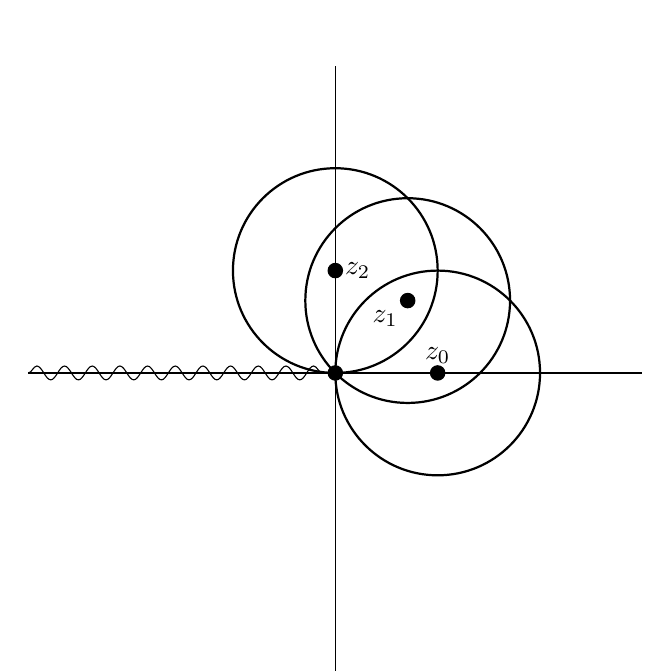
\begin{tikzpicture}[scale=1.3]
    \draw (0,-3) -- (0,3);
    \draw (-3,0) -- (3,0);
    \draw [thick] (1,0) circle (1);
    \draw [thick] (0.707,0.707) circle (1);
    \draw [thick] (0,1) circle (1);
    \filldraw [black] (1,0) circle (2pt) node[anchor=south]{$z_0$};
    \filldraw [black] (0.707,0.707) circle (2pt) node[anchor=north east]{$z_1$};
    \filldraw [black] (0,1) circle (2pt) node[anchor=west]{$z_2$};
    \filldraw [black] (0,0) circle (2pt);
    \path [draw=black,snake it](-3,0) -- (0,0);
  \end{tikzpicture}
  \caption{Analytic continuation of $\ln z$ via Taylor series centered on $z_0$, $z_1$, and $z_2$. The dot in the center is the pole and the wavy line to the left is the branch cut.}
  \label{fig:ln-analytic-continuation}
\end{figure}

Qualitatively speaking, we've shown that the divergence of (\ref{eqn:log-expansion-0}) was a red herring except at $z=0$. The function was perfectly well defined.

Or was it? There is still one property left to check; if we analytically continue in some path that starts at $z=1$, encircles the origin, and comes back to $z=1$, do we reproduce the same value of $\ln 1$? Perhaps surprisingly, the answer to this question is no; originally $\ln 1 = 0$ but the analytically continued version states $\ln 1 = 2\pi$.\footnote{In the case of the logarithm, it is simple to find the $2\pi$ offset which analytical continuation produces. It happens that $\ln(re^{i\theta})$, where $r$ and $\theta$ are real, is $\ln r + i\theta$. Check this by exponentiating $\ln r + i\theta$ and confirming it is equal to $re^{i\theta}$. Then defining $z_i$ along a circle of radius $r=1$ keeps increasing the imaginary component of $z_i$ as $\theta$ is increased until the circle is complete and the analytical continuation has accumulated a $2\pi i$ offset.} It cannot be that $\ln 1 = 0$ and $2\pi$ at the same time.

This problem illustrates the weakness of analytical continuation. It allows a smooth function to be defined anywhere except at a pole, but it may induce inconsistencies like constant offsets in the value of the function. We fix these by defining a ``branch cut,'' which is an arbitrary path that connects to the simple pole and extends to infinity at which we say $\ln z$ is undefined. That way, the circular path used above to create an inconsistency is interrupted by the branch cut and the argument can no longer be made. This branch cut is represented with a wavy line in Figure \ref{fig:ln-analytic-continuation} and chosen to lie along the negative real axis by convention. In general, any pole in a function generated by analytical continuation should have a branch cut attached to it.For example, $\sqrt{z}$ also has a branch cut, conventionally chosen to lie along the negative real axis as well.

Awareness of the poles and branch cuts in a complex function is a crucial trick when it comes to Taylor expanding or integrating a function. The connection between integration and poles is worked out in the next chapter.


\section{Residue Theorem}
\label{sec:ca-residue}
This section is on the integrals of complex functions such as $f(z)$. Like in vector calculus, when we integrate a function $\int_\gamma dz\, f(z)$ we must specify a curve $\gamma$ and we define the integral in the usual way using Riemann sums. The parametrization of the curve is unimportant, but the location of the curve in complex space is. In vector calculus a two-dimensional vector field $\bm f(\bm z)$ obeys Green's theorem for integration around a closed contour $\gamma$:
\begin{e}
  \oint_\gamma \bm d\ell \cdot \bm f(\bm z) = \int_D d^2 \bm z\, \nabla \times \bm f(\bm z)
\end{e}
where $D$ is the interior of $\gamma$. If $\nabla \times \bm f(\bm z)=0$ everywhere, then the line integral is zero. We would say that $\bm f(\bm z)$ is \emphi{conservative}.

Analytical functions are also conservative in that 
\begin{e}
  \oint_\gamma dz\, f(z) = 0
  \label{eqn:complex-conservative}
\end{e}
when the complex function is defined everywhere inside $\gamma$. An equivalent statement is that one can move $\gamma$ in the complex plane and not change the value of the integral, as long as $f$ is defined everywhere that $\gamma$ was moved through. Both these statements are due to the connection between analytical functions and curl-free vector fields mentioned at the beginning of this section. However, the function might not be defined at a few poles $z_j$ within $\gamma$, and at these points we cannot use Green's theorem. Let us focus on these poles specifically now.

Suppose we have a function $f(z)=z^{-n}$, with a pole of multiplicity $n$ at the origin. We can find the value of a closed integral around the origin by integrating in a nearly-closed contour in a circle around the pole and taking a limit as the ends approach each other. Note that the radius of this circle doesn't matter because if we shrink or expand the circle to another radius, we do not pass the curve through any poles, so that the value of the integral doesn't change.

Complex functions obey the fundamental theorem of calculus:
\begin{e}
  \int_a^b dz\, f(z) = F(b)-F(a)\qquad \mathrm{where}\qquad \frac{dF}{dz} = f(z).
\end{e}
A function $F(z)$ is generally called an \emphi{antiderivative} of $f$.
We changed notation here by not specifying $\gamma$ and instead only specifying its endpoints. This is allowed because, as we just learned, $\gamma$ may be moved through space where $f$ is defined so its exact path doesn't matter.

An antiderivative of $z^{-n}$ is $F(z)=z^{1-n}/(1-n)$, just like for real $z$, except when $n=1$ in which case the antiderivative is $F(z)=\ln z$. For $n>1$, $F(z)$ is continuous so that $F(b)-F(a)\rightarrow 0$ as $b\rightarrow a$. It follows that the closed integral around $z^{-n}$ is zero for $n>1$. However, for $n=1$ we have to deal with the branch cut in the logarithm, over which $F(z)$ is \textit{dis}continuous. We've already mentioned that $F(z)$ increases by $2\pi i$ when moving counterclockwise over the branch cut, so that the value of $\int_a^b dz\, z^{-1}$ must likewise be $2\pi i$. To summarize,
\begin{e}
  \oint_a^b dz\, z^{-n} = \begin{cases}0 & n \neq 1 \\ 2\pi i & n = 1\end{cases}.
\end{e}

Returning to integrating an arbitrary function $f(z)$ with poles at $z_j$, by definition $f(z)$ can be expanded around a pole as follows:
\begin{e}
  f(z) = \frac{a_{-m}}{(z-z_j)^m} + \frac{a_{1-m}}{(z-z_j)^{m-1}} + \dots = \sum_{n=-m}^\infty a_n (z-z_j)^n.
\end{e}
The integral of this function is then zero for each term except $n=-1$, where it is $2\pi i a_{-1}$. We generally write the coefficient $a_{-1}$  of this Taylor series centered at $z_j$ as $a_{-1} = \Res f(z_j)$. Thus
\begin{e}
  \oint_\gamma dz f(z) = 2\pi i \sum_{z_j} \Res f(z_j)
  \label{eqn:residue-theorem}
\end{e}
where $z_j$ are the poles inside $\gamma$.

(\ref{eqn:residue-theorem}) is an incredibly powerful theorem. It can be used to integrate even very complicated functions over closed contours. It can even be used to perform integrals over non-closed contours, by extending the contour through some region of space where we know $f(z)$ is small until the contour becomes closed. For example, we can easily find that 
\begin{e}
  \int_{-\infty}^\infty \frac{dx}{1+x^2} = \pi
\end{e}
via the Residue theorem. First we split the integrand into partial fractions to find the residue:
\begin{e}
  \frac{1}{2}\int_{-\infty}^\infty dx \parens{\frac{i}{x+i} - \frac{i}{x-i}}.
\end{e}
The function has poles at $z=\pm i$, with $\Res f(i) = -i$ and $\Res f(-i)=i$. To make a closed curve, we can close the contour in an enormous loop with very large $|z|$ from the $+\infty$ of the real axis to the $-\infty$ side. This can be done over the real line, in which case the curve will run counterclockwise and enclose the $+i$ pole, or it can be done under the real axis in which case it will run clockwise and enclose the $-i$ pole. Both these answers should be consistent, and they are. The two poles have opposite residues, but integrating over a clockwise curve flips the sign of the integral so that the result for both is
\begin{e}
  \int_{-\infty}^\infty \frac{dx}{1+x^2} = 2\pi i \parens{\frac{1}{2}(-i)} = \pi.
\end{e}

\section{The Gamma Function}
\label{sec:ca-gamma}

We conclude our function on special analysis with the Gamma function, $\Gamma(z)$. $\Gamma(z)$ is one of many special functions, much like the Riemann zeta function $\zeta(z)$, which are discussed in conjunction with complex analysis because their properties are so much easier to understand in the context of complex variables. Nevertheless, when $\Gamma(z)$ appears in physics, a real argument is usually used.

The Gamma function is a crucial function that appears in QFT due to its relation to the surface area of a sphere, discussed in the next chapter. It is also relevant to statistics and can be helpful in computing miscellaneous integrals as well. It is a generalization of the factorial:
\begin{e}
  \Gamma(n+1) = n!
\end{e}
for integer $n$. A consistent definition that works for all $\Re z > 0$ is 
\begin{e}
  \Gamma(z) = \int_0^\infty dt\, t^{1-z} e^{-t}.
  \label{eqn:gamma}
\end{e}
One can check that this definition is consistent with the factorial by showing that 
\begin{e}
  \Gamma(x+1)=x\Gamma(x)
  \label{eqn:gamma-recursion}
\end{e}
and $\Gamma(0)$, which are also properties of factorials. The proof of this fact and other properties of the Gamma function are left to other books.

(\ref{eqn:gamma}) defines a Gamma function is analytic and smoothly connects all the values of the factorial on the positive real axis. Using analytical continuation, we can extend the function to the negative real axis, where it has poles at every negative integer and at zero (Figure \ref{fig:gamma}). At the zero pole, $\Gamma(z)$ has a convenient expansion:
\begin{e}
  \Gamma(\epsilon) = \frac{1}{\epsilon} - \gamma_E + \mathcal{O}(\epsilon)
\end{e}
which generalizes to 
\begin{e}
  \Gamma(-n + \epsilon) = \frac{(-1)^n}{n!}\parens{\frac{1}{\epsilon} - \gamma_E + \sum_{j=1}^n\frac{1}{j}} + \mathcal{O}(\epsilon)
\end{e}
where $\gamma_E \approx 0.57721$ is the Euler-Mascheroni constant.

\begin{figure}
  \centering
  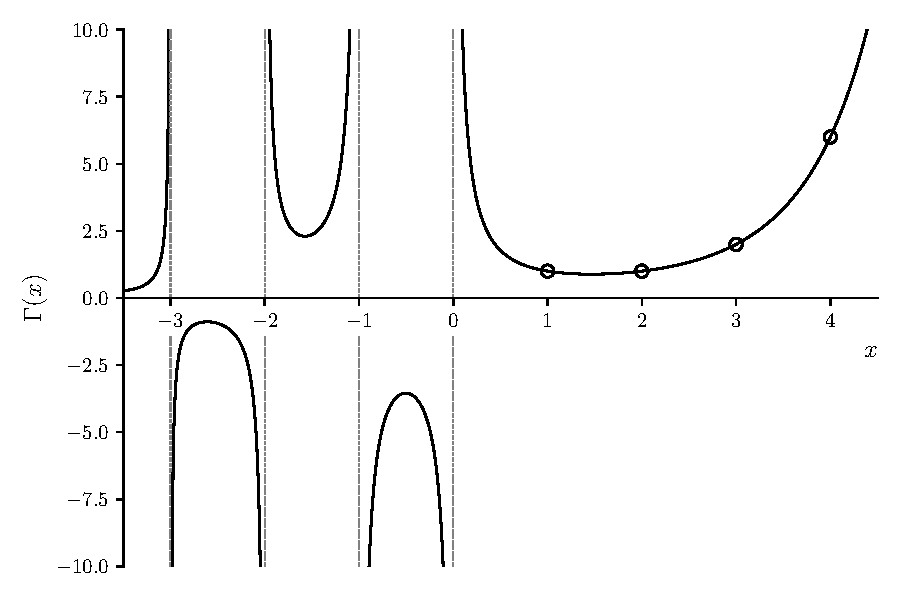
\includegraphics[width=\linewidth]{figs/gamma.pdf}
  \caption{The Gamma function, $\Gamma(x)$ on the real line. Open circles represent the value of $(x+1)!$, and dotted vertical lines are the poles at every non-positive integer.}
  \label{fig:gamma}
\end{figure}

Another useful formula is the values of the Gamma function at half-integers:
\begin{e}
  \Gamma\parens{z+\frac{1}{2}} = \frac{\sqrt{\pi}}{4^{z-\frac{1}{2}}}\frac{\Gamma(2z)}{\Gamma(z)}
\end{e}
which reduces to the special case of $\Gamma(\frac{1}{2}) = \sqrt{\pi}$. The Gamma function can also be used to aid in evaluating the following integral 
\begin{e}
  B(a,b) = \int_0^1 dt\, t^{a-1} (1-t)^{b-1}
  \label{eqn:beta-function}
\end{e}
which is called the \emphi{Beta function}. It appears in QFT as well as in probability and various trigonometric functions. It is related to the Gamma function via
\begin{e}
  B(a,b) = \frac{\Gamma(a)\Gamma(b)}{\Gamma(a+b)}.
  \label{eqn:beta-to-gamma}
\end{e}
Below, we use the Beta and Gamma functions to compute the surface area of a $d$-dimensional sphere.

\subsection{Surface Area of Spheres}
In physics, integrals over quantities which are rotationally symmetrical are very common. Such integrals can be separated into a radial part and an angular part, even in an arbitrary $d$-dimensional space, by integrating over $d$-dimensional spheres like so
\begin{e}
  \int d^d x\, f(|x|) = \parens{\int dr\, r^{d-1} f(r)}A_d
  \label{eqn:radial-integral}
\end{e}
where $A_d$ is the surface area of the $d$-dimensional unit sphere. For example, for $d=3$, we have $A_d = 4\pi$ and in $d=2$ we have $A_d=2\pi$.

The task of this section is to find the surface area of this $d$-dimensional sphere as a function of $d$, which we will do via recursion. Suppose we know the area $A_{d-1}$. This knowledge allows us to ignore all the $d-1$ axes of this sphere and project them down into a single axis $\hat x$, with the $d$th axis $\hat y$ being perpendicular to $\hat x$. Now we can think two-dimensionally.

\begin{figure}
  \centering
  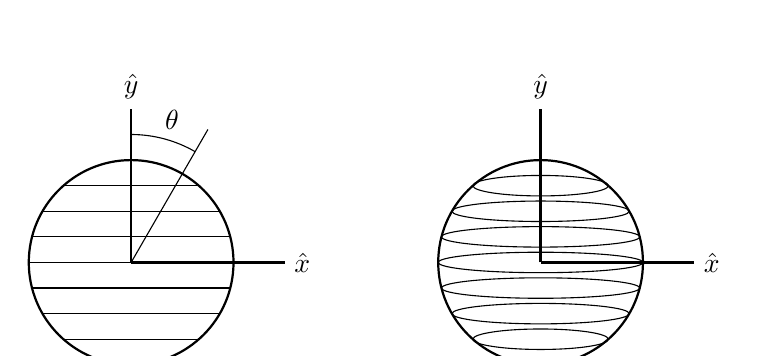
\begin{tikzpicture}[scale=1.3]
    \draw [thick] (-2,0) circle (1);
    \draw [thick] (-2,0) -- (-2,1.5);
    \draw [thick] (-2,0) -- (-0.5,0);
    \draw (-2,0) -- (-1.25,1.29903810567665);
    \draw (-2,1.25) arc (90:60:1.25);
    \draw (-1.6,1.2) node[anchor=south] {$\theta$};
    \draw (-2,1.5) node[anchor=south] {$\hat y$};
    \draw (-0.5,0) node[anchor=west] {$\hat x$};
    \draw (-3,0) -- (-1,0);
    \draw (-2.968245836551854,0.25) -- (-1.0317541634481457,0.25);
    \draw (-2.8660254037844384,0.5) -- (-1.1339745962155614,0.5);
    \draw (-2.6614378277661475,0.75) -- (-1.3385621722338523,0.75);
    \draw (-2.968245836551854,-0.25) -- (-1.0317541634481457,-0.25);
    \draw (-2.8660254037844384,-0.5) -- (-1.1339745962155614,-0.5);
    \draw (-2.6614378277661475,-0.75) -- (-1.3385621722338523,-0.75);


    \draw [thick] (2,0) circle (1);
    \draw [thick] (2,0) -- (2,1.5);
    \draw [thick] (2,0) -- (3.5,0);
    \draw (2,1.5) node[anchor=south] {$\hat y$};
    \draw (3.5,0) node[anchor=west] {$\hat x$};
    \draw (2, 0) ellipse (1 and 0.1);
    \draw (2, 0.25) ellipse (0.9682458365518543 and 0.1);
    \draw (2, 0.5) ellipse (0.8660254037844384 and 0.1);
    \draw (2, 0.75) ellipse (0.6614378277661475 and 0.1);
    \draw (2, -0.25) ellipse (0.9682458365518543 and 0.1);
    \draw (2, -0.5) ellipse (0.8660254037844384 and 0.1);
    \draw (2, -0.75) ellipse (0.6614378277661475 and 0.1);
  \end{tikzpicture}
  \caption{Stacking $d-1$-dimensional spheres to form a $d$-dimensional sphere for $d=2$ (\textit{left}) and $d=3$ (\textit{right}).}
  \label{fig:sphere-surface-area}
\end{figure}

The $d$-dimensional unit sphere corresponds to a unit circle on the $\hat x$ and $\hat y$ axes, which we parameterize by the angle $\theta$ between some point on the circle and the positive $\hat y$ axis. The $d$-dimensional unit sphere is created by stacking many $d-1$-dimensional spheres horizontally on top of each other like vertical lines inside the circle, meaning that the radius of one of these $d-1$-spheres is $r=\sin\theta$. It contributes an area of $dA = A_{d-1}\sin^{d-2}\theta d\theta$ to the total area. The $\sin^{d-2}\theta$ is present because surface area of the $d-1$ dimensional non-unit sphere is $A_{d-1}$ (the unit sphere area) times the radius to the $d-2$th power. This integration scheme is shown in Figure \ref{fig:sphere-surface-area}. Thus, the $d$-sphere surface area is 
\begin{es}
  A_d &= A_{d-1}\int_0^\pi d\theta\,\sin^{d-2}\theta \\
  &= -A_{d-1}\int_0^\pi d(\cos\theta)\,\sin^{d-3}\theta\\
  &= A_{d-1}\int_{-1}^1 dx\,\parens{1-x^2}^{\frac{d-3}{2}}\\
  &= A_{d-1}\int_0^1 dt\,t^{-\frac{1}{2}}\parens{1-t}^{\frac{d-3}{2}}
\end{es}
where in the second line we substituted variables from $\theta \rightarrow \cos\theta$, in the third line we expressed $\sin\theta = \sqrt{1-\cos^2\theta}$, and in the last line we substituted variables $x^2 \rightarrow t$. The reader may recognize the last integral as a Beta function $B(\frac{1}{2}, \frac{d-1}{2})$, so we may immediately write it in terms of $\Gamma$ functions:
\begin{e}
  A_d = A_{d-1} \frac{\Gamma\parens{\frac{1}{2}}\Gamma\parens{\frac{d-1}{2}}}{\Gamma\parens{\frac{d}{2}}} = A_{d-1} \sqrt{\pi}\frac{\Gamma\parens{\frac{d-1}{2}}}{\Gamma\parens{\frac{d}{2}}}.
\end{e}
Now we must turn the above recursive equation into a formula for $A_d$, but fortunately this is not difficult due to the $\Gamma$ function's own recursion relation (\ref{eqn:gamma-recursion}). The following formula checks out:
\begin{e}
  A_d = \frac{2\pi^{d/2}}{\Gamma\parens{\frac{d}{2}}}.
  \label{eqn:surface-area-sphere}
\end{e}

(\ref{eqn:surface-area-sphere}) draws a fascinating and unexpected connection between the Gamma function, which descended from factorials, and spheres. Without extending the factorials to the half-integers via the Gamma function, we could not have written (\ref{eqn:surface-area-sphere}) down.
\chapter{Review of Group Theory and Lie-Groups}

\section{What are Groups?}

\section{Generators of Groups}

\section{Angular Momentum and the Lie Bracket}

\section{Important Groups}


% \part{Excluded stuff}

% \chapter{\texorpdfstring{$\phi^4$}{Phi-four} Theory}

\section{Feynman rules for \texorpdfstring{$\phi^4$}{Phi-four} Theory}

% \section{$\phi\phi\rightarrow \phi\phi$ Interaction}

% \section{Higher Order Terms}

% \section{$\phi^3$ Theory Decay?}
% \chapter{Sombrero Theory}

\section{Spontaneous Symmetry Breaking}

\section{Massless decay?}

I would do this (1) if the sombrero model actually has $\theta\rightarrow \theta\theta$ decay, and (2) if this section weren't already too huge (because I could also put it in $\phi^3$)\footnote{https://arxiv.org/pdf/hep-th/9508018.pdf}.
% \chapter{Lagrangians and the Principle of Least Action}

\section{The Euler Lagrange equation}

\section{Example: Harmonic Oscillator}

\section{Example: Electromagnetic Action}
% Stern Gerlach experiment in rel qft?

\backmatter
\appendix

\chapter{Properties of the $\gamma^\mu$ matrices}
\label{app:gamma}
\chapter{Grassmann numbers}
\label{app:grassmann}
Above, we stated the fact that spinor operators anticommute. But in the QFT principle of least action, only the left hand side (the $n$PTFs) contain spinors. The right hand side is a path integral over the complex values of the field, which in this case is just a vector of four numbers $\phi_i$ to emulate the four operators in the $\hat \phi$ spinor.

However, the anti-commuting nature of the fermion must be taken into account. To do so, we define a new number line of anticommuting numbers, which are called Grassmann numbers. These will represent the possible fermionic field values in the path integral of the QFT principle of least action.

The definition of these numbers is that, for any two Grassmann numbers $\eta$ and $\theta$,
\begin{equation}
  \theta \eta = -\eta \theta.
\end{equation}
A special case is that $\theta^2 = \eta^2 = 0$. These numbers may seem like odd, but future investigation will show that their properties are very simple do to their square vanishing in this way. For example, the Taylor series of any function $f(\theta)$ is $\alpha + \beta\theta + \gamma\theta^2 + \dots$ for more Grassmann numbers constants $\alpha,\beta,\gamma$, etc. But since $\theta^2 = 0$, this is just 
\begin{e}
  f(\theta) = \alpha +  \beta\theta.
\end{e}
All functions are therefore linear.

Integration is likewise simple for Grassmann numbers. We will only need integrals over the entire space of Grassmann numbers --- the equivalent of integrals from $-\infty$ to $\infty$ on the real line --- and therefore the integral of a function $\alpha + \beta \theta$ should depend only on $\alpha$ and $\beta$. Furthermore, substitution of variables implies that $\int d\theta\, f(\theta) = \int d\theta\, f(\theta + \eta)$, so that
\begin{e}
  \int d\theta\, \alpha +  \beta\theta = \int d\theta\, \alpha +  \beta(\theta + \eta) = \int d\theta\, (\alpha + \beta \eta) + \beta \theta.
\end{e}
The intercept $\alpha$ of the function has been shifted by this substitution of variables, so the integrand can only be proportional to $\beta$. By convention, we set the integrand equal to $\beta$.
\begin{e}
  \int d\theta\, \alpha +  \beta\theta = \beta.
\end{e}
For multidimensional integrals, we treat the volume element $d\theta$ as another Grassmann number, so that $d\theta\,d\eta = -d\eta \, d\theta$. By convention, we set
\begin{e}
  \int d\eta\, d\theta\, \theta \eta = 1 \implies \int d\theta\, d\eta\, \theta \eta = -1.
\end{e}

The last detail we need is that of complex Grassmann numbers, which are defined just like normal complex numbers: $\psi = \theta + i\eta$. Their complex conjugate is $\psi^* = \theta - i\eta$.

\subsection{Wick's theorem for Grassmann numbers}
\jtd{Do this}


\chapter{Particles of the Standard Model}
\chapter{Encyclopedia of Quantum Field Theories}
\chapter{Important Formulas}
\chapter{Second Quantization}
\chapter{Lattice QCD}
\chapter{Spin 2 Particles and Gravitons}
\chapter{Noether's Theorem}
\label{app:noether}

{
\small
\printindex
}
\end{document}